% E-scooter pothole impacts and front-wheel size (Oxford): preprint.
% Build:  latexmk -lualatex main.tex      (from the paper/ folder)
% Sections live in sections/*.tex; figures in figures/; bibliography = ../references.bib
% (the project's master bibliography, checked entries only; see ../REFERENCES.md).
\documentclass[11pt,a4paper]{article}

% ---- Fonts and language (LuaLaTeX: Unicode symbols such as >= and rho typeset directly)
\usepackage{fontspec}
\usepackage{unicode-math}
\setmainfont{Libertinus Serif}
\setsansfont{Libertinus Sans}
\setmathfont{Libertinus Math}
\usepackage[british]{babel}

% ---- Page layout
\usepackage[margin=25mm]{geometry}
\usepackage{setspace}
\setstretch{1.12}
\usepackage{microtype}
\usepackage{parskip}

% ---- Tables, figures, lists
\usepackage{booktabs}
\usepackage{longtable}
\usepackage{array}
\usepackage{calc}
\usepackage{graphicx}
\graphicspath{{figures/}}
\usepackage{float}
\usepackage{pdflscape}          % landscape pages (spot table, Appendix C)
\usepackage{colortbl}           % light grey table rules (\arrayrulecolor)
\usepackage{needspace}          % keep table-group headings with their rows
\usepackage{qrcode}             % QR codes in the spot table, for printed copies
\usepackage[section]{placeins}   % figures/tables stay within their section
\usepackage[font=small,labelfont=bf,margin=0pt]{caption}
\usepackage{enumitem}
\setlist{itemsep=2pt,topsep=4pt}
% Pandoc-generated tables and lists use these helpers.
\providecommand{\tightlist}{\setlength{\itemsep}{0pt}\setlength{\parskip}{0pt}}
\newcounter{none}   % Pandoc marks uncaptioned longtables with \LTcaptype{none}
\makeatletter
\def\fps@figure{htbp}
\makeatother

% ---- Bibliography: author-year, Biber
\usepackage[style=authoryear,backend=biber,maxcitenames=2,maxbibnames=8,
            uniquelist=false,giveninits=true,urldate=long,dashed=false]{biblatex}
\addbibresource{../references.bib}
% Undated web sources: show "n.d." rather than the access (urldate) year as their date.
\DeclareLabeldate{\field{date}\field{year}\field{eventdate}\field{origdate}\literal{nodate}}

% ---- Links (last)
\usepackage{xcolor}
\definecolor{linkblue}{HTML}{1C5CAB}
\definecolor{rulegray}{HTML}{E3E2DE}
\usepackage[colorlinks=true,linkcolor=linkblue,citecolor=linkblue,urlcolor=linkblue]{hyperref}
\usepackage{xurl}

% ---- Appendix numbering: Figure A1, Table B2, ... (counters restart in each appendix)
\newcommand{\appendixnumbering}{%
  \counterwithin*{figure}{section}\counterwithin*{table}{section}%
  \renewcommand{\thefigure}{\Alph{section}\arabic{figure}}%
  \renewcommand{\thetable}{\Alph{section}\arabic{table}}}

\title{Pothole impacts on rental e-scooters and the case for a larger front wheel:\\
       measurements in Oxford and a dynamics model}
\author{[Author name]\thanks{[MSc programme, university]. Contact: [email].}}
\date{Draft, \today}

\begin{document}
\maketitle

\begin{abstract}
\noindent [Abstract: to be written once all sections are final.]
\end{abstract}

% Introduction. Argument agreed 2026-10-07 (DOCUMENTATION.md 12); sources checked in
% REFERENCES.md ("Literature search ...", 2026-10-08). Each citation is used only for what
% the "use for" column there allows.
% Wheel sizes: Voiager 5 = 11/10 in from the author's tyre photographs (2026-10-09,
% tyre-images/, scripts/tyre_figure.py); the reported 10 in is kept only as a reference.
\section{Introduction}\label{sec:intro}

\subsection{Background}

Rental e-scooters are ridden on British roads under trials authorised by the Department
for Transport (DfT). They are the only e-scooters that may legally be used on
public roads; privately owned e-scooters may be ridden only on private land with the
landowner's permission \autocite{dft2026users}. The design of every legal e-scooter on a
British road is therefore set by a small number of rental operators, within the vehicle
rules of the national trials and of the local areas that host them.

In 2025, 10 e-scooter riders were killed and about 410 seriously injured in reported road
collisions in Great Britain, and 384 of the 1,377 reported collisions involving an
e-scooter (28\%) involved no other vehicle \autocite{dft2026factsheet}. A recent systematic review found falls to be the most common
type of e-scooter accident, with human, vehicle and environmental factors all contributing
\autocite{nathania2026}. Riders themselves name infrastructure hazards among the risks they
perceive \autocite{anke2025}, and in a study of injured riders in Washington, DC, injuries
sustained on the road were about twice as likely to be of moderate or greater severity as
those sustained elsewhere \autocite{cicchino2021}.

Small wheels are a plausible part of the vehicle side of this problem. A wheel that drops into
a pothole meets the far edge at a steeper angle the smaller it is, and the front wheel of a
scooter both steers and takes the first impact. Using a multibody model of an e-scooter with
10~in wheels, \textcite{posirisuk2022} found that 3~cm deep potholes caused no falls, while
6~cm deep potholes caused falls in 41 of 60 simulated cases, with the rider pitching forward
over the handlebar. Other models have examined falls caused by striking a kerb
\autocite{fournier2023}, and experimental tests of small-wheeled personal vehicles found
compact, small-wheeled devices less stable than those with larger wheels; their authors
recommend wheels of at least 14~in and front suspension \autocite{paudel2025}. Instrumented
tests have related e-scooter stability and comfort to vehicle specifications
\autocite{leoni2022}, and vibration and comfort on e-scooters have been measured and modelled
\autocite{canomoreno2022,ventura2024,vacamichilena2026}. Smartphones and other low-cost
sensors have also been used to map potholes and road roughness from moving vehicles
\autocite{eriksson2008,zang2018}.

\subsection{The regulatory gap}

Neither the national trial guidance \autocite{dft2024guidance} nor the legal definition of a
trial e-scooter \autocite{si2020_663} sets a minimum wheel size. The guidance's stability
tests include riding through a depression 1~m long and 5~cm deep with vertical walls.
London's trial goes further: since November 2022, its rental e-scooters must have a front
wheel of at least 11~in and a rear wheel of at least 9~in \autocite{tfl2022tender}, and
Transport for London describes its vehicle standards, including larger wheels, as going
beyond the national ones \autocite{tfl2023press}. Outside London the
national rules set no wheel size; London's 11~in is the only minimum we found, although we
did not check the contracts of individual trial areas, which could add their own.

The Voi Voiager 5, the model ridden in this study in Oxford \autocite{voi2026support_rec01,
voi2026support_rec0203,occ_trial}, sits at that minimum. Published sources give its wheels
as 10~in without separating front and rear \autocite{levy_voiager5,alsalkini2023}, but the
author's photographs of a parked Voiager 5 in Oxford show a 60/55-8.5 front tyre and a
60/55-7.5 rear tyre (Figure~\ref{fig:tyres}). Their nominal outer diameters are 282~mm
(11.1~in) and 257~mm (10.1~in): the front wheel is larger than the rear and meets London's
11~in minimum by about 2.5~mm. We use these photographed sizes, written 11/10, throughout.
The model was introduced in 2022 with a larger front wheel, deeper tyre tread and greater
shock absorption than its predecessor \autocite{roadcc2022voiager5}, and was still being
deployed in new trial areas in 2025 \autocite{essex2025voi}. The open question is
whether a front wheel at London's minimum is enough, and what a larger one would change.

\begin{figure}[htbp]
\centering
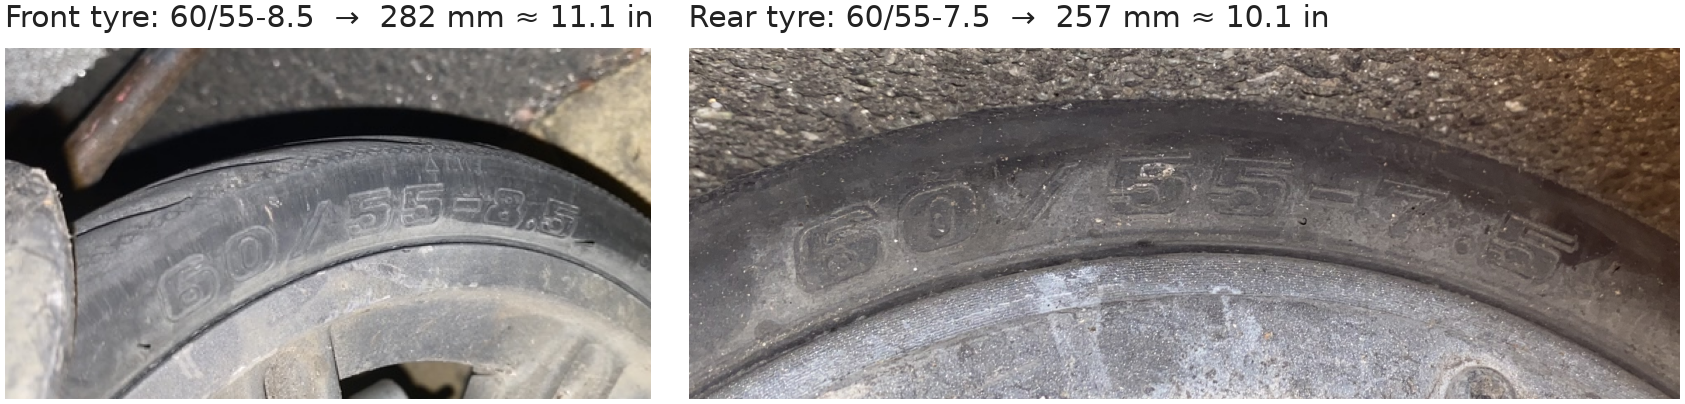
\includegraphics[width=\linewidth]{fig_tyres.png}
\caption{Tyre sidewall size codes of a Voi Voiager 5 parked in Oxford, photographed by the
author on 9 October 2026 (crops). Metric code width/aspect ratio-rim diameter; nominal
outer diameter = rim + 2 $\times$ width $\times$ aspect ratio. The photographed scooter is the
same model as the three ridden scooters (Voiager 5).}\label{fig:tyres}
% The author verified that the photographed scooter is a Voiager 5 (2026-10-10).
\end{figure}

\subsection{Research question and contributions}

This paper asks whether pothole impacts on the Voiager 5 reach levels associated with loss of
stability, and whether a front wheel larger than its current 11~in would reduce them. It
tests a specific
hypothesis that could turn out to be false:

\begin{quote}
Because the front wheel both steers and takes the peak load at impact, enlarging the front
wheel alone gives most of the stability benefit of enlarging both wheels.
\end{quote}

If the hypothesis held, a front-wheel minimum such as London's would capture most of the
benefit of larger wheels, at lower cost than enlarging both. If it failed, for example
because the rear wheel's impact also caused falls, a front-only rule would be insufficient.

The work has two parts. \textbf{Part A} (Section~\ref{measuring-what-riders-experience-on-the-road})
measures what a rider experiences: three legal rides on Voiager 5 scooters in Oxford, recorded
with a handlebar-mounted smartphone, give the number, size and location of sudden vertical
impacts, which are compared with public pothole reports. The recording method itself is checked,
including whether it can tell riding from walking. \textbf{Part B}
(Sections~\ref{methods-modelling-the-effect-of-wheel-size}
and~\ref{results-what-a-larger-front-wheel-would-change}) uses a geometry model and a planar
dynamics model of scooter and rider to compare the current 11/10 wheels with a smaller
10/10 reference, with larger front wheels alone and with larger wheels front and rear. The measured impacts provide a consistency check
for the model, not a validation.

Compared with earlier work, the contributions are: measurement of discrete impacts on a rental
e-scooter in ordinary use, rather than comfort vibration; repeated impacts at the same places
across rides, compared with what the public had reported; and a direct test of whether a
larger front wheel alone performs like larger wheels front and rear. Section~\ref{sec:discussion}
discusses what the results do and do not show and what they suggest for trial rules.

% Converted from part_a_measured_impacts.md by scripts/md_to_latex.py; edit this file.
% DRAFT v0.1 (2026-10-08). Part A of the paper: measured impacts on the road (three rides).
% Citations use Pandoc keys from ../references.bib, e.g. [@sensorlogger].
% Every number is taken from outputs/ or paper/figures/part_a_numbers.json (made by
% scripts/paper_part_a.py); sources are noted in HTML comments. Re-check them if any
% script is rerun. Individual recordings are reported in appendix_recordings.md.
% Decisions (2026-10-08): Part A uses all three recordings; combined results in the main
% text, per-recording results in the appendix; road bumps are not part of the paper.
% Table numbering: Part A uses Tables 1-3; Part B continues from Table~\ref{tab:4}.

\section{Measuring what riders experience on the road}\label{measuring-what-riders-experience-on-the-road}

\subsection{Data}\label{data}

\textbf{Rides.} One rider recorded three rides on Voi rental e-scooters in Oxford, ridden
legally within the national e-scooter trial \autocite{dft2024guidance,occ_trial}: one on
3 October 2026 (vehicle SZ22) and two on 7 October 2026 (vehicles UPAR and BTLZ). Voi
customer support confirmed that all three vehicles were Voiager 5 scooters
\autocite{voi2026support_rec01,voi2026support_rec0203}. The rides covered parts of Marston
Road, Morrell Avenue, Old Road (Headington), Headington Road and connecting streets.
Only the rider's own rides were recorded.

\textbf{Recording.} An iPhone 11 Pro Max was mounted on the handlebar and recorded with the
Sensor Logger app, version 1.67.1 \autocite{sensorlogger}. The app logged user acceleration
(gravity removed) and the gravity vector from the iOS sensor fusion
\autocite{apple_cmdevicemotion}, the raw accelerometer, the gyroscope (all at 100 Hz) and GPS
(about 1 Hz). The phone was set up before each ride and not touched while riding.

% outputs/recordings/<rec>/impact_stats.json; data/README.md

\begin{longtable}[]{@{}
  >{\raggedright\arraybackslash}p{(\linewidth - 10\tabcolsep) * \real{0.1667}}
  >{\raggedright\arraybackslash}p{(\linewidth - 10\tabcolsep) * \real{0.1667}}
  >{\raggedright\arraybackslash}p{(\linewidth - 10\tabcolsep) * \real{0.1667}}
  >{\raggedright\arraybackslash}p{(\linewidth - 10\tabcolsep) * \real{0.1667}}
  >{\raggedright\arraybackslash}p{(\linewidth - 10\tabcolsep) * \real{0.1667}}
  >{\raggedright\arraybackslash}p{(\linewidth - 10\tabcolsep) * \real{0.1667}}@{}}
\caption{The three rides. Riding time and distance count only travel at 7 km/h or faster (section 2.3).}\label{tab:1}\tabularnewline
\toprule\noalign{}
\begin{minipage}[b]{\linewidth}\raggedright
Ride
\end{minipage} & \begin{minipage}[b]{\linewidth}\raggedright
Date, start (local)
\end{minipage} & \begin{minipage}[b]{\linewidth}\raggedright
Vehicle (Voiager 5)
\end{minipage} & \begin{minipage}[b]{\linewidth}\raggedright
Recorded
\end{minipage} & \begin{minipage}[b]{\linewidth}\raggedright
Riding
\end{minipage} & \begin{minipage}[b]{\linewidth}\raggedright
Distance ridden
\end{minipage} \\
\midrule\noalign{}
\endfirsthead
\toprule\noalign{}
\begin{minipage}[b]{\linewidth}\raggedright
Ride
\end{minipage} & \begin{minipage}[b]{\linewidth}\raggedright
Date, start (local)
\end{minipage} & \begin{minipage}[b]{\linewidth}\raggedright
Vehicle (Voiager 5)
\end{minipage} & \begin{minipage}[b]{\linewidth}\raggedright
Recorded
\end{minipage} & \begin{minipage}[b]{\linewidth}\raggedright
Riding
\end{minipage} & \begin{minipage}[b]{\linewidth}\raggedright
Distance ridden
\end{minipage} \\
\midrule\noalign{}
\endhead
\bottomrule\noalign{}
\endlastfoot
1 & 3 Oct 2026, 18:30 & SZ22 & 13.7 min & 9.6 min & 2.89 km \\
2 & 7 Oct 2026, 10:37 & UPAR & 35.3 min & 5.9 min & 1.48 km \\
3 & 7 Oct 2026, 13:38 & BTLZ & 11.4 min & 6.3 min & 1.71 km \\
All & & & 60.4 min & 21.8 min & 6.08 km \\
\end{longtable}

Ride 2 also includes a walk after the rental ended and a long period with the phone at
rest; these parts are excluded from the impact analysis by the speed rule and were used
to check the recording method (section 2.2).

\subsection{Checking the recording method}\label{checking-the-recording-method}

Before using the phone data, we checked that they are internally sound and that riding
can be told apart from walking. The full method and results are given in Appendix B;
the main points are summarised here.

\textbf{Data quality.} In all three recordings the motion sensors ran at 99.72 Hz with
sampling intervals of 10.03 ms and no gaps, duplicated or out-of-order timestamps. During
the one period when the phone lay still (ride 2, after the walk), the acceleration noise
was about 0.001 g and the raw acceleration magnitude was 0.994 g, both small against the
1.0 g impact threshold used below. The phone's own estimate of GPS horizontal accuracy
had a median of 11--14 m per ride. These checks show internal consistency and
plausibility, not absolute accuracy, which would need a reference instrument.

% outputs/sensor_validity/quality_summary.csv

\textbf{Riding versus walking.} Walking and riding were distinguished with simple, fixed
rules on 4 s windows. The rules used established features: the vertical acceleration
obtained by projecting onto the gravity direction \autocite{mizell2003}; the share of its power
in the walking step band of 1.2--2.8 Hz, estimated with Welch's method \autocite{welch1967},
around measured mean step frequencies of 1.8--2.0 Hz \autocite{pachi2005}; the autocorrelation at
one step period, a measure of step regularity \autocite{moenilssen2004}; and GPS speed. Similar
signals are used for activity and transport-mode detection with phones
\autocite{kwapisz2011,reddy2010}; our aim was not a new classifier but a check that this app
and phone, mounted on a rental scooter, separate the two.

% outputs/sensor_validity/ground_truth_comparison.csv, walking_onsets.csv

In ride 2 the method found sustained walking from 10:46:47, the first step of a 275 s
walk at 2.04 steps per second (Figure~\ref{fig:1}). This agrees with two references, both with
one-minute precision: the Voi app recorded the rental ending at 10:46, and the rider
recalled walking ``after 10 minutes'' of the recording (10:47). In rides 1 and 3, which
the rider confirmed contained no walking, no walking bout was detected; isolated
walking labels covered 6 s and 8 s, all after the ride had ended. In 1,126 windows where
GPS alone showed riding speed (12 km/h or more), none met the walking criteria. With one
walking episode this shows that the data separate riding from walking; it does not give
a detection rate.

\begin{figure}
\centering
{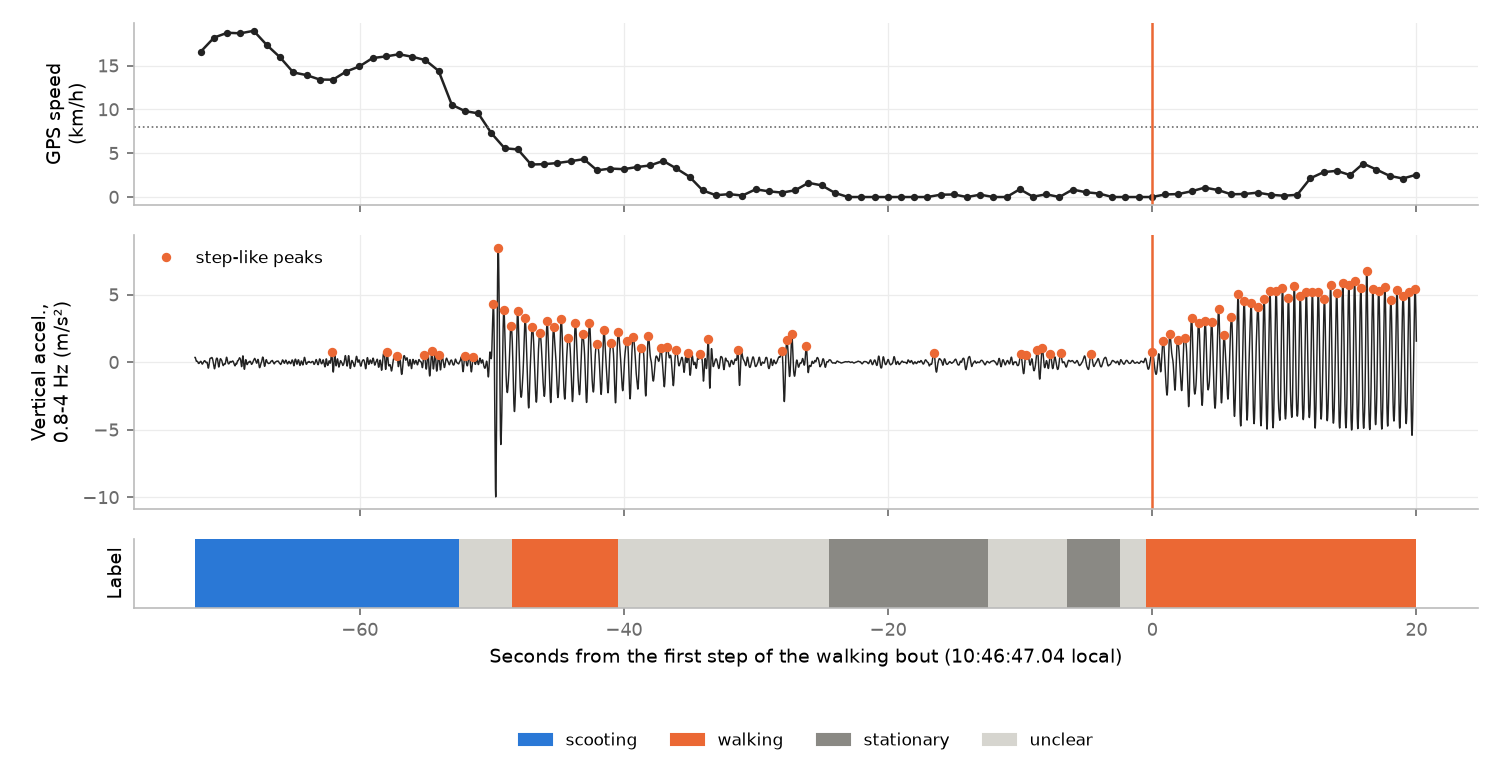
\includegraphics[width=\linewidth]{fig_a1_walk_onset.png}}
\caption{Transition from riding to walking in ride 2. Top: GPS speed; middle: vertical
acceleration (0.8--4 Hz) with step-like peaks; bottom: labels from the window rules. Time
0 is the first step of sustained walking (10:46:47). GPS speed rose only about 12 s after
walking began.}\label{fig:1}
\end{figure}

\textbf{Implications for impact detection.} Two findings bear on the method in section 2.3.
First, walking alone produced 11 peaks of 1.0 g or more (maximum 1.19 g) in ride 2's
walk; the speed rule excluded all of them, and all impacts in ride 2 occurred during
the ride. Second, the GPS-reported speed under-read walking: 3.0 km/h against at least
4.6 km/h from the GPS positions themselves. It was also below the position-based lower
bound in 4 of 6 riding segments, by 0.2--3.2 km/h. Because the speed rule uses the
reported speed, some impacts at low riding speeds may have been excluded; this was not
quantified. Dedicated GPS receivers have also been found to underestimate speed on
curved paths \autocite{witte2004}.

\subsection{Impact detection}\label{impact-detection}

% scripts/impact_map.py; outputs/recordings/<rec>/impacts_params.json

The user acceleration was projected sample by sample onto the upward direction given by
the gravity vector, so that the result does not depend on how the phone sat in its
mount \autocite{mizell2003}. An \textbf{impact} is a peak in the absolute vertical acceleration of at
least \textbf{1.0 g}, at least 0.5 s after the previous one (SciPy \texttt{find\_peaks}
\autocite{virtanen2020scipy}), while the GPS-reported speed was at least \textbf{7 km/h}. The speed
rule excludes getting on and off, stops, walking and handling the phone. Each impact
was located by interpolating the GPS track, using only fixes with a reported accuracy
of 20 m or better. For each impact, the rotation rate of the handlebar (gyroscope) in
the 1.5 s after the impact was divided by that in the 2 s before it; a ratio of 1.5 or
more is reported as \textbf{marked wobble}.

The 1.0 g threshold, the 7 km/h speed rule and the 1.5 wobble ratio are analyst
choices, not established criteria. A fixed threshold in g was used, rather than one set
per ride, so that rides and vehicles can be compared directly.

\subsection{Roads and repeated spots}\label{roads-and-repeated-spots}

% scripts/impact_report.py, scripts/combined_outputs.py, scripts/spot_links.py

Each impact and each second of riding was assigned to a study road if it lay within 20 m
of the road's centreline in OpenStreetMap \autocite{osm,overpass}, and to ``other roads''
otherwise. Rates per km are given only where at least 0.2 km was ridden on a road (an
analyst choice; shorter distances give meaningless rates).

To find places that produce impacts repeatedly, the impacts of all three rides were
pooled and grouped by single-linkage clustering \autocite{sibson1973} with a 30 m distance,
which is larger than the typical GPS error. Each group is a \textbf{spot}, ranked in three
tiers: impacts from two or more separate rides (tier 1), two or more impacts from one
ride (tier 2), and single impacts (tier 3). The rides share one rider, phone and route,
so repeated hits on a spot are repeated measurements of one place, not independent
confirmations.

\subsection{Comparison with FixMyStreet}\label{comparison-with-fixmystreet}

% scripts/fms_compare.py; data/fixmystreet/reports_<rec>.bbox.json

Public road-surface reports were taken from FixMyStreet \autocite{fixmystreet} for each ride's
own area (potholes, carriageway defects, manholes and drain ironwork; reports in two
catch-all categories were kept only if their title described the road surface). An
impact counts as near a report if a report made in the 365 days before that ride lies
within 25 m. Because reports are dense, each rate is compared with a \textbf{route
baseline}: the share of all points along the ridden route that lie within 25 m of
such a report, which is what chance alone would give. With reports from all years
instead of the last 365 days, 70--87\% of route points lie near a report, which is
why only recent reports are used.

\subsection{Results}\label{results}

\subsubsection{Impacts}\label{impacts}

% paper/figures/part_a_numbers.json: per_ride_and_pooled, pooled

The three rides produced \textbf{100 impacts} over 6.08 km of riding, 16.4 per km, or one
every 61 m (Table~\ref{tab:2}). Their median peak was 1.27 g (interquartile range 1.13--1.73 g);
32 reached 1.5 g, 12 reached 2.0 g, and 95\% were at or below 2.68 g (Figure~\ref{fig:2}). One impact,
in ride 3, reached 6.28 g; all others were 2.97 g or less. Thirty-two impacts were
followed by marked wobble, 12 of them also at 1.5 g or more.

\begin{longtable}[]{@{}
  >{\raggedright\arraybackslash}p{(\linewidth - 14\tabcolsep) * \real{0.1250}}
  >{\raggedright\arraybackslash}p{(\linewidth - 14\tabcolsep) * \real{0.1250}}
  >{\raggedright\arraybackslash}p{(\linewidth - 14\tabcolsep) * \real{0.1250}}
  >{\raggedright\arraybackslash}p{(\linewidth - 14\tabcolsep) * \real{0.1250}}
  >{\raggedright\arraybackslash}p{(\linewidth - 14\tabcolsep) * \real{0.1250}}
  >{\raggedright\arraybackslash}p{(\linewidth - 14\tabcolsep) * \real{0.1250}}
  >{\raggedright\arraybackslash}p{(\linewidth - 14\tabcolsep) * \real{0.1250}}
  >{\raggedright\arraybackslash}p{(\linewidth - 14\tabcolsep) * \real{0.1250}}@{}}
\caption{Impacts per ride and pooled. Pooled values describe the three rides together; the rides are not independent samples.}\label{tab:2}\tabularnewline
\toprule\noalign{}
\begin{minipage}[b]{\linewidth}\raggedright
Ride
\end{minipage} & \begin{minipage}[b]{\linewidth}\raggedright
Impacts
\end{minipage} & \begin{minipage}[b]{\linewidth}\raggedright
Per km
\end{minipage} & \begin{minipage}[b]{\linewidth}\raggedright
Median (g)
\end{minipage} & \begin{minipage}[b]{\linewidth}\raggedright
Max (g)
\end{minipage} & \begin{minipage}[b]{\linewidth}\raggedright
≥ 1.5 g
\end{minipage} & \begin{minipage}[b]{\linewidth}\raggedright
≥ 2.0 g
\end{minipage} & \begin{minipage}[b]{\linewidth}\raggedright
Marked wobble
\end{minipage} \\
\midrule\noalign{}
\endfirsthead
\toprule\noalign{}
\begin{minipage}[b]{\linewidth}\raggedright
Ride
\end{minipage} & \begin{minipage}[b]{\linewidth}\raggedright
Impacts
\end{minipage} & \begin{minipage}[b]{\linewidth}\raggedright
Per km
\end{minipage} & \begin{minipage}[b]{\linewidth}\raggedright
Median (g)
\end{minipage} & \begin{minipage}[b]{\linewidth}\raggedright
Max (g)
\end{minipage} & \begin{minipage}[b]{\linewidth}\raggedright
≥ 1.5 g
\end{minipage} & \begin{minipage}[b]{\linewidth}\raggedright
≥ 2.0 g
\end{minipage} & \begin{minipage}[b]{\linewidth}\raggedright
Marked wobble
\end{minipage} \\
\midrule\noalign{}
\endhead
\bottomrule\noalign{}
\endlastfoot
1 & 40 & 13.8 & 1.19 & 2.80 & 6 & 4 & 13 \\
2 & 39 & 26.4 & 1.34 & 2.87 & 15 & 3 & 11 \\
3 & 21 & 12.3 & 1.67 & 6.28 & 11 & 5 & 8 \\
All & 100 & 16.4 & 1.27 & 6.28 & 32 & 12 & 32 \\
\end{longtable}

\begin{figure}
\centering
{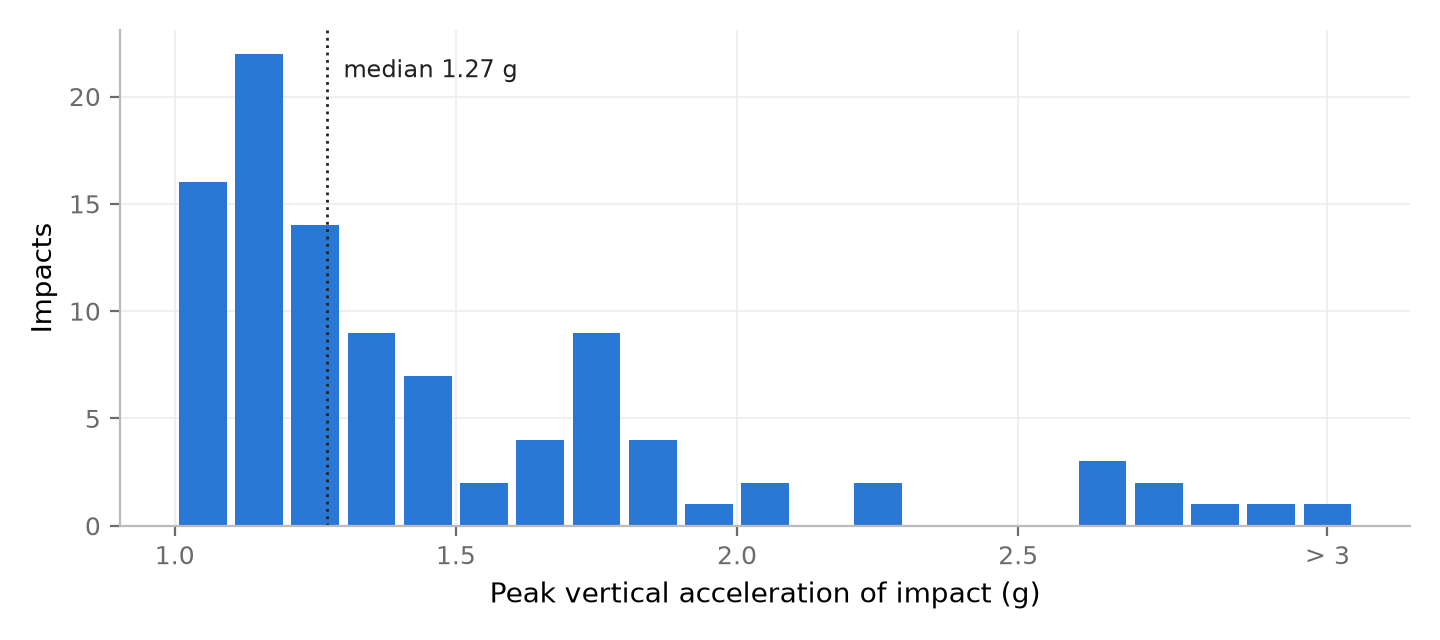
\includegraphics[width=\linewidth]{fig_a2_severity.png}}
\caption{Peak vertical acceleration of the 100 impacts from all three rides. The
detection threshold is 1.0 g; impacts above 3 g are shown as one bar
(one impact, 6.28 g).}\label{fig:2}
\end{figure}

Rates differed between rides (12.3--26.4 per km). Ride 2's higher rate comes largely
from one stretch where 13 impacts followed each other every 0.6--1.2 s at about 8 km/h
over roughly 20 m; ride 3 also produced a cluster there (spot P3, Table~\ref{tab:3}). Whether
this is a rough surface, such as setts or a broken patch, has not yet been checked.

\textbf{Speed and severity.} In ride 1 the impact peak was not related to speed (Spearman
ρ = 0.03, p = 0.88 \autocite{spearman1904}). In rides 2 and 3, slower impacts were stronger
(ρ = −0.63 and −0.68), and pooled ρ = −0.48. This pooled association comes mostly from
the two dense clusters at about 8 km/h (Figure~\ref{fig:speed}): without the spots of 10
or more impacts, ρ = −0.12 (p = 0.33, n = 71), and with one value per spot, ρ = −0.36
(p = 0.04, n = 33). Because impacts within a spot are not independent, these p-values
overstate the evidence; no conclusion about speed is drawn.

% paper/figures/fig_a5_speed.png (scripts/paper_part_a.py, fig_speed)
\begin{figure}
\centering
{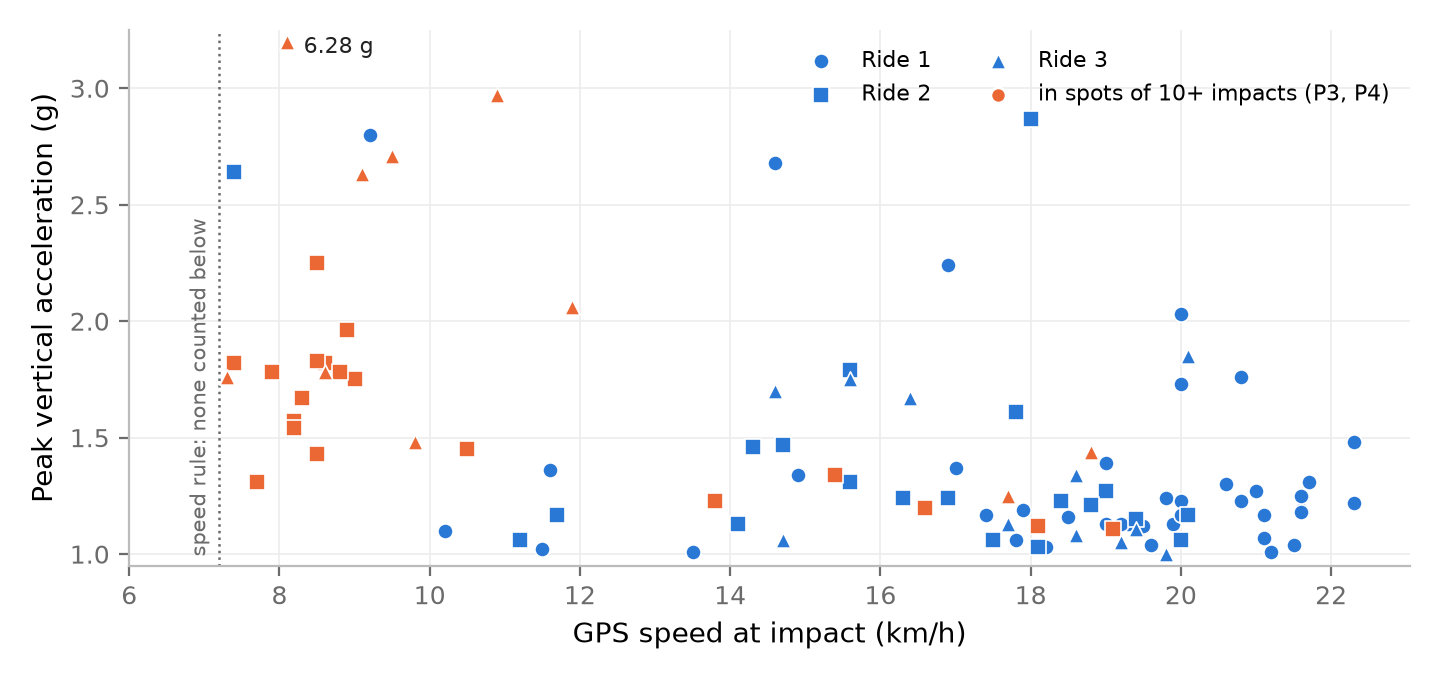
\includegraphics[width=\linewidth]{fig_a5_speed.png}}
\caption{GPS speed at impact against peak vertical acceleration, all 100 impacts (marker
shape: ride). Orange: the 29 impacts in the two spots with 10 or more impacts (P3, P4,
Table~\ref{tab:3}), which produce most of the pooled speed--severity association. The
6.28 g impact is drawn at the top edge. Dotted line: speed rule (7.2 km/h); impacts at
lower speeds are not counted.}\label{fig:speed}
\end{figure}

\subsubsection{Where the impacts were}\label{where-the-impacts-were}

% outputs/combined/by_road.csv

Per km ridden, the study roads gave 12.3 impacts (Marston Road, 2.52 km), 14.3 (Morrell
Avenue, 1.05 km) and 8.3 (Old Road, 0.24 km), and other roads 22.7 (2.25 km)
(Figure~\ref{fig:3}). Headington Road was ridden for only 0.02 km, too little for a rate.

\begin{figure}
\centering
{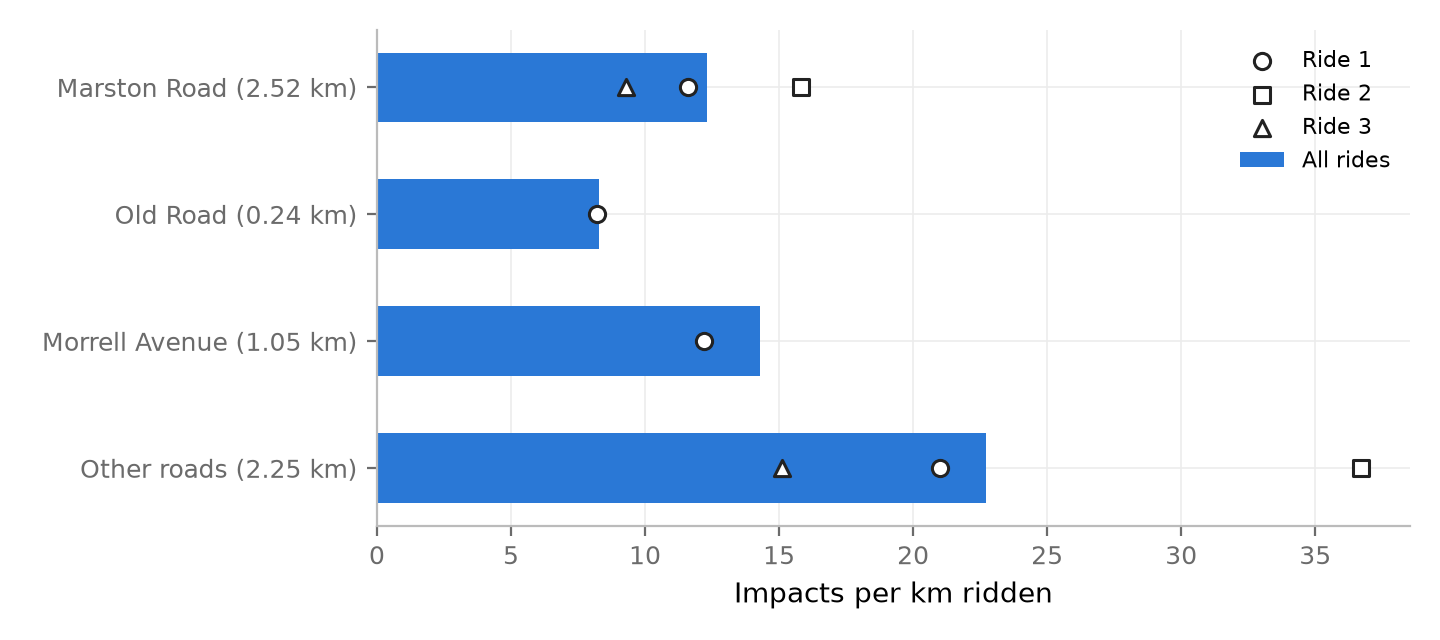
\includegraphics[width=\linewidth]{fig_a3_roads.png}}
\caption{Impacts per km ridden by road, all rides (bars) and per ride (markers).
Rates are shown only where at least 0.2 km was ridden on the road by that ride; the
distance ridden on each road over all rides is given in brackets.}\label{fig:3}
\end{figure}

% outputs/combined/spot_links.csv; part_a_numbers.json: spots

The impacts formed 33 spots: \textbf{10 hit on two or more separate rides}, 10 with several
impacts from one ride, and 13 single impacts (Figure~\ref{fig:4}). Two spots on Marston Road, P1
and P2, were hit on all three rides (Table~\ref{tab:3}). The strongest single impact, 6.28 g, lies
in spot P4, which was hit on two rides.

\begin{figure}
\centering
{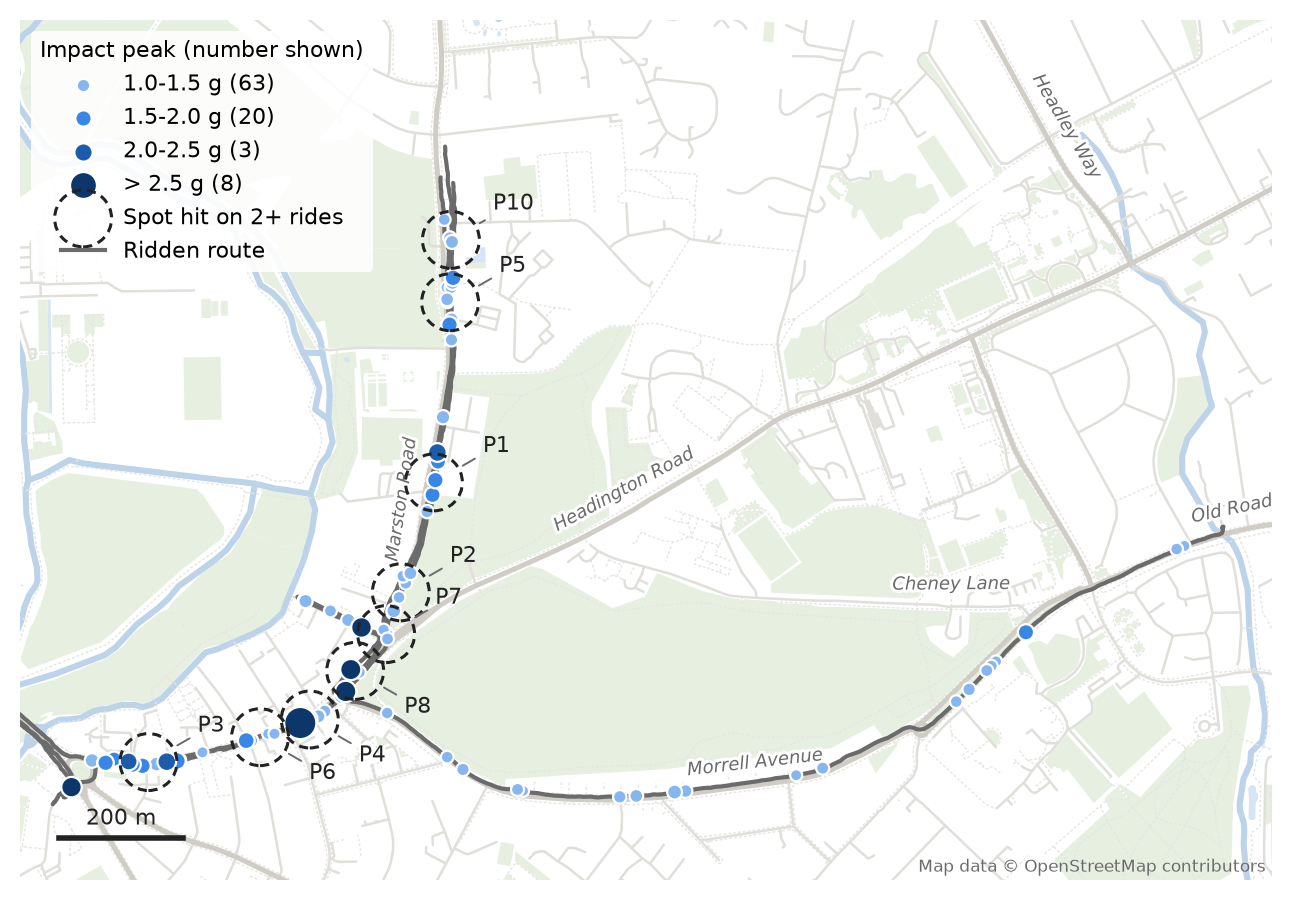
\includegraphics[width=\linewidth]{fig_a4_map.png}}
\caption{Impacts from all three rides on the ridden routes, coloured and sized by peak
vertical acceleration; dashed circles mark the 10 spots hit on two or more rides
(Table~\ref{tab:3}). For privacy, the first and last 200 m of each route are not drawn; the 6
impacts in those parts are included in all statistics. Background: streets, paths, parks and
water from OpenStreetMap \autocite{osm}, map data \textcopyright{} OpenStreetMap contributors (ODbL).}\label{fig:4}
\end{figure}

\begin{longtable}[]{@{}
  >{\raggedright\arraybackslash}p{(\linewidth - 12\tabcolsep) * \real{0.1429}}
  >{\raggedright\arraybackslash}p{(\linewidth - 12\tabcolsep) * \real{0.1429}}
  >{\raggedright\arraybackslash}p{(\linewidth - 12\tabcolsep) * \real{0.1429}}
  >{\raggedright\arraybackslash}p{(\linewidth - 12\tabcolsep) * \real{0.1429}}
  >{\raggedright\arraybackslash}p{(\linewidth - 12\tabcolsep) * \real{0.1429}}
  >{\raggedright\arraybackslash}p{(\linewidth - 12\tabcolsep) * \real{0.1429}}
  >{\raggedright\arraybackslash}p{(\linewidth - 12\tabcolsep) * \real{0.1429}}@{}}
\caption{Spots hit on two or more rides, with the nearest FixMyStreet road-surface report made in the 365 days before the ride.}\label{tab:3}\tabularnewline
\toprule\noalign{}
\begin{minipage}[b]{\linewidth}\raggedright
Spot
\end{minipage} & \begin{minipage}[b]{\linewidth}\raggedright
Rides
\end{minipage} & \begin{minipage}[b]{\linewidth}\raggedright
Impacts
\end{minipage} & \begin{minipage}[b]{\linewidth}\raggedright
Max (g)
\end{minipage} & \begin{minipage}[b]{\linewidth}\raggedright
Road
\end{minipage} & \begin{minipage}[b]{\linewidth}\raggedright
Recent report within 25 m
\end{minipage} & \begin{minipage}[b]{\linewidth}\raggedright
Nearest recent report
\end{minipage} \\
\midrule\noalign{}
\endfirsthead
\toprule\noalign{}
\begin{minipage}[b]{\linewidth}\raggedright
Spot
\end{minipage} & \begin{minipage}[b]{\linewidth}\raggedright
Rides
\end{minipage} & \begin{minipage}[b]{\linewidth}\raggedright
Impacts
\end{minipage} & \begin{minipage}[b]{\linewidth}\raggedright
Max (g)
\end{minipage} & \begin{minipage}[b]{\linewidth}\raggedright
Road
\end{minipage} & \begin{minipage}[b]{\linewidth}\raggedright
Recent report within 25 m
\end{minipage} & \begin{minipage}[b]{\linewidth}\raggedright
Nearest recent report
\end{minipage} \\
\midrule\noalign{}
\endhead
\bottomrule\noalign{}
\endlastfoot
P1 & 3 & 6 & 2.24 & Marston Road & No & 60 m (closed) \\
P2 & 3 & 6 & 1.47 & Marston Road & No & 44 m (closed) \\
P3 & 2 & 19 & 2.25 & Other & Yes & 5 m (closed) \\
P4 & 2 & 10 & 6.28 & Other & Yes & 8 m (fixed) \\
P5 & 2 & 9 & 1.79 & Marston Road & No & 121 m (closed) \\
P6 & 2 & 4 & 1.85 & Other & Yes & 8 m (closed) \\
P7 & 2 & 3 & 1.17 & Marston Road & Yes & 8 m (closed) \\
P8 & 2 & 2 & 2.80 & Other & No & 38 m (closed) \\
P9 & 2 & 2 & 2.03 & Marston Road & No & 125 m (fixed) \\
P10 & 2 & 2 & 1.34 & Marston Road & No & 87 m (closed) \\
\end{longtable}

\subsubsection{Comparison with FixMyStreet}\label{comparison-with-fixmystreet-1}

% outputs/recordings/<rec>/fms_match_rates.csv

At the level of single impacts, FixMyStreet reports did not single out the places where
impacts occurred. A recent report lay within 25 m of 2 of 40 impacts in ride 1 (5\%,
route baseline 14\%), 12 of 39 in ride 2 (31\%, baseline 33\%) and 9 of 21 in ride 3
(43\%, baseline 34\%): close to what chance would give in each ride. At the level of
spots, 6 of the 10 spots hit on two or more rides had no recent report within 25 m,
including both spots hit on all three rides (Table~\ref{tab:3}). Spot P4, with the 6.28 g impact,
had a report within 8 m marked ``fixed''; its report and repair dates have not been
checked. A missing FixMyStreet report does not mean that a defect was unknown to the
highway authority, which also receives reports through other channels and inspects
roads itself.

\textbf{Visual check.} The spots are being checked in street-level imagery with rules fixed
in advance (Appendix C); results are pending.

% TODO: fill in from outputs/combined/spot_links.csv (imagery_date, what_visible)

\subsubsection{Summary of Part A}\label{summary-of-part-a}

Riding three Voiager 5 scooters over 6.08 km produced 100 jolts of 1 g or more at the
handlebar, about one every 61 m, a third of them 1.5 g or more. Ten places produced
impacts on two or more separate rides, and most of these had no recent public report.
These results come from one rider, one phone and short routes, and use analyst-chosen
thresholds; they describe exposure on these rides, not the risk to riders in general.

% Converted from part_b_methods_results.md by scripts/md_to_latex.py; edit this file.
% DRAFT v0.1 (2026-10-07). Part B of the paper: wheel-size models, methods and results.
% Citations use Pandoc keys from ../references.bib, e.g. [@posirisuk2022].
% Build later with: pandoc part_b_methods_results.md --citeproc --bibliography ../references.bib -o part_b.docx
% Every number below is taken from outputs/ (paths given in the HTML comments) or from
% SIMULATION_METHODS.md. Re-check them if any simulation is rerun.
% Wheel sizes for the Voiager 5 are the reported 10/10 (stated assumption; see DOCUMENTATION.md 12).

\section{Methods: modelling the effect of wheel size}\label{methods-modelling-the-effect-of-wheel-size}

\subsection{Overview}\label{overview}

Rental e-scooters are the only e-scooters that may legally be ridden on UK public roads,
so a scooter with modified wheels cannot be tested on the road. We therefore used two
models, in the same way as the Imperial College study of e-scooter falls this work builds
on \autocite{posirisuk2022}:

\begin{enumerate}
\def\labelenumi{\arabic{enumi}.}
\tightlist
\item
  a \textbf{geometry model}, which describes how far a single wheel drops into a pothole and
  how hard it strikes the far edge, and
\item
  a \textbf{planar multibody dynamics model} of scooter and rider in MuJoCo
  \autocite{todorov2012mujoco}, which predicts whether the scooter pitches over.
\end{enumerate}

Both models compare wheel configurations under identical assumptions. They are not
validated against physical tests, so we report relative differences between
configurations, not real-world fall thresholds.

\subsection{Wheel configurations}\label{wheel-configurations}

Configurations are written front/rear diameter in inches (nominal size taken as tyre
outer diameter).

{\def\LTcaptype{none} % do not increment counter
\begin{longtable}[]{@{}
  >{\raggedright\arraybackslash}p{(\linewidth - 2\tabcolsep) * \real{0.5000}}
  >{\raggedright\arraybackslash}p{(\linewidth - 2\tabcolsep) * \real{0.5000}}@{}}
\toprule\noalign{}
\begin{minipage}[b]{\linewidth}\raggedright
Configuration
\end{minipage} & \begin{minipage}[b]{\linewidth}\raggedright
Meaning
\end{minipage} \\
\midrule\noalign{}
\endhead
\bottomrule\noalign{}
\endlastfoot
10/10 & Current vehicle (Voi Voiager 5, the model of all three ridden scooters as confirmed by Voi customer support \autocite{voi2026support_rec01,voi2026support_rec0203}), using the reported 10 in wheel size \autocite{levy_voiager5,alsalkini2023}; the front/rear split is not published, so equal wheels are assumed \\
12/10 & Larger front wheel only, as on Voi's Voiager 7 (12 in front) \autocite{startups2024voiager7} \\
12/12 & Larger wheels front and rear \\
14/10 & Much larger front wheel only \\
\end{longtable}
}

A front/rear ratio study added 16/10, 20/10, 16/8 and 20/8 (ratios up to 2.5).

\subsection{Geometry model}\label{geometry-model}

A rigid wheel of radius \(R\) rolls at speed \(v\) across a rectangular pothole of depth \(d\)
and length \(w\) with sharp edges. The wheel's lowest point sinks below road level by

\[h = \min\left(d,\; R - \sqrt{R^2 - (w/2)^2},\; \tfrac{1}{2} g \left(\tfrac{w}{v}\right)^2\right),\]

the smallest of the depth, the sag of a wheel resting on both edges, and the free-fall
distance in the time taken to cross (an upper bound). The far edge then meets the tyre at
an angle \(\theta\) from vertical, with \(\cos\theta = (R-h)/R\). Treating the impact as
plastic, the velocity lost into the edge is \(v\sin\theta\) and the forward speed loss of
the axle is \(v\sin^2\theta\). A larger wheel gives a smaller \(\theta\) for the same pothole,
so both quantities fall. Each wheel is analysed separately, so this model cannot say
whether the scooter falls; that requires the dynamics model.

The geometry model was evaluated for 8--16 in wheels, speeds of 15, 20 and 25 km/h,
depths of 0--120 mm and lengths of 150--1000 mm (\texttt{scripts/wheel\_geometry.py}).

\subsection{Dynamics model}\label{dynamics-model}

\textbf{Structure.} The model is planar (side view) with six degrees of freedom: forward
position, height and pitch of the chassis; rotation of each wheel; and forward lean of
the rider. It follows the structure of \textcite{posirisuk2022}, who modelled the scooter as the
front wheel and the rest of the scooter joined at the axle, but adds a separate rear
wheel, so that front-only and front-and-rear changes can be compared, and a rider. The
rider is a single rigid body pinned to the deck at the feet; a rotational spring
(1500 N·m/rad) and damper (150 N·m·s/rad) represent the rider bracing with legs and arms,
chosen so that braking at 0.3 g leans the rider about 8° forward.

\textbf{Parameters.} Voi does not publish the vehicle's mass properties, so most parameters
are assumed (Table~\ref{tab:4}). The rider's mass and height match the median male model of
\textcite{posirisuk2022}.

\begin{longtable}[]{@{}
  >{\raggedright\arraybackslash}p{(\linewidth - 4\tabcolsep) * \real{0.3333}}
  >{\raggedright\arraybackslash}p{(\linewidth - 4\tabcolsep) * \real{0.3333}}
  >{\raggedright\arraybackslash}p{(\linewidth - 4\tabcolsep) * \real{0.3333}}@{}}
\caption{Main model parameters.}\label{tab:4}\tabularnewline
\toprule\noalign{}
\begin{minipage}[b]{\linewidth}\raggedright
Parameter
\end{minipage} & \begin{minipage}[b]{\linewidth}\raggedright
Value
\end{minipage} & \begin{minipage}[b]{\linewidth}\raggedright
Source
\end{minipage} \\
\midrule\noalign{}
\endfirsthead
\toprule\noalign{}
\begin{minipage}[b]{\linewidth}\raggedright
Parameter
\end{minipage} & \begin{minipage}[b]{\linewidth}\raggedright
Value
\end{minipage} & \begin{minipage}[b]{\linewidth}\raggedright
Source
\end{minipage} \\
\midrule\noalign{}
\endhead
\bottomrule\noalign{}
\endlastfoot
Scooter mass & 32 kg & Assumed (Voiager 7 reported at 36 kg \autocite{startups2024voiager7}) \\
Wheel mass & 2.5 kg each & Assumed; scaling with diameter did not change results \\
Wheelbase & 0.95 m & Assumed \\
Deck height & 0.16 m (10 in wheels), rising with wheel size; deck kept level & Assumed \\
Handlebar height & 1.05 m & Assumed \\
Rider & 76 kg, 1.70 m, centre of mass at 55\% of height & \textcite{posirisuk2022}; centre-of-mass fraction assumed \\
Tyre compliance & Contact time constant 0.025 s (≈80 kN/m, ≈6 mm static deflection) & Assumed, typical small pneumatic tyre \\
Front fork & 25 kN/m, damping ratio 0.3, 30 mm travel & Assumed; the Voiager 5 has a front spring \autocite{levy_voiager5} \\
Friction & 0.9 & Dry asphalt, assumed \\
Integration & Implicit-fast, 0.5 ms time step & Numerical choice \\
\end{longtable}

\textbf{Tyre contact.} Wheels are rigid cylinders whose contact with the road is softened
through MuJoCo's soft-contact parameters to represent tyre compliance.

\textbf{Front suspension.} Because the Voiager 5 has a front spring, the main results use a
sprung front fork (Table~\ref{tab:4}). Its values were fixed before any run and tested in the
sensitivity analysis. Results without suspension are reported for comparison.

\textbf{Pothole.} The main experiments use a rectangular pothole with vertical walls and sharp
edges, 5 m after the start, giving about 1 s of run-up. To test potholes with broken
edges, a second contact model computes tyre--road contact directly against a sampled road
profile in which each edge falls over a width \(b\) with a raised-cosine shape (0, 25, 50 or
100 mm). It applies one radial spring-damper force per wheel. Before use, it was checked
on a flat road (0.01 g at the handlebar), for convergence with profile resolution, and
against MuJoCo's own contact on sharp edges, where fall outcomes agreed in 30 of 30 cases.
Its absolute accelerations are too high because a point contact cannot envelop an edge,
so it is used only to compare falls between edge shapes.

\textbf{Procedure.} Each run settles the model at rest for 0.5 s, sets the forward speed and
matching wheel spin, and lets the scooter coast (no motor or braking, no steering)
across the pothole.

\textbf{Outcomes.} Speed loss, maximum scooter pitch and rider lean, and peak acceleration at
the handlebar, where the phone was mounted. The handlebar acceleration is averaged over
10 ms windows to match the phone's 100 Hz sampling.

\textbf{Fall definition.} A run counts as a fall if the rider leans more than 30° forward,
the scooter pitches more than 30° nose-down, or forward speed drops below 0.5 m/s. These
thresholds are analyst-defined and were fixed before any experiment. A fall is attributed
to the rear wheel only if the rear wheel dipped more than 5 mm into the pothole before
the fall; otherwise it is attributed to the front-wheel impact.

\subsection{Experiments}\label{experiments}

\begin{longtable}[]{@{}
  >{\raggedright\arraybackslash}p{(\linewidth - 4\tabcolsep) * \real{0.3333}}
  >{\raggedright\arraybackslash}p{(\linewidth - 4\tabcolsep) * \real{0.3333}}
  >{\raggedright\arraybackslash}p{(\linewidth - 4\tabcolsep) * \real{0.3333}}@{}}
\caption{Simulation experiments.}\label{tab:5}\tabularnewline
\toprule\noalign{}
\begin{minipage}[b]{\linewidth}\raggedright
Experiment
\end{minipage} & \begin{minipage}[b]{\linewidth}\raggedright
Design
\end{minipage} & \begin{minipage}[b]{\linewidth}\raggedright
Runs
\end{minipage} \\
\midrule\noalign{}
\endfirsthead
\toprule\noalign{}
\begin{minipage}[b]{\linewidth}\raggedright
Experiment
\end{minipage} & \begin{minipage}[b]{\linewidth}\raggedright
Design
\end{minipage} & \begin{minipage}[b]{\linewidth}\raggedright
Runs
\end{minipage} \\
\midrule\noalign{}
\endhead
\bottomrule\noalign{}
\endlastfoot
Main sweep & 4 configurations × 9 depths (20--100 mm) × 3 lengths (300, 600, 1000 mm) × 3 speeds (15, 20, 25 km/h); with and without front suspension & 324 each \\
Sensitivity & Tyre stiffness (τ = 0.015, 0.035 s), rider bracing (1000, 3000 N·m/rad) and, with suspension, fork stiffness (15, 40 kN/m) and damping (ratio 0.15, 0.5), varied one at a time & 5 settings (9 with suspension) × 4 configurations \\
Front/rear ratio & 7 configurations from 10/10 to 20/8 on the main grid & 567 each \\
Soft edges & Profile contact with suspension; edge widths 0, 25, 50, 100 mm × main sweep & 1296 \\
Consistency check & 10/10 at 20 km/h on assumed common potholes (20--40 mm deep, 300 and 600 mm long) & 6 per model (with and without suspension) \\
\end{longtable}

The depth grid has a 10 mm resolution, so a reported threshold of ``80 mm'' means a first
fall somewhere between 70 and 80 mm. All runs are deterministic; rerunning the main sweep
and sensitivity analysis reproduced every outcome exactly. Analysis used NumPy, pandas
and Matplotlib \autocite{harris2020numpy,mckinney2010pandas,hunter2007matplotlib}; animations
were drawn with Matplotlib and encoded with Pillow \autocite{pillow}.

\textbf{Consistency check.} The criterion, fixed before running, was that simulated
handlebar peaks for the current scooter on common potholes should fall within roughly
1--3 g, the range of the measured impacts. With the three rides of Part A, 99 of 100
measured peaks were 1.0--2.97 g (median 1.27 g) and one was 6.28 g; the first ride alone
gave 1.0--2.8 g. Pothole depths along the route were not measured, so this is a
consistency check, not a validation.

\section{Results: what a larger front wheel would change}\label{results-what-a-larger-front-wheel-would-change}

\subsection{Geometry}\label{geometry}

At 20 km/h on a 600 mm long pothole, a 12 in front wheel reduced the edge impact
velocity by 6.5--7.7\% and the front-wheel speed loss by 12.6--14.8\% compared with a 10 in
wheel; a 14 in wheel reduced them by 12.1--13.9\% and 22.6--25.8\% (Table~\ref{tab:6}). At speed, wheels barely dropped
into short potholes (about 3 mm into a 150 mm pothole at 20 km/h), so long potholes are
the more dangerous ones.

% outputs/wheel_model/configurations.csv

\begin{longtable}[]{@{}
  >{\raggedright\arraybackslash}p{(\linewidth - 4\tabcolsep) * \real{0.3333}}
  >{\raggedright\arraybackslash}p{(\linewidth - 4\tabcolsep) * \real{0.3333}}
  >{\raggedright\arraybackslash}p{(\linewidth - 4\tabcolsep) * \real{0.3333}}@{}}
\caption{Front-wheel edge impact at 20 km/h, 600 mm pothole (geometry model).}\label{tab:6}\tabularnewline
\toprule\noalign{}
\begin{minipage}[b]{\linewidth}\raggedright
Front wheel
\end{minipage} & \begin{minipage}[b]{\linewidth}\raggedright
Depth 30 mm: impact velocity / speed loss
\end{minipage} & \begin{minipage}[b]{\linewidth}\raggedright
Depth 60 mm: impact velocity / speed loss
\end{minipage} \\
\midrule\noalign{}
\endfirsthead
\toprule\noalign{}
\begin{minipage}[b]{\linewidth}\raggedright
Front wheel
\end{minipage} & \begin{minipage}[b]{\linewidth}\raggedright
Depth 30 mm: impact velocity / speed loss
\end{minipage} & \begin{minipage}[b]{\linewidth}\raggedright
Depth 60 mm: impact velocity / speed loss
\end{minipage} \\
\midrule\noalign{}
\endhead
\bottomrule\noalign{}
\endlastfoot
10 in & 3.59 m/s / 41.7\% & 4.64 m/s / 69.8\% \\
12 in & 3.31 m/s / 35.5\% (−7.7\% / −14.8\%) & 4.34 m/s / 61.0\% (−6.5\% / −12.6\%) \\
14 in & 3.09 m/s / 30.9\% (−13.9\% / −25.8\%) & 4.08 m/s / 54.0\% (−12.1\% / −22.6\%) \\
\end{longtable}

At 60 mm and deeper, the drop is limited by the time available to fall (57 mm), so the
60 and 90 mm results are identical.

\begin{figure}[htbp]
\centering
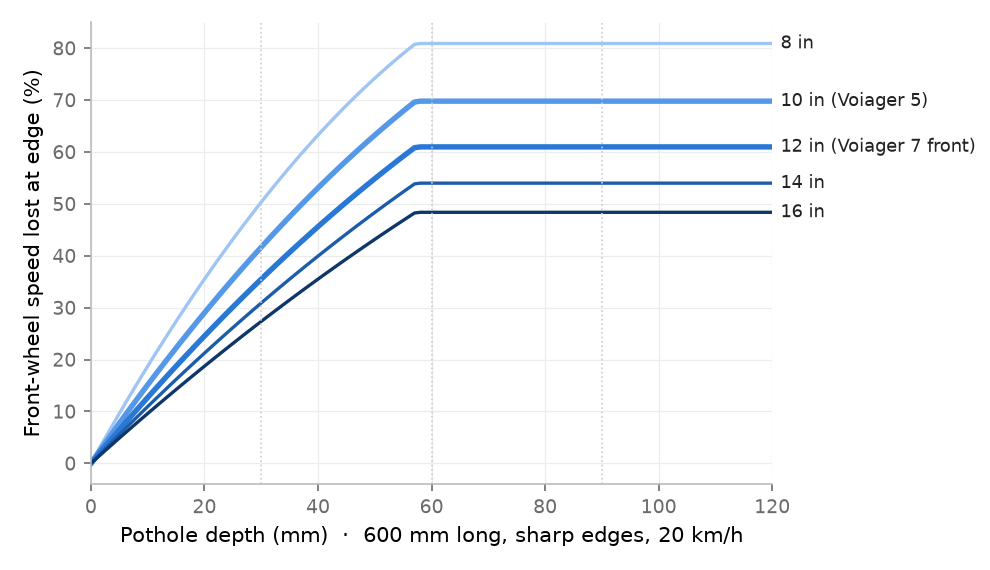
\includegraphics[width=\linewidth]{sim/geom_speed_loss.png}
\caption{Geometry model: share of the front wheel's speed lost at the far edge of a 600 mm long, sharp-edged pothole at 20 km/h, by wheel diameter. Rigid wheel, no tyre or suspension; the curves flatten at 57 mm, the deepest the wheel can drop in the time available. Schematic and further geometry results in Appendix~\ref{app:model}.}\label{fig:geom}
\end{figure}

Figure~\ref{fig:geom} shows the same comparison over all depths.

\subsection{Falls with the Voiager 5's front suspension}\label{falls-with-the-voiager-5s-front-suspension}

% outputs/scooter_sim/suspension/sim_results.csv, fall_thresholds.csv

With front suspension, falls occurred in 9 of 81 runs for the current 10/10
configuration, 6 for 12/10, 6 for 12/12 and 1 for 14/10 (Table~\ref{tab:7}). No 300 mm long
pothole caused a fall at any depth up to 100 mm; 600 mm potholes caused falls only at
15 km/h, where the slower wheel has more time to drop.

\begin{longtable}[]{@{}lllll@{}}
\caption{Shallowest pothole depth (mm) causing a fall, with front suspension (-- = no fall up to 100 mm). Rows with no falls in any configuration are omitted.}\label{tab:7}\tabularnewline
\toprule\noalign{}
Length, speed & 10/10 & 12/10 & 12/12 & 14/10 \\
\midrule\noalign{}
\endfirsthead
\toprule\noalign{}
Length, speed & 10/10 & 12/10 & 12/12 & 14/10 \\
\midrule\noalign{}
\endhead
\bottomrule\noalign{}
\endlastfoot
600 mm, 15 km/h & 80 & 90 & 90 & -- \\
1000 mm, 15 km/h & 90 & 100 & 100 & -- \\
1000 mm, 20 km/h & 90 & 90 & 90 & 100 \\
1000 mm, 25 km/h & 90 & 100 & 100 & -- \\
\textbf{Falls (of 81 runs)} & \textbf{9} & \textbf{6} & \textbf{6} & \textbf{1} \\
\end{longtable}

% outputs/scooter_sim/keyframes/keyframes_runs.csv

Figure~\ref{fig:5} shows one such case as still frames: the 80 mm deep, 600 mm long pothole at
15 km/h, the shallowest falling depth for the current scooter (Table~\ref{tab:7}). With 10 in
wheels the front wheel drops into the hole and strikes the far edge, and the scooter
pitches forward about it; the fall criterion is reached 0.15 s after the front wheel
reaches the edge. With a 12 in front wheel, alone or with a 12 in rear wheel, the
scooter rolls out with almost identical motion (maximum chassis pitch 13--14°,
speed loss 71--72\%). With a 14 in front wheel it rolls out with less pitch
(7°) and less speed loss (56\%).

\begin{figure}
\centering
{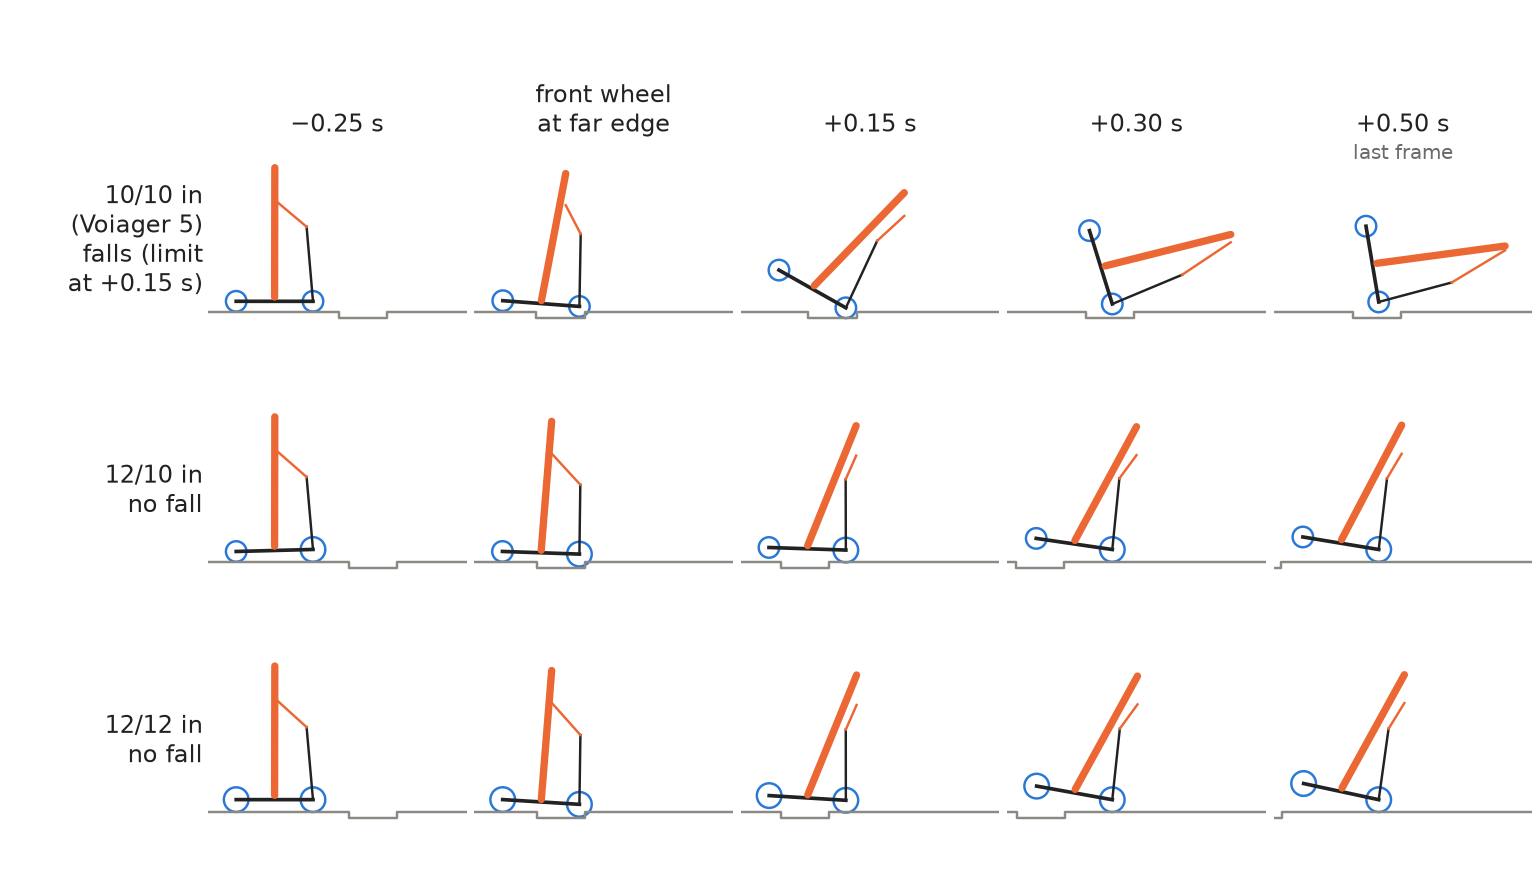
\includegraphics[width=\linewidth]{fig_b5_keyframes_sharp.png}}
\caption{Key frames from the simulation of the Voiager 5 model with its front spring
crossing a sharp-edged pothole 80 mm deep and 600 mm long at 15 km/h. Rows: wheel
configuration (front/rear diameter). Columns: the same moments in each row, relative to
the front wheel reaching the pothole's far edge; the view follows the front wheel. Blue:
wheels; black: deck and stem; orange: rider. The rider is pinned to the deck at the
feet, so scooter and rider rotate together; a real rider would separate from the scooter.
Planar model with assumed parameters (Table~\ref{tab:4}); one run per configuration, illustrating
the results of Table~\ref{tab:7}.}\label{fig:5}
\end{figure}

Every fall in every configuration was a forward pitch-over of scooter and rider about the
front wheel, started by the front-wheel impact; the rear wheel was lifted clear and never
entered the pothole before a fall. This matches the mechanism reported by
\textcite{posirisuk2022}.

The benefit of a 12 in front wheel was modest with suspension: it delayed the first fall
by 10 mm in three of the four cases above, and speed loss on a 60 × 600 mm pothole at
20 km/h was 25.5\% against 27.6\% for 10/10. A 14 in front wheel almost eliminated falls in
the tested range.

Without suspension, falls were more frequent (15, 14, 14 and 11 of 81 runs for 10/10,
12/10, 12/12 and 14/10), began at 70--80 mm for the current scooter, and the 12 in front
wheel delayed the fall by 10 mm on a 1000 mm pothole at 20 km/h (70 → 80 mm). The front
suspension itself therefore had a large effect, comparable to enlarging the front wheel.

\subsection{A larger front wheel alone performs like larger wheels front and rear}\label{a-larger-front-wheel-alone-performs-like-larger-wheels-front-and-rear}

The central comparison of the hypothesis is 12/10 against 12/12. In the main sweep they
had the same number of falls and the same shallowest falling depth in every case, both
with suspension (Table~\ref{tab:7}) and without. The reason is visible in the simulations: with
10--12 in wheels, the front-edge impact lifts the rear of the scooter so that the rear
wheel skips over the pothole, so its size makes almost no difference to whether the
scooter falls. In Figure~\ref{fig:5} the 12/10 and 12/12 rows are almost indistinguishable (speed
loss 70.9\% and 71.7\%).

\subsection{Sensitivity}\label{sensitivity}

% outputs/scooter_sim/sensitivity.csv, outputs/scooter_sim/suspension/sensitivity.csv

Without suspension, the 12/10 configuration fell at the same depth as 12/12, and 10 mm
deeper than 10/10, under all five tyre and bracing settings; the current scooter's
first fall on a 1000 mm pothole at 20 km/h moved between 60 and 70 mm with tyre
stiffness. With suspension, 12/10 and 12/12 fell at the same depth in 8 of 9 settings
(the exception, more fork damping, differed by 10 mm). The ordering of configurations was
therefore robust, but absolute fall depths depend on assumed parameters and should not be
read as real-world thresholds.

\subsection{Potholes without sharp edges}\label{potholes-without-sharp-edges}

% outputs/scooter_sim/suspension/soft_edges/edge_fall_counts.csv

\begin{longtable}[]{@{}lllll@{}}
\caption{Number of falls (of 81 runs) by edge width, profile contact with suspension.}\label{tab:8}\tabularnewline
\toprule\noalign{}
Edge width & 10/10 & 12/10 & 12/12 & 14/10 \\
\midrule\noalign{}
\endfirsthead
\toprule\noalign{}
Edge width & 10/10 & 12/10 & 12/12 & 14/10 \\
\midrule\noalign{}
\endhead
\bottomrule\noalign{}
\endlastfoot
0 mm (sharp) & 8 & 6 & 6 & 4 \\
25 mm & 8 & 5 & 6 & 4 \\
50 mm & 7 & 5 & 5 & 4 \\
100 mm & 4 & 3 & 3 & 2 \\
\end{longtable}

Sloped edges reduced falls (10/10: 8 to 4 from sharp to 100 mm edges). At every edge
width, the configurations with a larger front wheel fell less often than the current
scooter, and 12/10 stayed within one fall of 12/12. Figure~\ref{fig:6} shows the same 80 × 600 mm
pothole with 50 mm sloped edges: the current scooter still pitches over, more slowly
(fall criterion at 0.42 s), while 12 in and 14 in front wheels roll through. As with
sharp edges, 12/10 and 12/12 move almost identically (maximum chassis pitch 16°, speed
loss 50\%); 14/10 pitches less (11°, speed loss 44\%).

\begin{figure}
\centering
{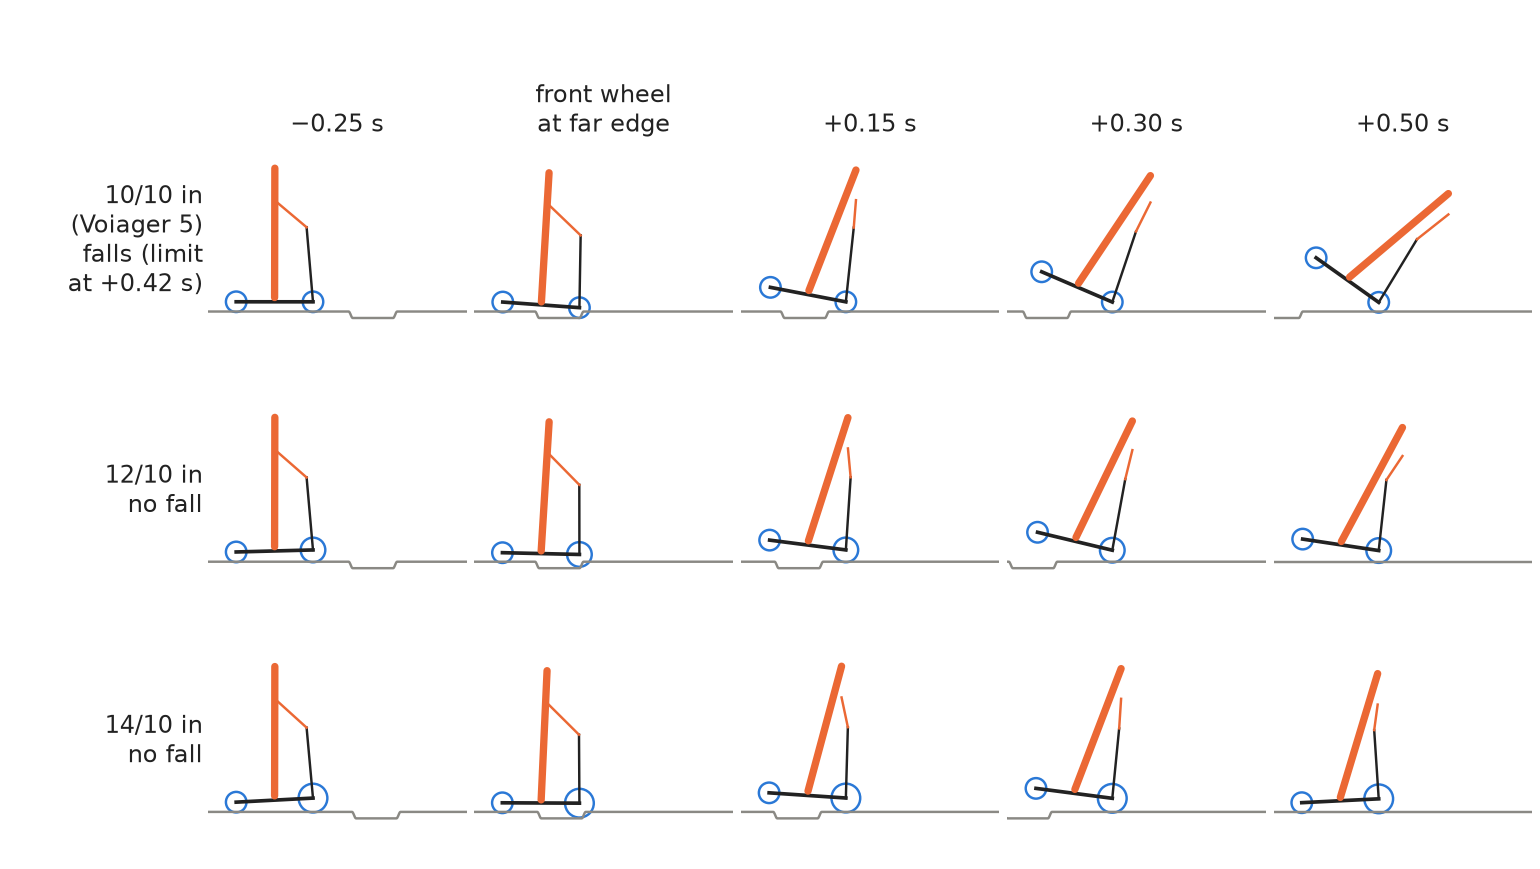
\includegraphics[width=\linewidth]{fig_b6_keyframes_edge50.png}}
\caption{As Figure~\ref{fig:5}, but each pothole edge slopes over 50 mm (raised-cosine profile,
custom tyre contact; section 3.4). Jolt sizes from
this contact model are not used as results; fall outcomes are.}\label{fig:6}
\end{figure}

\subsection{How much larger should the front wheel be?}\label{how-much-larger-should-the-front-wheel-be}

% outputs/scooter_sim/ratio/, outputs/scooter_sim/suspension/ratio/

The ratio study asked whether a front wheel can be too large relative to the rear. It
repeated the main sweep (81 runs per configuration) for front/rear diameter ratios from
1.0 (10/10) to 2.5 (20/8); the full results are in Appendix~\ref{app:ratio}. Falls kept
decreasing as the front wheel grew (Table~\ref{tab:9}): from 15 of 81 runs for 10/10 to 1
for 20/10 and 20/8 without suspension, and from 9 to none with suspension. No ratio up
to 2.5 made falls more likely: with a larger front wheel the shallowest depth causing a
fall stayed the same or rose, in 10 mm steps (Figures~\ref{fig:Eratiofork} and~\ref{fig:Erationofork}).

% outputs/scooter_sim/ratio/ratio_results.csv, outputs/scooter_sim/suspension/ratio/ratio_results.csv
\begin{table}[htbp]
\centering\small
\caption{Front/rear ratio study: runs meeting the fall criteria (of 81 per configuration). Planar model with assumed parameters (Table~\ref{tab:4}); relative comparison of wheel configurations only.}\label{tab:9}
\begin{tabular}{@{}lrrr@{}}
\toprule
Front/rear (in) & Ratio & Without suspension & With suspension \\
\midrule
10/10 & 1.0 & 15 & 9 \\
11/10 & 1.1 & 15 & 9 \\
12/10 & 1.2 & 14 & 6 \\
14/10 & 1.4 & 11 & 1 \\
16/10 & 1.6 & 9 & 1 \\
20/10 & 2.0 & 1 & 0 \\
16/8 & 2.0 & 9 & 1 \\
20/8 & 2.5 & 1 & 0 \\
\bottomrule
\end{tabular}
\end{table}


Very large front wheels did change what the rear wheel does (Figures~\ref{fig:Erearfork}
and~\ref{fig:Erearnofork}). With a small front wheel, the front impact lifts the rear so
that it skips over the pothole. With a very large front wheel it no longer does, so the
rear wheel drops into the pothole and causes a second jolt: without suspension, the
largest speed loss at the rear crossing (20 km/h, runs without a fall) rose from 19\% for
10/10 to 27\% for 20/10 and 33\% for 20/8. With suspension the configurations differed
little. This second jolt caused no falls in the model, but it would affect comfort and
control.

In this model a larger front wheel was never worse: falls kept decreasing up to the
largest front wheel tested (20 in). With front suspension, however, most of the reduction
was reached by 14/10 (from 9 to 1 of 81 runs), and larger front wheels added little. The
model cannot represent steering, frame geometry, weight or cost, all of which limit how
large a front wheel can practically be, and the rear-wheel jolt above would affect
comfort. We therefore suggest a moderate increase (12--14 in), in line with wheels already
in use: the Voiager 7 has a 12 in front wheel \autocite{startups2024voiager7}, and London's
tender requires a front wheel of at least 11 in \autocite{tfl2022tender}. This limit is a
judgement based on factors outside the model, not a result of it.

\subsection{Consistency with the measured rides}\label{consistency-with-the-measured-rides}

% outputs/scooter_sim/consistency.csv; measured: outputs/combined/impacts_all.csv

With front suspension, simulated handlebar peaks for the current scooter on 300 mm long
potholes were 1.9--2.4 g, inside the range of 99 of the 100 measured impacts
(1.0--2.97 g). On 600 mm potholes they were 4.2--5.7 g, about twice that range; only one
measured impact (6.28 g) was higher, and a single value is not taken as agreement.
Without suspension they were 4.9--9.8 g, three to five times too high. The suspension model is therefore the more
faithful representation of the Voiager 5 and is used for the main results, with the
caveat that its absolute accelerations are reliable only for short potholes.
 Figure~\ref{fig:consistency} shows the comparison.

\begin{figure}[htbp]
\centering
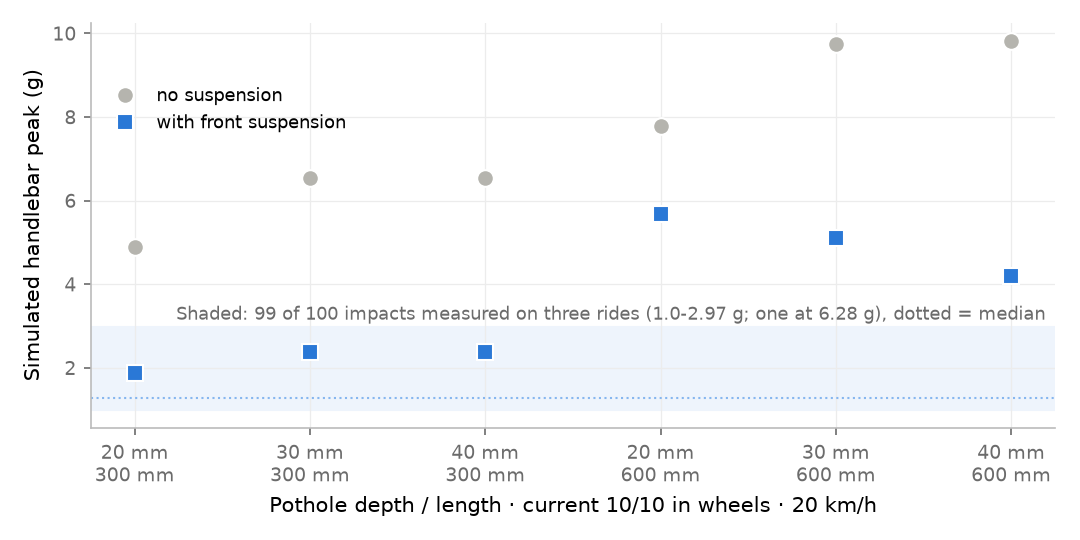
\includegraphics[width=\linewidth]{sim/consistency.png}
\caption{Consistency check: simulated handlebar peaks for the current 10/10 configuration at 20 km/h, with and without front suspension, against the range of 99 of the 100 impacts measured on the three rides (shaded; dotted line: median). Pothole depths on the route were not measured, so this is a consistency check, not a validation.}\label{fig:consistency}
\end{figure}

\subsection{Limitations of the models}\label{limitations-of-the-models}

\begin{itemize}
\tightlist
\item
  \textbf{Planar:} no steering, handlebar twist, roll or sideways falls. Loss of steering
  control, which a front-wheel impact can also cause, is not represented.
\item
  \textbf{Assumed vehicle:} mass, inertias, wheelbase, tyre stiffness, fork and the rear wheel
  size are not published by Voi.
\item
  \textbf{Simple rider:} one rigid body with a fixed spring; no active balance or reaction.
\item
  \textbf{Idealised potholes:} rectangular, or with smooth sloped edges; real potholes are
  irregular.
\item
  \textbf{Potholes only:} other obstacles were not part of the main study. An exploratory
  extension to raised bumps (Appendix~\ref{app:bumps}) found the same benefit of a larger
  front wheel without suspension, but with the front spring the few modelled bump falls
  started at the rigid rear wheel, so the front-wheel result may not hold for every type of
  obstacle.
\item
  \textbf{Analyst-defined falls} and a 10 mm depth resolution.
\item
  \textbf{Not validated} against physical tests; the consistency check is only a partial pass.
\end{itemize}

Within these limits, the models consistently show that the front wheel determines whether
the scooter pitches over, and that enlarging the front wheel alone gives the same benefit
in the model as enlarging both wheels.

% Discussion and conclusion (to be written after the Oxford Voiager 5 front tyre size is known; see DOCUMENTATION.md 12).
\section{Discussion}\label{sec:discussion}

[To be written.]

\section{Conclusion}\label{sec:conclusion}

[To be written.]

% Back-matter statements. [DOI to be added] placeholders must be filled in before
% submission; nothing has been deposited yet (2026-10-08).

\section*{Ethics}
\addcontentsline{toc}{section}{Ethics}

All recordings are of the author's own rides on rental e-scooters hired through the
operator's app within the official trial, ridden legally on public roads. The phone was
mounted on the handlebar before each ride and not handled while riding. No data about
other people were collected. A study recording other riders would need university
ethics approval and GDPR-compliant handling.

\section*{Data and code availability}
\addcontentsline{toc}{section}{Data and code availability}

\textbf{In this paper.} Every impact is listed in Table~\ref{tab:Aimpacts} (time, peak
acceleration, speed, road, spot), and every spot in Table~\ref{tab:C1}. The model results
behind each figure are summarised in Appendices~D and~\ref{app:model}.

\textbf{To be deposited} [DOI to be added]:
\begin{itemize}
\item \emph{Code:} the analysis and simulation scripts, which regenerate every figure and
  table from the data below.
\item \emph{Impact data:} the impact list with spot coordinates, the per-spot table and the
  FixMyStreet comparison, with the first and last 200 m of each route removed.
\item \emph{Model outputs:} all simulation results (one row per run) for the main sweep,
  sensitivity analysis, ratio study, soft-edge, bump and consistency experiments, and the
  geometry model sweep.
\item \emph{Recording quality:} the per-window features and labels used for walking
  detection and the data-quality summary.
\end{itemize}

\textbf{Not shared publicly.} The raw Sensor Logger recordings include the full GPS track,
including the start and end of each ride, and are therefore withheld for the author's
privacy. A version with the route ends removed is available from the author on request.

\textbf{Third-party data.} FixMyStreet reports (mySociety) and OpenStreetMap map data
(\copyright{} OpenStreetMap contributors) are subject to their providers' terms; the
deposit gives the query used and the download date instead of redistributing them where
those terms require it.


\printbibliography[heading=bibintoc]

\clearpage
\appendix
\appendixnumbering
% Guide to the appendices, placed before Appendix A.
\section*{Appendices at a glance}
\addcontentsline{toc}{section}{Appendices at a glance}

The appendices give the detail behind the main text. Each can be read on its own.

\begin{table}[h]
\centering\small\renewcommand{\arraystretch}{1.35}
\begin{tabular}{@{}l>{\raggedright\arraybackslash}p{38mm}>{\raggedright\arraybackslash}p{82mm}r@{}}
\toprule
 & Appendix & What it contains & Page \\
\midrule
\ref{individual-recordings} & Individual recordings
  & Each ride separately: summary tables, acceleration trace, severity, speed, impact and
    FixMyStreet maps; FixMyStreet comparison with reports of any date; list of all 100 impacts
  & \pageref{individual-recordings} \\
\ref{recording-quality-and-walking-detection} & Recording quality and walking detection
  & How reliable the Sensor Logger data are (sampling, noise, GPS), and how walking was told
    apart from riding, checked against the rider's references
  & \pageref{recording-quality-and-walking-detection} \\
\ref{visual-check-of-spots-in-street-level-imagery} & Visual check of spots
  & Method for checking impact spots in street-level imagery; every spot with links and QR
    codes (results pending)
  & \pageref{visual-check-of-spots-in-street-level-imagery} \\
\ref{app:bumps} & Road bumps
  & Exploratory, unvalidated extension of the model from potholes to raised bumps
  & \pageref{app:bumps} \\
\ref{app:model} & Further model results
  & Geometry model, full simulation sweeps, front/rear ratio study, soft pothole edges,
    fall thresholds without suspension and the sensitivity analysis
  & \pageref{app:model} \\
\bottomrule
\end{tabular}
\end{table}
\clearpage

% Converted from appendix_recordings.md by scripts/md_to_latex.py; edit this file.
% DRAFT v0.1 (2026-10-08). Appendices for Part A: individual recordings (A), recording
% quality and walking detection (B), visual check of spots (C).
% Numbers from outputs/recordings/<rec>/ (impact_stats.json, impacts_by_road.csv,
% fms_match_rates.csv), outputs/sensor_validity/ and outputs/combined/; figures copied to
% paper/figures/appendix/ by scripts/paper_part_a.py. Full methods: SENSOR_VALIDITY.md,
% SPOT_CHECK.md.

\section{Individual recordings}\label{individual-recordings}

The main text reports the three rides together. This appendix gives each ride on its
own. Hotspots here are numbered separately within each ride (impacts within 30 m of
each other in that ride); the spots P1--P33 of the main text are formed from the pooled
impacts and are numbered differently. Rates per km are left blank (--) where less than
0.2 km was ridden on a road.

% outputs/recordings/<rec>/impact_stats.json

\begin{longtable}[]{@{}
  >{\raggedright\arraybackslash}p{(\linewidth - 6\tabcolsep) * \real{0.2500}}
  >{\raggedright\arraybackslash}p{(\linewidth - 6\tabcolsep) * \real{0.2500}}
  >{\raggedright\arraybackslash}p{(\linewidth - 6\tabcolsep) * \real{0.2500}}
  >{\raggedright\arraybackslash}p{(\linewidth - 6\tabcolsep) * \real{0.2500}}@{}}
\caption{Impacts per ride.}\label{tab:A1}\tabularnewline
\toprule\noalign{}
\begin{minipage}[b]{\linewidth}\raggedright
\end{minipage} & \begin{minipage}[b]{\linewidth}\raggedright
Ride 1
\end{minipage} & \begin{minipage}[b]{\linewidth}\raggedright
Ride 2
\end{minipage} & \begin{minipage}[b]{\linewidth}\raggedright
Ride 3
\end{minipage} \\
\midrule\noalign{}
\endfirsthead
\toprule\noalign{}
\begin{minipage}[b]{\linewidth}\raggedright
\end{minipage} & \begin{minipage}[b]{\linewidth}\raggedright
Ride 1
\end{minipage} & \begin{minipage}[b]{\linewidth}\raggedright
Ride 2
\end{minipage} & \begin{minipage}[b]{\linewidth}\raggedright
Ride 3
\end{minipage} \\
\midrule\noalign{}
\endhead
\bottomrule\noalign{}
\endlastfoot
Date, start (local) & 3 Oct, 18:30 & 7 Oct, 10:37 & 7 Oct, 13:38 \\
Vehicle (Voiager 5) & SZ22 & UPAR & BTLZ \\
Distance ridden & 2.89 km & 1.48 km & 1.71 km \\
Riding time; mean riding speed & 9.6 min; 18.1 km/h & 5.9 min; 15.1 km/h & 6.3 min; 16.4 km/h \\
Impacts (per km; metres between) & 40 (13.8; 72 m) & 39 (26.4; 38 m) & 21 (12.3; 81 m) \\
Median peak (interquartile range) & 1.19 g (1.13--1.35) & 1.34 g (1.19--1.77) & 1.67 g (1.13--1.85) \\
Maximum & 2.80 g & 2.87 g & 6.28 g \\
≥ 1.5 g; ≥ 2.0 g & 6; 4 & 15; 3 & 11; 5 \\
Marked wobble; also ≥ 1.5 g & 13; 3 & 11; 5 & 8; 4 \\
Speed vs peak, Spearman ρ (p) & 0.03 (0.88) & −0.63 (\textless{} 0.001) & −0.68 (0.001) \\
Hotspots within the ride (2+ impacts) & 11 & 6 & 3 \\
\end{longtable}

% outputs/recordings/<rec>/impacts_by_road.csv

\begin{longtable}[]{@{}
  >{\raggedright\arraybackslash}p{(\linewidth - 6\tabcolsep) * \real{0.2500}}
  >{\raggedright\arraybackslash}p{(\linewidth - 6\tabcolsep) * \real{0.2500}}
  >{\raggedright\arraybackslash}p{(\linewidth - 6\tabcolsep) * \real{0.2500}}
  >{\raggedright\arraybackslash}p{(\linewidth - 6\tabcolsep) * \real{0.2500}}@{}}
\caption{Impacts per km by road and ride (km ridden in brackets).}\label{tab:A2}\tabularnewline
\toprule\noalign{}
\begin{minipage}[b]{\linewidth}\raggedright
Road
\end{minipage} & \begin{minipage}[b]{\linewidth}\raggedright
Ride 1
\end{minipage} & \begin{minipage}[b]{\linewidth}\raggedright
Ride 2
\end{minipage} & \begin{minipage}[b]{\linewidth}\raggedright
Ride 3
\end{minipage} \\
\midrule\noalign{}
\endfirsthead
\toprule\noalign{}
\begin{minipage}[b]{\linewidth}\raggedright
Road
\end{minipage} & \begin{minipage}[b]{\linewidth}\raggedright
Ride 1
\end{minipage} & \begin{minipage}[b]{\linewidth}\raggedright
Ride 2
\end{minipage} & \begin{minipage}[b]{\linewidth}\raggedright
Ride 3
\end{minipage} \\
\midrule\noalign{}
\endhead
\bottomrule\noalign{}
\endlastfoot
Marston Road & 11.6 (0.95 km) & 15.8 (0.82 km) & 9.3 (0.75 km) \\
Morrell Avenue & 12.2 (0.98 km) & -- (0.04 km, 3 impacts) & -- (0.03 km, 0 impacts) \\
Old Road & 8.2 (0.24 km) & not ridden & not ridden \\
Headington Road & not ridden & -- (0.02 km, 1 impact) & not ridden \\
Other roads & 21.0 (0.72 km) & 36.7 (0.60 km) & 15.1 (0.93 km) \\
\end{longtable}

% outputs/recordings/<rec>/fms_match_rates.csv

\begin{longtable}[]{@{}
  >{\raggedright\arraybackslash}p{(\linewidth - 6\tabcolsep) * \real{0.2500}}
  >{\raggedright\arraybackslash}p{(\linewidth - 6\tabcolsep) * \real{0.2500}}
  >{\raggedright\arraybackslash}p{(\linewidth - 6\tabcolsep) * \real{0.2500}}
  >{\raggedright\arraybackslash}p{(\linewidth - 6\tabcolsep) * \real{0.2500}}@{}}
\caption{Impacts with a road-surface FixMyStreet report made in the 365 days before the ride within 15, 25 and 50 m, against the same share for all points on the ridden route (baseline).}\label{tab:A3}\tabularnewline
\toprule\noalign{}
\begin{minipage}[b]{\linewidth}\raggedright
Radius
\end{minipage} & \begin{minipage}[b]{\linewidth}\raggedright
Ride 1: impacts / baseline
\end{minipage} & \begin{minipage}[b]{\linewidth}\raggedright
Ride 2: impacts / baseline
\end{minipage} & \begin{minipage}[b]{\linewidth}\raggedright
Ride 3: impacts / baseline
\end{minipage} \\
\midrule\noalign{}
\endfirsthead
\toprule\noalign{}
\begin{minipage}[b]{\linewidth}\raggedright
Radius
\end{minipage} & \begin{minipage}[b]{\linewidth}\raggedright
Ride 1: impacts / baseline
\end{minipage} & \begin{minipage}[b]{\linewidth}\raggedright
Ride 2: impacts / baseline
\end{minipage} & \begin{minipage}[b]{\linewidth}\raggedright
Ride 3: impacts / baseline
\end{minipage} \\
\midrule\noalign{}
\endhead
\bottomrule\noalign{}
\endlastfoot
15 m & 5.0\% / 7.7\% & 15.4\% / 20.7\% & 28.6\% / 19.4\% \\
25 m & 5.0\% / 14.3\% & 30.8\% / 32.7\% & 42.9\% / 34.3\% \\
50 m & 17.5\% / 28.2\% & 69.2\% / 53.1\% & 66.7\% / 54.0\% \\
\end{longtable}

% outputs/recordings/<rec>/fms_match_rates.csv (any-date columns)
\begin{table}[htbp]
\centering\small
\caption{As Table~\ref{tab:A3}, but with FixMyStreet road-surface reports of any date since 2009. Most route points lie near some report, so these shares measure report density rather than reporting of the impacts; this is why the main comparison uses only the 365 days before each ride.}\label{tab:A3any}
\begin{tabular}{@{}lrrr@{}}
\toprule
Radius & Ride 1: impacts / baseline & Ride 2: impacts / baseline & Ride 3: impacts / baseline \\
\midrule
15 m & 42.5\% / 52.3\% & 84.6\% / 75.0\% & 81.0\% / 74.2\% \\
25 m & 62.5\% / 70.3\% & 87.2\% / 84.9\% & 100.0\% / 87.0\% \\
50 m & 72.5\% / 85.9\% & 89.7\% / 93.8\% & 100.0\% / 94.1\% \\
\bottomrule
\end{tabular}
\end{table}

Each ride was compared with reports downloaded for its own route's area (ride 1 on
3 October 2026, rides 2 and 3 on 8 October 2026). In ride 1, none of the six impacts of
1.5 g or more and one of its eleven hotspots had a recent report within 25 m.

\textbf{Notes per ride.}

\begin{itemize}
\tightlist
\item
  \textbf{Ride 1.} One hotspot (near 51.7522, −1.2377; spot P12 in the main text) was hit on
  three separate passes, up to 2.68 g. It lies 6 m from a pothole reported in January
  2026 and marked ``fixed''. The two strongest impacts (2.80 g and 2.68 g) came at low
  speed just after a stop.
\item
  \textbf{Ride 2.} Thirteen impacts followed each other every 0.6--1.2 s at about 8 km/h over
  roughly 20 m (spot P3). The ride ended at 10:46 (Voi rental end); the walk that
  followed is excluded by the speed rule (Appendix B).
\item
  \textbf{Ride 3.} The strongest impact of all rides, 6.28 g at 8.1 km/h, was followed by four
  more impacts of 1.8--3.0 g within about 4 s (spot P4).
\end{itemize}

\FloatBarrier
\subsection{Ride 1 figures}

\begin{figure}
\centering
{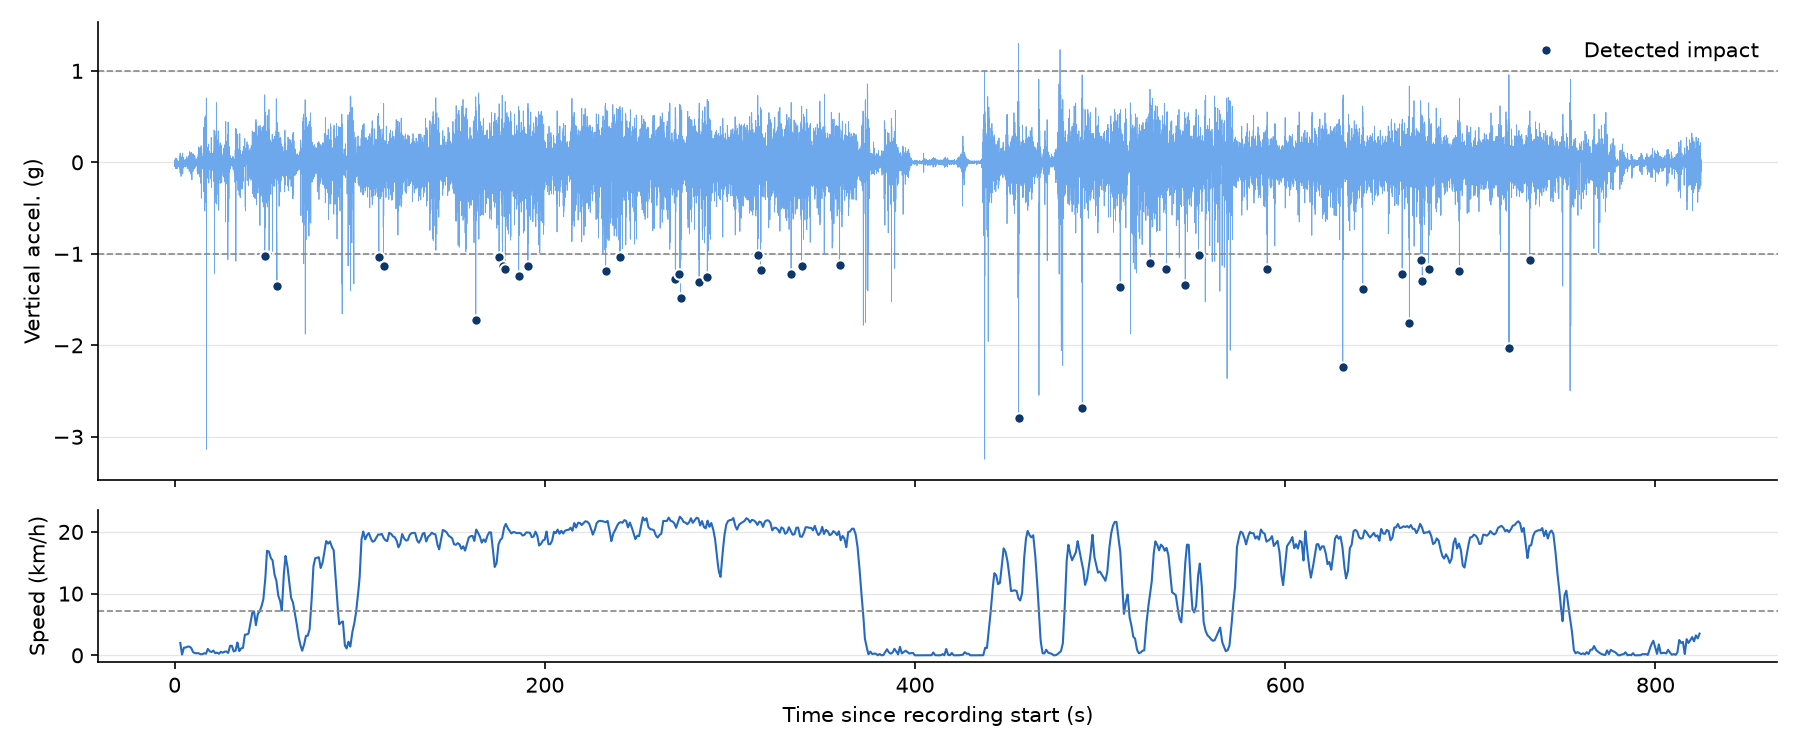
\includegraphics[width=\linewidth]{appendix/2026-10-03_1830_rec01_impact_trace.png}}
\caption{Ride 1: vertical acceleration (top) and GPS speed (bottom) over the recording, with detected impacts. Dashed lines: ±1 g threshold and 7 km/h speed rule.}\label{fig:A1}
\end{figure}

\begin{figure}
\centering
{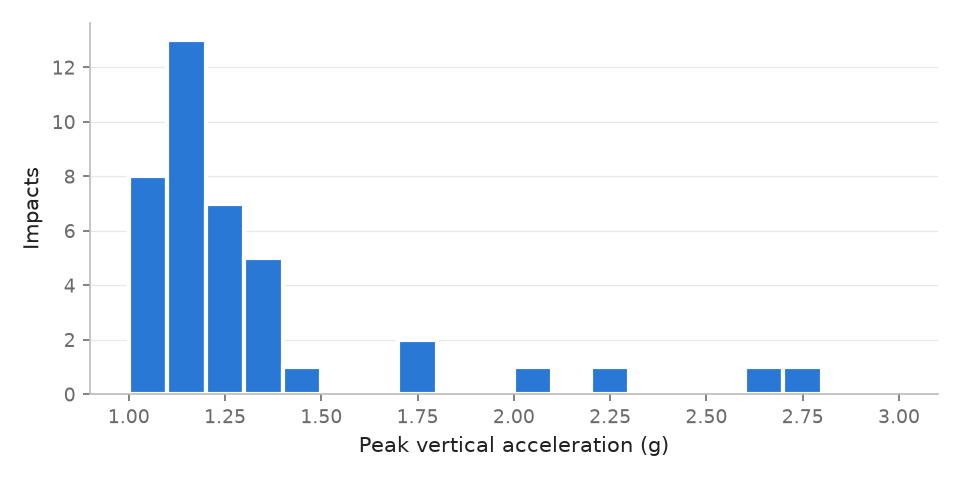
\includegraphics[width=\linewidth]{appendix/2026-10-03_1830_rec01_fig_severity_hist.png}}
\caption{Ride 1: peak vertical acceleration of the 40 impacts.}\label{fig:A2}
\end{figure}

\begin{figure}
\centering
{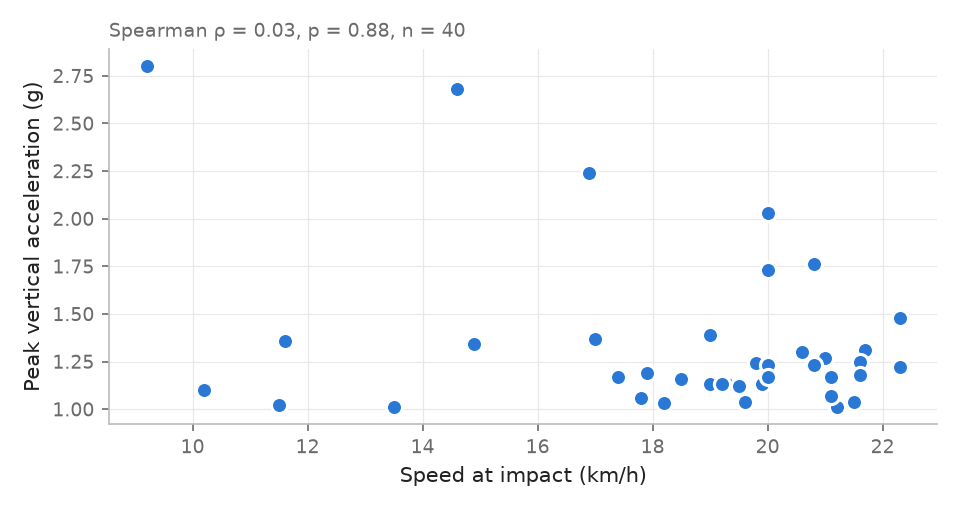
\includegraphics[width=\linewidth]{appendix/2026-10-03_1830_rec01_fig_speed_vs_severity.png}}
\caption{Ride 1: GPS speed against peak vertical acceleration for each impact. One ride; no trend is claimed.}\label{fig:A3}
\end{figure}

\begin{figure}
\centering
{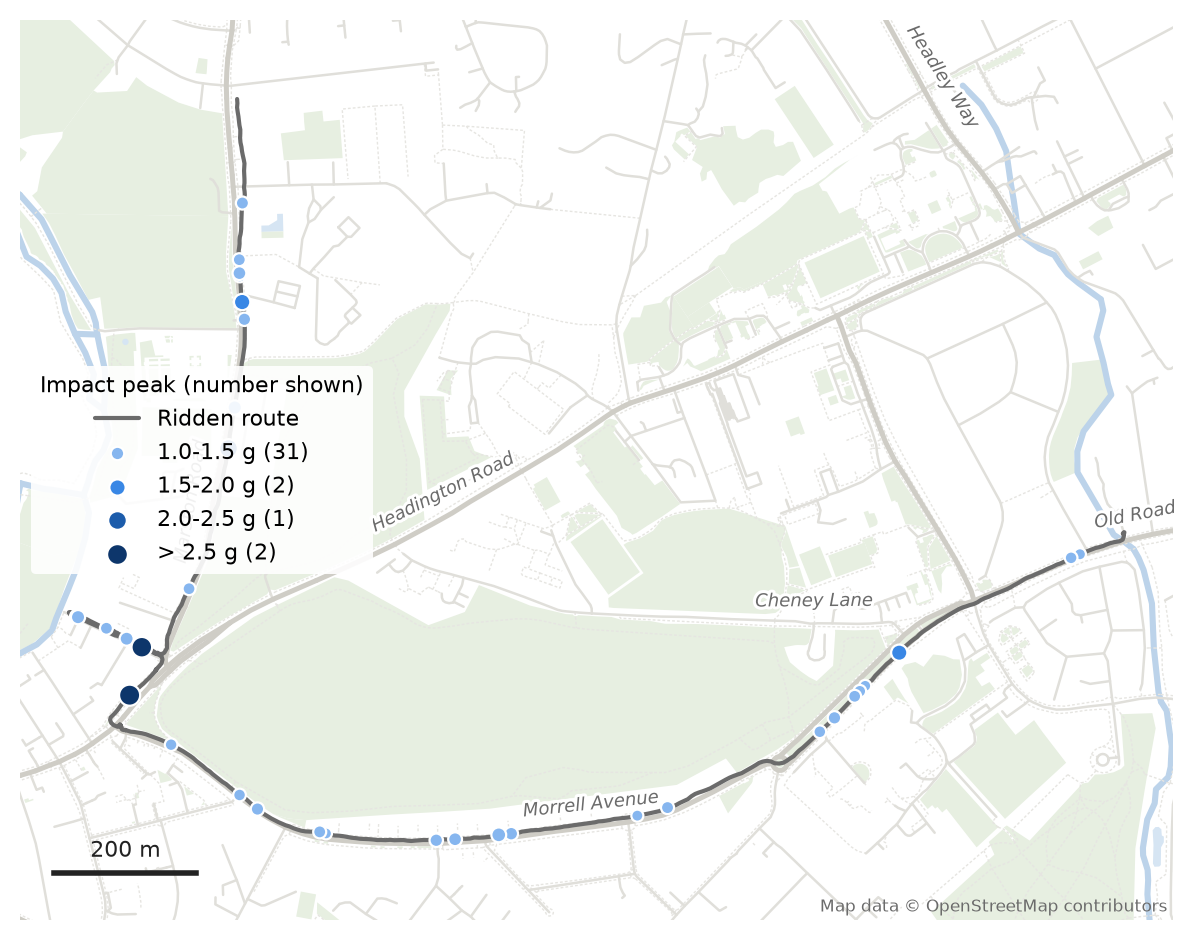
\includegraphics[width=\linewidth]{appendix/2026-10-03_1830_rec01_impact_map.png}}
\caption{Ride 1: impacts on the ridden route, coloured by severity band (bands are analyst choices). Route ends (200 m) and impacts or reports near them are not drawn, for privacy; such impacts are still counted in Table~\ref{tab:A1}. Map data \copyright{} OpenStreetMap contributors.}\label{fig:A4}
\end{figure}

\begin{figure}
\centering
{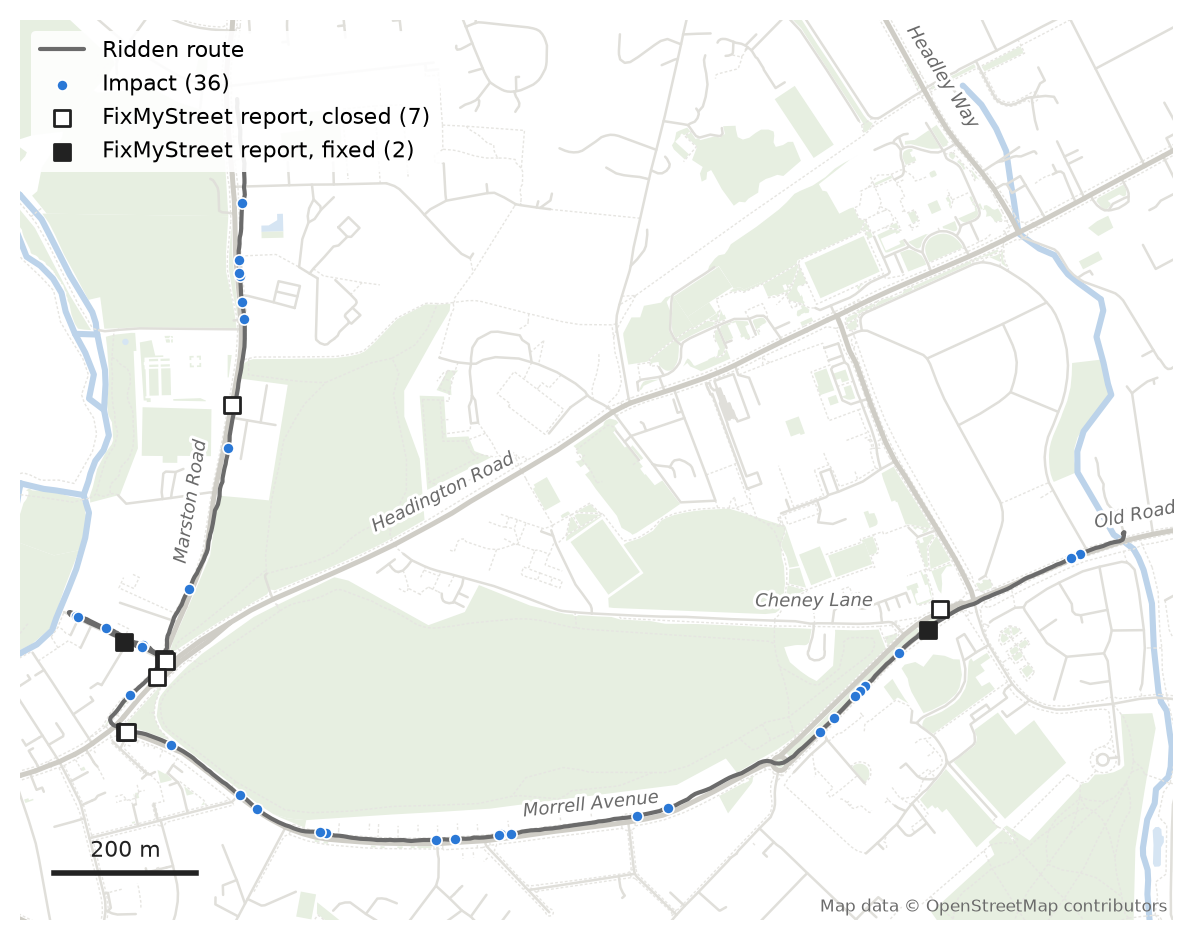
\includegraphics[width=\linewidth]{appendix/2026-10-03_1830_rec01_fms_map.png}}
\caption{Ride 1: impacts and FixMyStreet road-surface reports made in the 365 days before the ride (hollow: closed; filled: marked fixed). A report near an impact does not show that it refers to the same defect. Route ends (200 m) and impacts or reports near them are not drawn, for privacy; such impacts are still counted in Table~\ref{tab:A1}. Map data \copyright{} OpenStreetMap contributors.}\label{fig:A5}
\end{figure}

\FloatBarrier
\subsection{Ride 2 figures}

\begin{figure}
\centering
{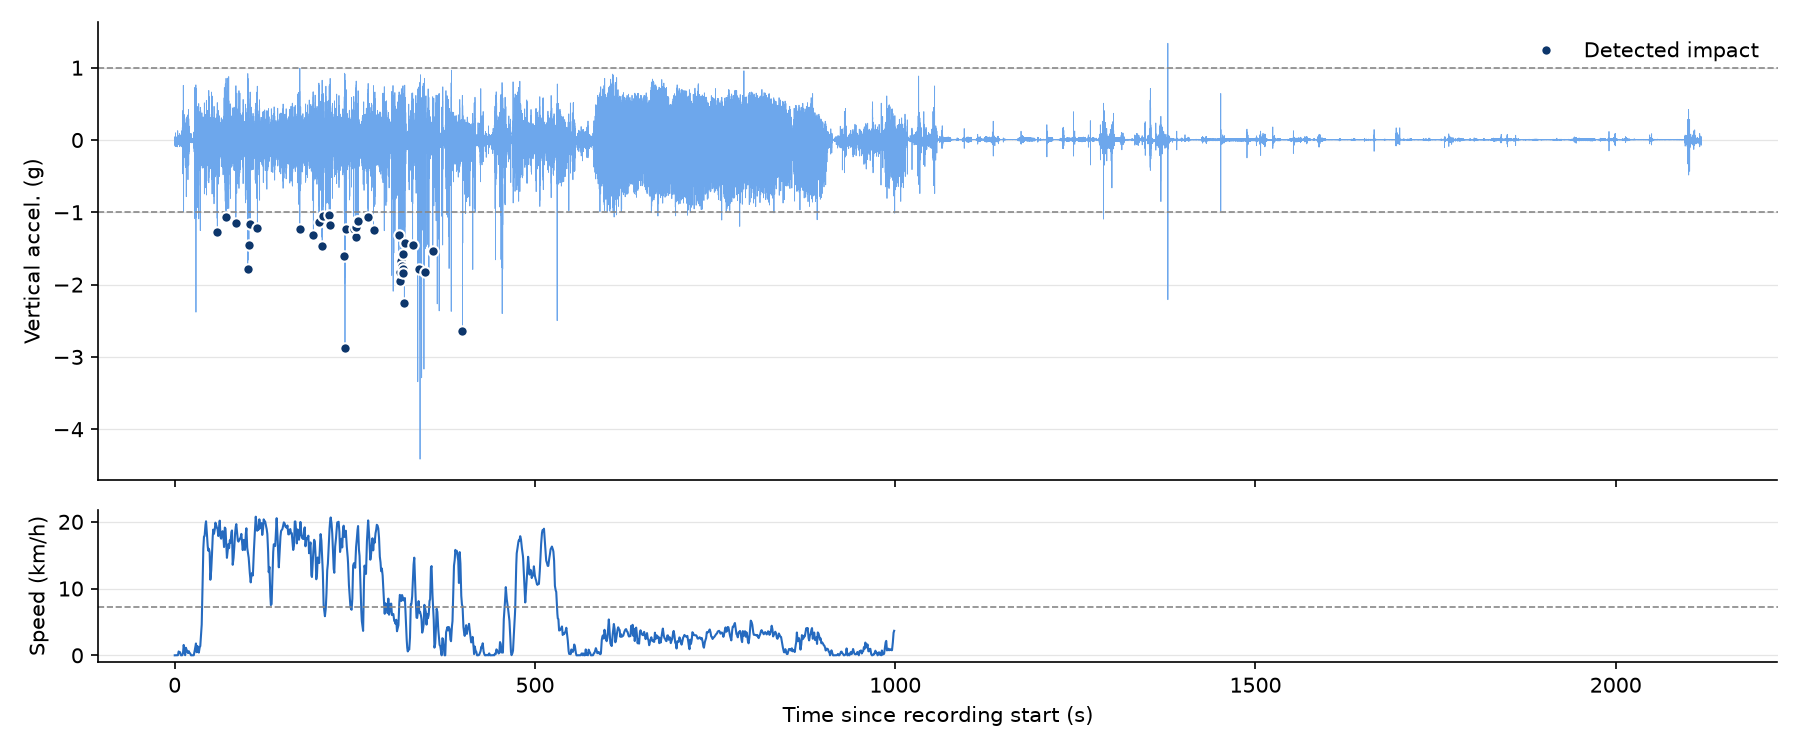
\includegraphics[width=\linewidth]{appendix/2026-10-07_1037_rec02_impact_trace.png}}
\caption{Ride 2: vertical acceleration (top) and GPS speed (bottom) over the recording, with detected impacts. The walk (about 580--900 s) and the phone at rest afterwards produce no impacts because of the speed rule.}\label{fig:A6}
\end{figure}

\begin{figure}
\centering
{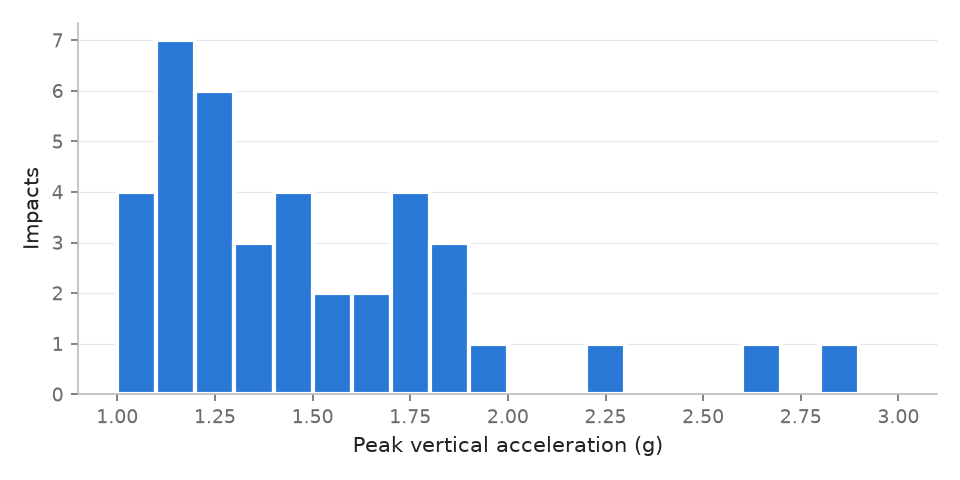
\includegraphics[width=\linewidth]{appendix/2026-10-07_1037_rec02_fig_severity_hist.png}}
\caption{Ride 2: peak vertical acceleration of the 39 impacts.}\label{fig:A7}
\end{figure}

\begin{figure}
\centering
{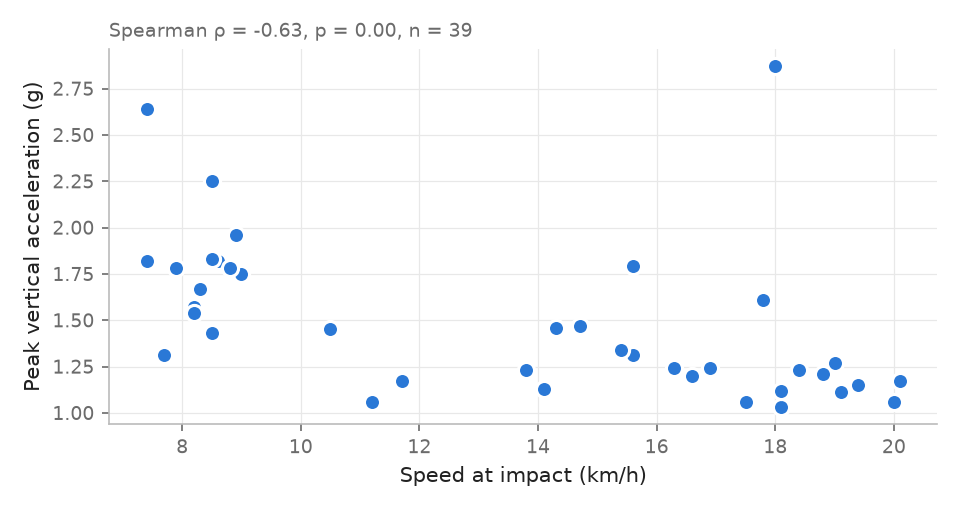
\includegraphics[width=\linewidth]{appendix/2026-10-07_1037_rec02_fig_speed_vs_severity.png}}
\caption{Ride 2: GPS speed against peak vertical acceleration for each impact. One ride; no trend is claimed.}\label{fig:A8}
\end{figure}

\begin{figure}
\centering
{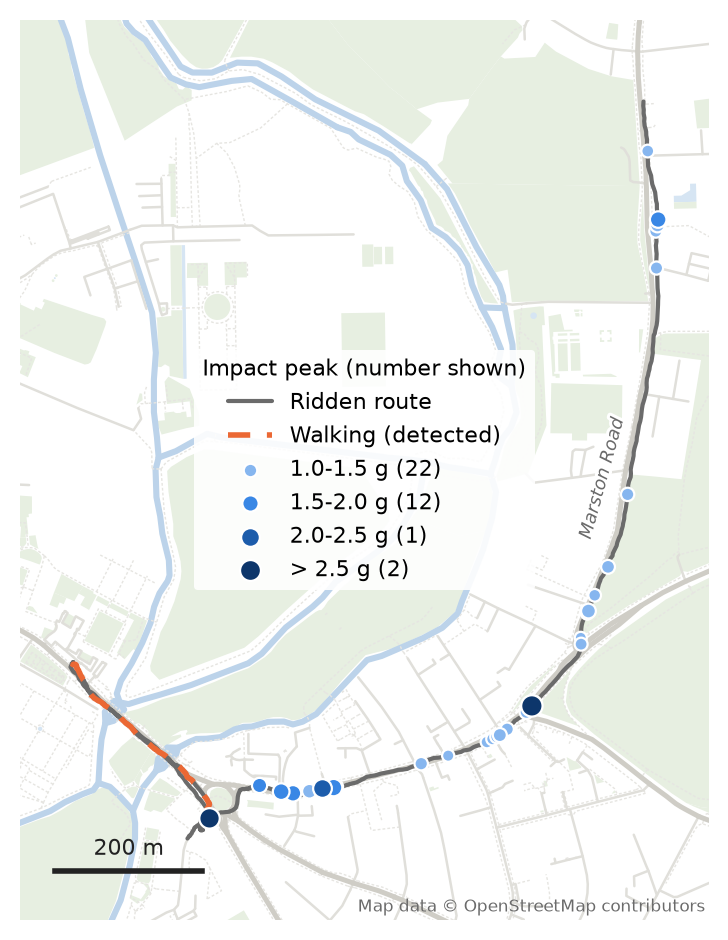
\includegraphics[width=\linewidth]{appendix/2026-10-07_1037_rec02_impact_map.png}}
\caption{Ride 2: impacts on the ridden route, coloured by severity band (bands are analyst choices). The dashed orange line is the walk detected in Appendix~B (not ridden; no impacts are counted there). Route ends (200 m) and impacts or reports near them are not drawn, for privacy; such impacts are still counted in Table~\ref{tab:A1}. Map data \copyright{} OpenStreetMap contributors.}\label{fig:A9}
\end{figure}

\begin{figure}
\centering
{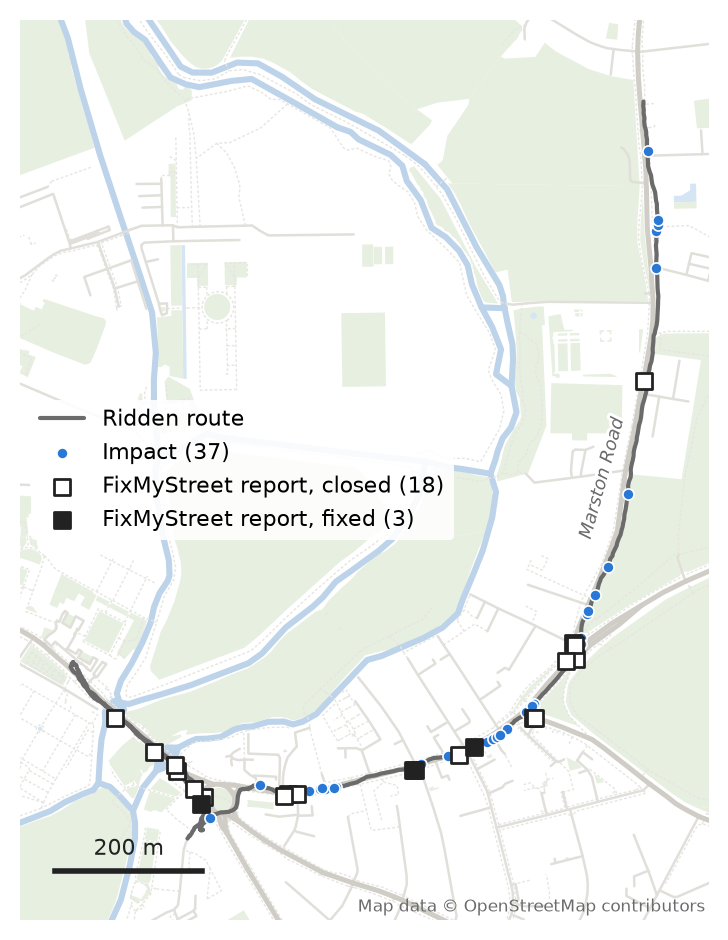
\includegraphics[width=\linewidth]{appendix/2026-10-07_1037_rec02_fms_map.png}}
\caption{Ride 2: impacts and FixMyStreet road-surface reports made in the 365 days before the ride (hollow: closed; filled: marked fixed). A report near an impact does not show that it refers to the same defect. Route ends (200 m) and impacts or reports near them are not drawn, for privacy; such impacts are still counted in Table~\ref{tab:A1}. Map data \copyright{} OpenStreetMap contributors.}\label{fig:A10}
\end{figure}

\FloatBarrier
\subsection{Ride 3 figures}

\begin{figure}
\centering
{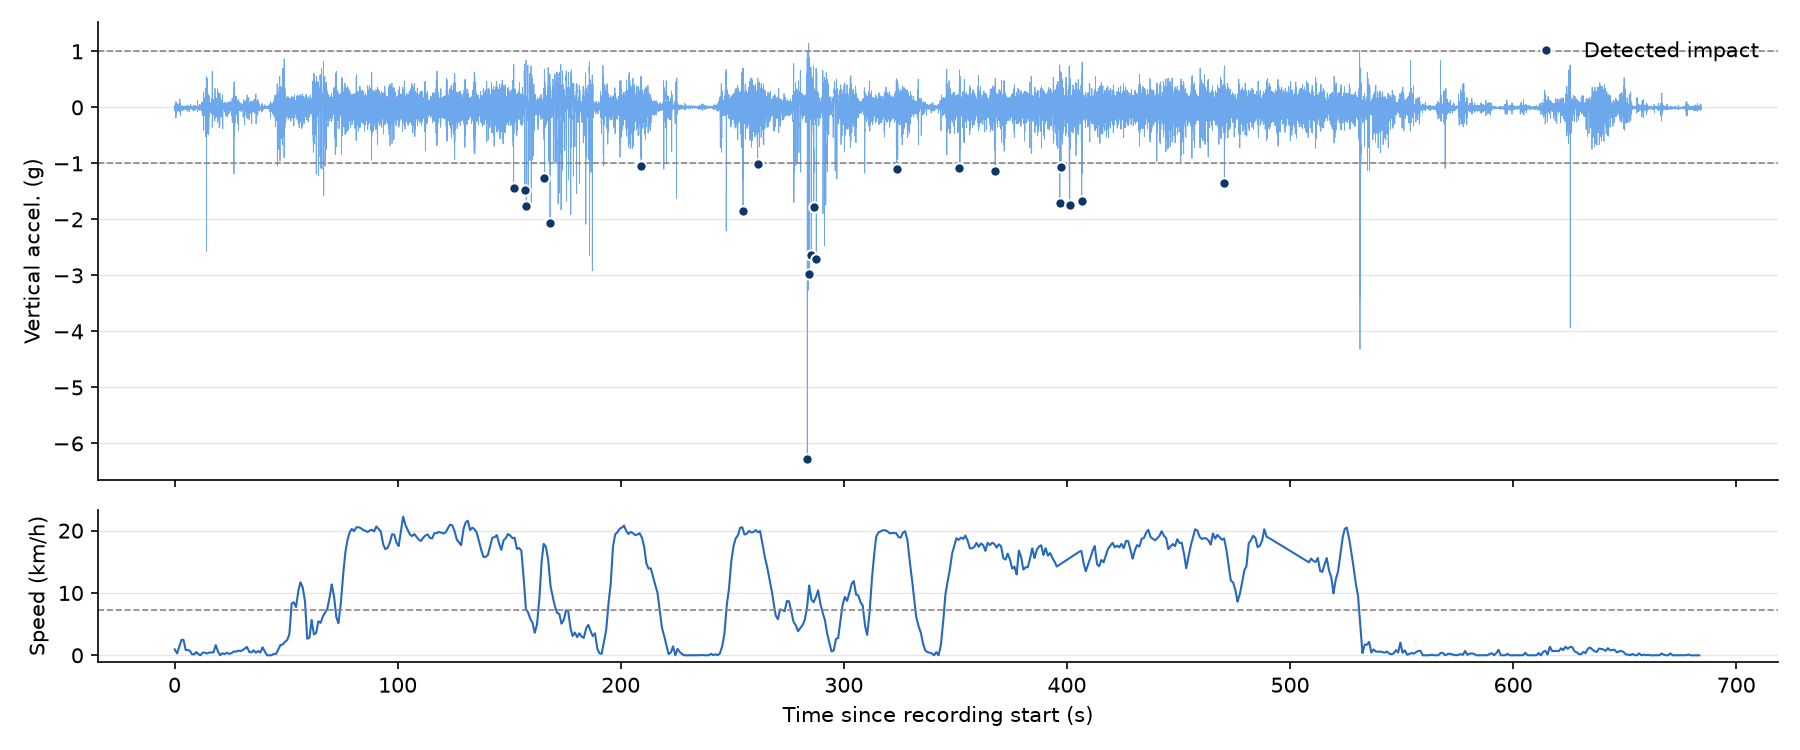
\includegraphics[width=\linewidth]{appendix/2026-10-07_1338_rec03_impact_trace.png}}
\caption{Ride 3: vertical acceleration (top) and GPS speed (bottom) over the recording, with detected impacts.}\label{fig:A11}
\end{figure}

\begin{figure}
\centering
{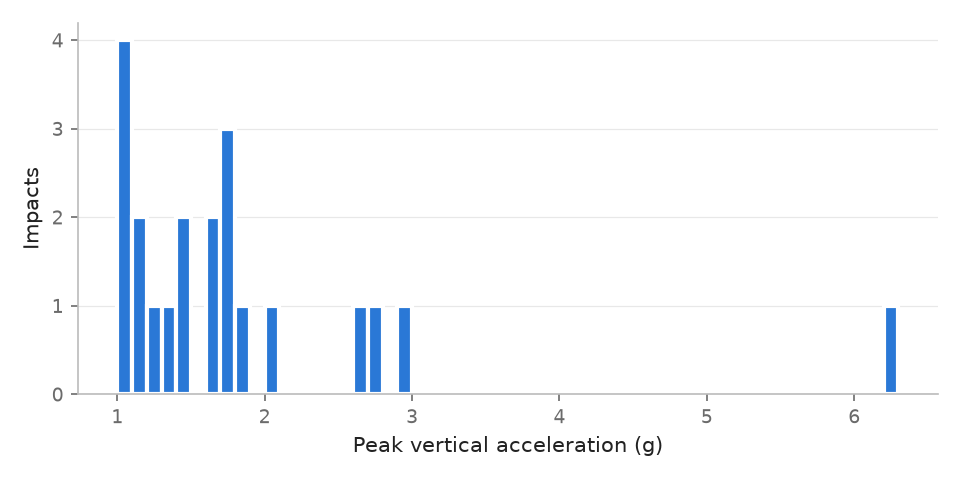
\includegraphics[width=\linewidth]{appendix/2026-10-07_1338_rec03_fig_severity_hist.png}}
\caption{Ride 3: peak vertical acceleration of the 21 impacts.}\label{fig:A12}
\end{figure}

\begin{figure}
\centering
{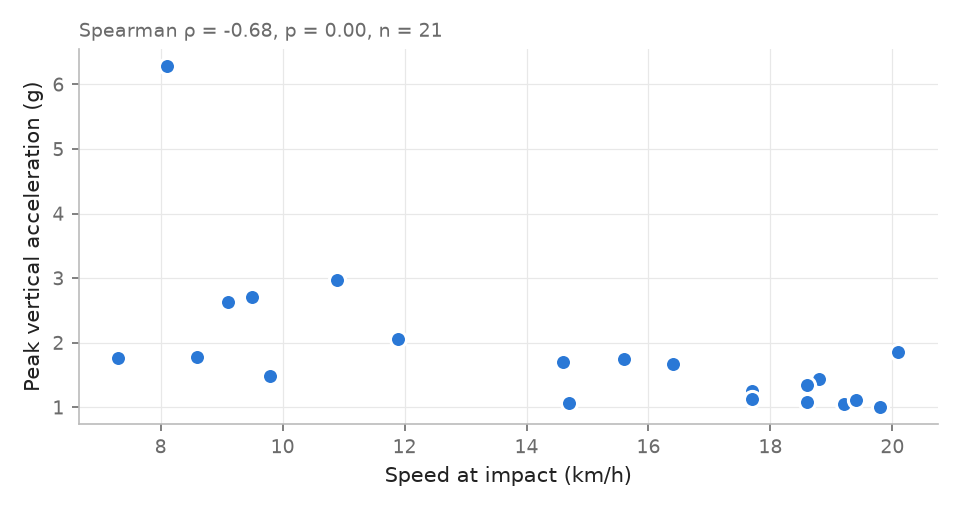
\includegraphics[width=\linewidth]{appendix/2026-10-07_1338_rec03_fig_speed_vs_severity.png}}
\caption{Ride 3: GPS speed against peak vertical acceleration for each impact. One ride; no trend is claimed.}\label{fig:A13}
\end{figure}

\begin{figure}
\centering
{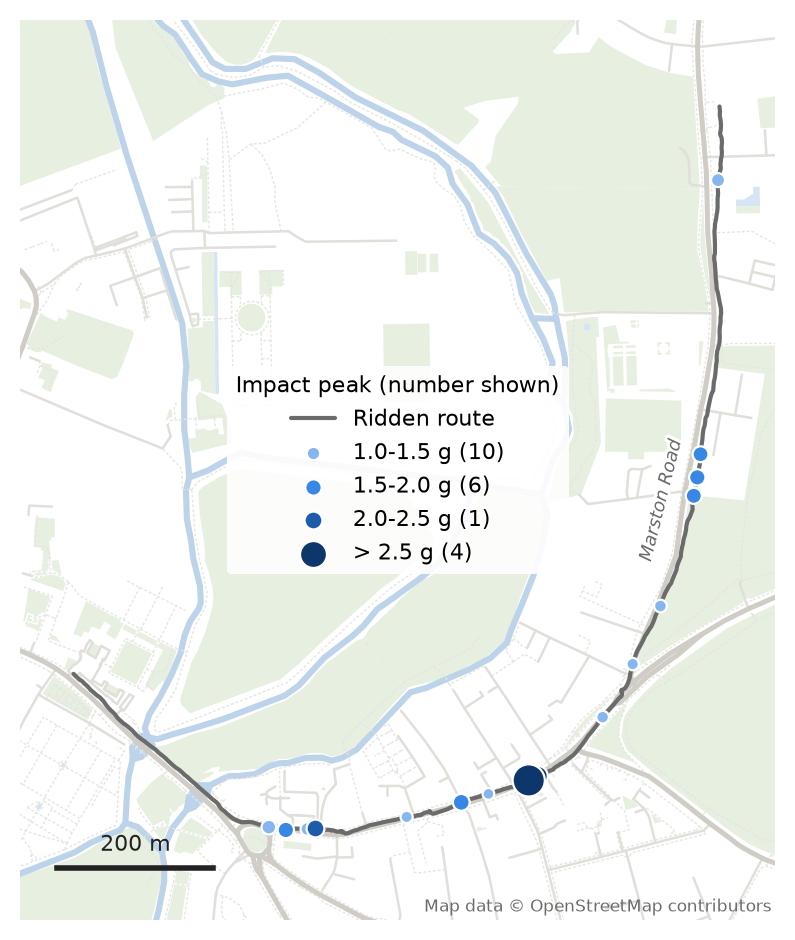
\includegraphics[width=\linewidth]{appendix/2026-10-07_1338_rec03_impact_map.png}}
\caption{Ride 3: impacts on the ridden route, coloured by severity band (bands are analyst choices). Route ends (200 m) and impacts or reports near them are not drawn, for privacy; such impacts are still counted in Table~\ref{tab:A1}. Map data \copyright{} OpenStreetMap contributors.}\label{fig:A14}
\end{figure}

\begin{figure}
\centering
{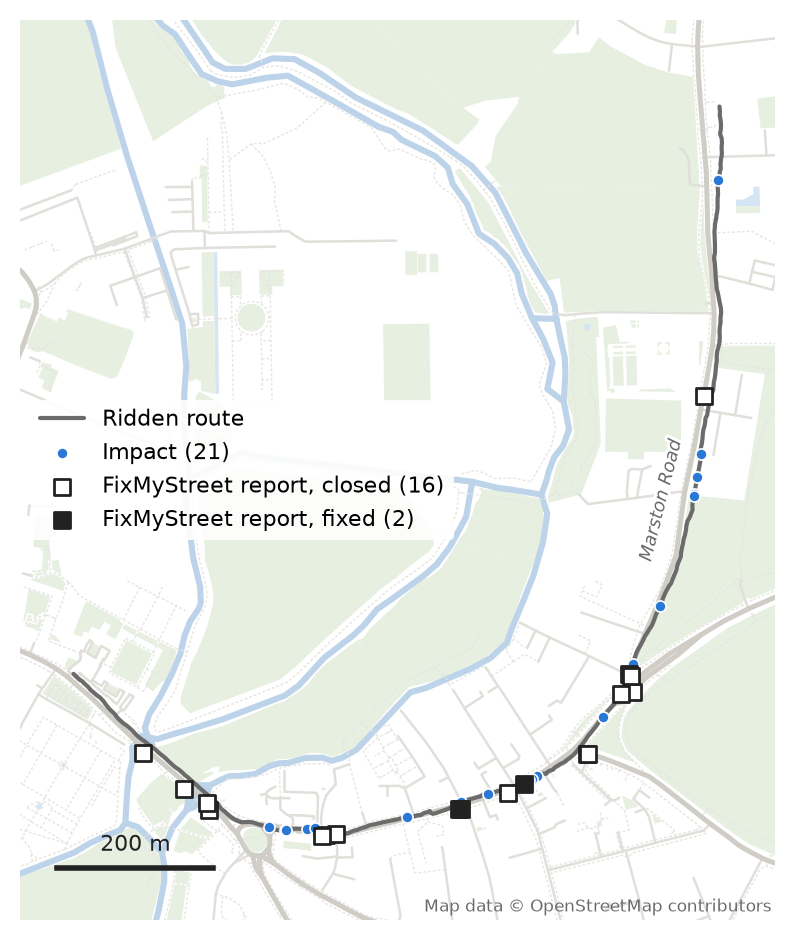
\includegraphics[width=\linewidth]{appendix/2026-10-07_1338_rec03_fms_map.png}}
\caption{Ride 3: impacts and FixMyStreet road-surface reports made in the 365 days before the ride (hollow: closed; filled: marked fixed). A report near an impact does not show that it refers to the same defect. Route ends (200 m) and impacts or reports near them are not drawn, for privacy; such impacts are still counted in Table~\ref{tab:A1}. Map data \copyright{} OpenStreetMap contributors.}\label{fig:A15}
\end{figure}

\FloatBarrier
\subsection{All impacts}
% outputs/combined/impacts_all.csv, outputs/combined/spot_links.csv
\begingroup\small
\begin{longtable}{@{}rrlrrllll@{}}
\caption{All 100 detected impacts. Time is local (Europe/London); speed is GPS speed at the impact; wobble = gyroscope ratio $\geq$ 1.5 after vs before (an analyst choice); report = a FixMyStreet road-surface report made in the 365 days before the ride within 25 m; spot = location in Table~\ref{tab:C1} (spots P9, P16, P30 and P31 lie in the trimmed route ends and have no location there). Coordinates are not listed, for privacy; the anonymised dataset is described under Data availability.}\label{tab:Aimpacts}\\
\toprule
Ride & \# & Time & Peak (g) & Speed (km/h) & Wobble & Road & Report $\leq$25 m & Spot \\
\midrule
\endfirsthead
\toprule
Ride & \# & Time & Peak (g) & Speed (km/h) & Wobble & Road & Report $\leq$25 m & Spot \\
\midrule
\endhead
\bottomrule
\endlastfoot
1 & 1 & 18:31:17 & 1.02 & 11.5 &  & Other roads &  & P16 \\
1 & 2 & 18:31:24 & 1.36 & 11.6 & yes & Other roads &  & P16 \\
1 & 3 & 18:32:19 & 1.04 & 19.6 & yes & Old Road &  & P20 \\
1 & 4 & 18:32:21 & 1.13 & 19.0 &  & Old Road &  & P20 \\
1 & 5 & 18:33:11 & 1.73 & 20.0 &  & Other roads &  & P22 \\
1 & 6 & 18:33:24 & 1.03 & 18.2 &  & Other roads &  & P14 \\
1 & 7 & 18:33:26 & 1.13 & 19.3 &  & Other roads &  & P14 \\
1 & 8 & 18:33:27 & 1.17 & 21.1 &  & Other roads &  & P14 \\
1 & 9 & 18:33:34 & 1.24 & 19.8 &  & Other roads &  & P18 \\
1 & 10 & 18:33:39 & 1.13 & 19.9 &  & Other roads &  & P18 \\
1 & 11 & 18:34:21 & 1.19 & 21.6 &  & Morrell Avenue &  & P25 \\
1 & 12 & 18:34:29 & 1.04 & 21.5 &  & Morrell Avenue &  & P33 \\
1 & 13 & 18:34:59 & 1.27 & 21.0 & yes & Morrell Avenue &  & P13 \\
1 & 14 & 18:35:01 & 1.22 & 22.3 & yes & Morrell Avenue &  & P13 \\
1 & 15 & 18:35:02 & 1.48 & 22.3 &  & Morrell Avenue &  & P13 \\
1 & 16 & 18:35:12 & 1.31 & 21.7 & yes & Morrell Avenue &  & P17 \\
1 & 17 & 18:35:16 & 1.25 & 21.6 &  & Morrell Avenue &  & P17 \\
1 & 18 & 18:35:44 & 1.01 & 21.2 & yes & Morrell Avenue &  & P19 \\
1 & 19 & 18:35:45 & 1.18 & 21.6 &  & Morrell Avenue &  & P19 \\
1 & 20 & 18:36:02 & 1.23 & 20.0 &  & Morrell Avenue &  & P24 \\
1 & 21 & 18:36:07 & 1.13 & 19.2 &  & Morrell Avenue &  & P28 \\
1 & 22 & 18:36:28 & 1.12 & 19.5 &  & Morrell Avenue &  & P29 \\
1 & 23 & 18:38:05 & 2.80 & 9.2 & yes & Other roads &  & P8 \\
1 & 24 & 18:38:39 & 2.68 & 14.6 &  & Other roads &  & P12 \\
1 & 25 & 18:38:59 & 1.37 & 17.0 &  & Other roads &  & P15 \\
1 & 26 & 18:39:16 & 1.10 & 10.2 &  & Other roads &  & P15 \\
1 & 27 & 18:39:24 & 1.17 & 17.4 & yes & Other roads &  & P26 \\
1 & 28 & 18:39:35 & 1.34 & 14.9 &  & Other roads & yes & P12 \\
1 & 29 & 18:39:42 & 1.01 & 13.5 &  & Other roads &  & P12 \\
1 & 30 & 18:40:19 & 1.16 & 18.5 & yes & Marston Road &  & P2 \\
1 & 31 & 18:41:00 & 2.24 & 16.9 &  & Marston Road &  & P1 \\
1 & 32 & 18:41:10 & 1.39 & 19.0 &  & Marston Road & yes & P23 \\
1 & 33 & 18:41:32 & 1.23 & 20.8 &  & Marston Road &  & P5 \\
1 & 34 & 18:41:36 & 1.76 & 20.8 & yes & Marston Road &  & P5 \\
1 & 35 & 18:41:42 & 1.07 & 21.1 & yes & Marston Road &  & P5 \\
1 & 36 & 18:41:43 & 1.30 & 20.6 &  & Marston Road &  & P5 \\
1 & 37 & 18:41:46 & 1.17 & 20.0 &  & Marston Road &  & P5 \\
1 & 38 & 18:42:03 & 1.19 & 17.9 & yes & Marston Road &  & P10 \\
1 & 39 & 18:42:29 & 2.03 & 20.0 & yes & Marston Road &  & P9 \\
1 & 40 & 18:42:41 & 1.06 & 17.8 &  & Marston Road &  & P30 \\
\midrule
2 & 1 & 10:38:05 & 1.27 & 19.0 &  & Marston Road &  & P9 \\
2 & 2 & 10:38:17 & 1.06 & 17.5 &  & Marston Road &  & P31 \\
2 & 3 & 10:38:31 & 1.15 & 19.4 & yes & Marston Road &  & P27 \\
2 & 4 & 10:38:47 & 1.79 & 15.6 & yes & Marston Road &  & P5 \\
2 & 5 & 10:38:49 & 1.46 & 14.3 &  & Marston Road &  & P5 \\
2 & 6 & 10:38:51 & 1.17 & 11.7 &  & Marston Road &  & P5 \\
2 & 7 & 10:39:01 & 1.21 & 18.8 &  & Marston Road &  & P5 \\
2 & 8 & 10:40:00 & 1.23 & 18.4 &  & Marston Road &  & P1 \\
2 & 9 & 10:40:18 & 1.31 & 15.6 & yes & Marston Road &  & P2 \\
2 & 10 & 10:40:27 & 1.13 & 14.1 &  & Marston Road &  & P2 \\
2 & 11 & 10:40:31 & 1.47 & 14.7 & yes & Marston Road &  & P2 \\
2 & 12 & 10:40:32 & 1.06 & 11.2 &  & Marston Road &  & P2 \\
2 & 13 & 10:40:40 & 1.03 & 18.1 & yes & Marston Road & yes & P7 \\
2 & 14 & 10:40:42 & 1.17 & 20.1 &  & Headington Road & yes & P7 \\
2 & 15 & 10:41:02 & 1.61 & 17.8 & yes & Morrell Avenue & yes & P11 \\
2 & 16 & 10:41:02 & 2.87 & 18.0 & yes & Morrell Avenue & yes & P11 \\
2 & 17 & 10:41:04 & 1.24 & 16.9 &  & Morrell Avenue & yes & P11 \\
2 & 18 & 10:41:15 & 1.23 & 13.8 &  & Other roads &  & P4 \\
2 & 19 & 10:41:17 & 1.34 & 15.4 & yes & Other roads &  & P4 \\
2 & 20 & 10:41:18 & 1.20 & 16.6 &  & Other roads &  & P4 \\
2 & 21 & 10:41:19 & 1.12 & 18.1 &  & Other roads &  & P4 \\
2 & 22 & 10:41:21 & 1.11 & 19.1 &  & Other roads & yes & P4 \\
2 & 23 & 10:41:34 & 1.06 & 20.0 &  & Other roads & yes & P6 \\
2 & 24 & 10:41:42 & 1.24 & 16.3 & yes & Other roads & yes & P6 \\
2 & 25 & 10:42:18 & 1.31 & 7.7 &  & Other roads &  & P3 \\
2 & 26 & 10:42:19 & 1.96 & 8.9 &  & Other roads &  & P3 \\
2 & 27 & 10:42:19 & 1.82 & 8.6 &  & Other roads &  & P3 \\
2 & 28 & 10:42:21 & 1.67 & 8.3 &  & Other roads &  & P3 \\
2 & 29 & 10:42:21 & 1.75 & 9.0 &  & Other roads &  & P3 \\
2 & 30 & 10:42:22 & 1.78 & 8.8 &  & Other roads &  & P3 \\
2 & 31 & 10:42:23 & 1.83 & 8.5 &  & Other roads &  & P3 \\
2 & 32 & 10:42:24 & 1.57 & 8.2 &  & Other roads &  & P3 \\
2 & 33 & 10:42:25 & 2.25 & 8.5 &  & Other roads &  & P3 \\
2 & 34 & 10:42:26 & 1.43 & 8.5 &  & Other roads &  & P3 \\
2 & 35 & 10:42:36 & 1.45 & 10.5 &  & Other roads & yes & P3 \\
2 & 36 & 10:42:45 & 1.78 & 7.9 &  & Other roads & yes & P3 \\
2 & 37 & 10:42:53 & 1.82 & 7.4 &  & Other roads & yes & P3 \\
2 & 38 & 10:43:04 & 1.54 & 8.2 & yes & Other roads &  & P3 \\
2 & 39 & 10:43:45 & 2.64 & 7.4 & yes & Other roads & yes & P21 \\
\midrule
3 & 1 & 13:41:06 & 1.44 & 18.8 &  & Other roads &  & P3 \\
3 & 2 & 13:41:11 & 1.48 & 9.8 &  & Other roads &  & P3 \\
3 & 3 & 13:41:12 & 1.76 & 7.3 &  & Other roads &  & P3 \\
3 & 4 & 13:41:20 & 1.25 & 17.7 & yes & Other roads & yes & P3 \\
3 & 5 & 13:41:22 & 2.06 & 11.9 &  & Other roads & yes & P3 \\
3 & 6 & 13:42:03 & 1.05 & 19.2 &  & Other roads &  & P32 \\
3 & 7 & 13:42:49 & 1.85 & 20.1 & yes & Other roads & yes & P6 \\
3 & 8 & 13:42:55 & 1.00 & 19.8 &  & Other roads &  & P6 \\
3 & 9 & 13:43:18 & 6.28 & 8.1 & yes & Other roads & yes & P4 \\
3 & 10 & 13:43:19 & 2.97 & 10.9 &  & Other roads & yes & P4 \\
3 & 11 & 13:43:19 & 2.63 & 9.1 &  & Other roads & yes & P4 \\
3 & 12 & 13:43:21 & 1.78 & 8.6 &  & Other roads & yes & P4 \\
3 & 13 & 13:43:22 & 2.71 & 9.5 &  & Other roads & yes & P4 \\
3 & 14 & 13:43:58 & 1.11 & 19.4 & yes & Other roads &  & P8 \\
3 & 15 & 13:44:26 & 1.08 & 18.6 &  & Marston Road & yes & P7 \\
3 & 16 & 13:44:42 & 1.13 & 17.7 & yes & Marston Road &  & P2 \\
3 & 17 & 13:45:11 & 1.70 & 14.6 & yes & Marston Road &  & P1 \\
3 & 18 & 13:45:11 & 1.06 & 14.7 & yes & Marston Road &  & P1 \\
3 & 19 & 13:45:15 & 1.75 & 15.6 & yes & Marston Road &  & P1 \\
3 & 20 & 13:45:21 & 1.67 & 16.4 &  & Marston Road &  & P1 \\
3 & 21 & 13:46:25 & 1.34 & 18.6 &  & Marston Road &  & P10 \\
\end{longtable}
\endgroup



\section{Recording quality and walking detection}\label{recording-quality-and-walking-detection}

% Full version of SENSOR_VALIDITY.md (methods, results, references, limitations);
% numbers from outputs/sensor_validity/ (quality_summary.csv, segments_all.csv,
% walking_onsets.csv, gps_speed_by_activity.csv, ground_truth_comparison.csv, windows.csv).

This appendix gives the full check of the recording method summarised in
section~\ref{checking-the-recording-method}. It tests whether the Sensor Logger data are
internally sound and whether riding can be told apart from walking. Neither part needs a
reference instrument, and neither proves absolute accuracy, which would need a calibrated
accelerometer, survey-grade GNSS or exactly timed events.

\subsection{Methods}

\textbf{Data quality.} Table~\ref{tab:Bchecks} lists the checks, applied to all three
recordings. Units, as checked: user acceleration and gravity are in m/s² in the device
frame \autocite{apple_cmdevicemotion}; the raw accelerometer is in g
\autocite{apple_cmacceleration} (raw ÷ (user acceleration + gravity) = 1/9.80665 on every
axis); the metadata recording time is UTC, so local times were computed from the
nanosecond timestamps.

\begin{table}[htbp]
\centering\small
\caption{Data-quality checks.}\label{tab:Bchecks}
\begin{tabular}{@{}p{30mm}p{72mm}p{50mm}@{}}
\toprule
Check & How & What it can show \\
\midrule
Sampling & Intervals between timestamps: median, 1st and 99th percentile; gaps (more than 1.5 times the nominal interval); out-of-order and duplicate timestamps & Dropped samples, irregular sampling \\
Clock & Absolute timestamp against elapsed time & Disagreeing time bases \\
Raw vs fused acceleration & User acceleration plus gravity, in g and interpolated to the raw sample times, compared with the raw accelerometer & Consistency of the iOS fusion output with the raw sensor (not accuracy) \\
Noise and bias & Quietest 5\% of non-overlapping 4 s windows (by user-acceleration SD): acceleration and gyroscope SD, raw magnitude (1 g at rest), calibrated minus uncalibrated gyroscope mean & Noise and static error if the phone was truly still; otherwise upper bounds \\
Gravity magnitude & Length of the gravity vector & Reported only: fixed at 9.80665 m/s² by the fusion, so not an accuracy test \\
GPS & Fix interval and gaps; reported horizontal accuracy; reported vs position-derived speed; position scatter while standing & Availability, stated precision, internal consistency \\
\bottomrule
\end{tabular}
\end{table}

\textbf{Walking versus riding.} The vertical user acceleration (the projection onto the
gravity direction, up positive \autocite{mizell2003}) was analysed in 4 s windows starting
every 1 s, with the features in Table~\ref{tab:Bfeat}. The rules, applied in order, were:
\emph{stationary} if the vertical SD was below 0.5 m/s² and GPS speed below 2 km/h (or
missing); \emph{walking} if step regularity and step-band share were both at least 0.5 and
GPS speed below 8 km/h (or missing); \emph{riding} if GPS speed was at least 8 km/h and the
step-band share below 0.3; otherwise \emph{unclear} (slow riding, handling the phone,
getting on or off). Labels were smoothed with a centred 5-window majority filter, and a
\emph{walking bout} is at least 10 s of walking windows. All thresholds are analyst choices,
set from physical reasoning and from inspecting ride 2 before the rider's references were
known, not fitted to labels, and not changed afterwards.

\begin{table}[htbp]
\centering\small
\caption{Window features for walking detection.}\label{tab:Bfeat}
\begin{tabular}{@{}p{26mm}p{60mm}p{66mm}@{}}
\toprule
Feature & Definition & Rationale \\
\midrule
Vertical SD & SD of vertical acceleration (m/s²) & Overall motion; near 0 when the phone is still \\
Step-band share & Share of vertical-acceleration power (Welch spectrum \autocite{welch1967}, 256-sample segments) in 1.2--2.8 Hz, out of 0.5--20 Hz & Walking concentrates power at the step frequency (measured means 1.8--2.0 Hz \autocite{pachi2005}; the band is set wider to include slow and brisk walking); scooter vibration is broadband \\
Step regularity & Highest normalised autocorrelation at lags of one step period (0.36--0.83 s) & Measures step regularity and cadence \autocite{moenilssen2004}; steps repeat, vibration does not \\
Cadence & 1 / that lag (steps/s) & Plausibility check \\
GPS speed & Median reported speed of the fixes in the window & Separates riding from walking speed \\
\bottomrule
\end{tabular}
\end{table}

\textbf{Why two acceleration features.} After the walk in ride 2 there are repeated
periods with high step regularity (about 0.85) while the phone is almost still. They have
essentially no power in the step band (share about 0) and tiny amplitude (SD about
0.1 m/s²): a small periodic vibration, not steps (Figure~\ref{fig:B2}). Step regularity
alone would have labelled them walking.

\textbf{First step of a bout.} Vertical acceleration was band-pass filtered (0.8--4 Hz,
second-order Butterworth \autocite{butterworth1930}, applied forwards and backwards for
zero phase shift; SciPy \autocite{virtanen2020scipy}). Steps are peaks with a prominence of
at least 1 m/s², at least 0.35 s apart. From the first step inside the bout, the method
moves back over earlier peaks while successive intervals stay within one step period
(0.35--0.85 s); the earliest peak reached is the first step. The \emph{GPS lag} is the time
from the first step until GPS speed exceeds 1.5 km/h on three consecutive fixes.

\textbf{GPS speed against positions.} Each riding or walking segment of at least 30 s,
trimmed by 15 s at each end, was compared: median reported speed against speed from the
summed fix-to-fix distance (inflated by GPS jitter) and from the straight-line distance
between the first and last fix (a lower bound on the distance travelled). A reported
speed below the straight-line speed under-reads the true speed.

\subsection{Data quality}

\begin{table}[htbp]
\centering\small
\caption{Data quality per recording. Bold: the only recording in which the phone was
truly still (after the walk); in rides 1 and 3 the phone stayed on the handlebar, so the
quietest-window values include vibration and are upper bounds.}\label{tab:Bquality}
\begin{tabular}{@{}p{56mm}p{28mm}p{30mm}p{28mm}@{}}
\toprule
Measure & Ride 1 & Ride 2 & Ride 3 \\
\midrule
Motion sensors: rate & 99.72 Hz & 99.72 Hz & 99.72 Hz \\
Sampling interval, median (99th percentile) & 10.03 (10.03) ms & 10.03 (10.03) ms & 10.03 (10.03) ms \\
Gaps, out-of-order, duplicate timestamps & 0, 0, 0 & 0, 0, 0 & 0, 0, 0 \\
Clock: timestamp vs elapsed time, max difference & 0.0 ms & 0.0 ms & 0.0 ms \\
Raw vs fused acceleration, median (95th pct.) & 0.049 (0.160) g & 0.007 (0.092) g & 0.013 (0.053) g \\
Quietest windows: acceleration SD & 0.31 m/s² & \textbf{0.012 m/s²} & 0.19 m/s² \\
Quietest windows: gyroscope SD & 0.16 rad/s & \textbf{0.0035 rad/s} & 0.095 rad/s \\
Quietest windows: raw magnitude & 1.002 g & \textbf{0.994 g} (SD 0.0009) & 1.003 g \\
Gyroscope calibrated − uncalibrated (x, y, z) & 0.002, 0.005, −0.002 rad/s & 0.002, 0.005, −0.002 rad/s & 0.002, 0.005, −0.002 rad/s \\
GPS fixes; gaps over 1.5 s; longest gap & 828; 2; 17.1 s & 1160; 144; 15.0 s & 686; 0; 1.0 s \\
GPS reported horizontal accuracy, median (90th pct.) & 11.5 (15.1) m & 11.3 (15.5) m & 13.9 (17.6) m \\
GPS position scatter while standing, median (90th pct.) & 0.7 (2.1) m & 0.1 (1.7) m & 0.5 (1.6) m \\
GPS speed: |reported − position-derived|, median & 0.38 m/s & 0.64 m/s & 0.52 m/s \\
\bottomrule
\end{tabular}
\end{table}

\begin{itemize}
\item \emph{Sampling and timing are clean}: no dropped samples, gaps or timestamp faults in
  any motion stream of any recording.
\item \emph{At rest} (ride 2 only), noise is about 0.001 g and the static acceleration
  magnitude is 0.6\% below 1 g, both small against the 1.0 g impact threshold.
\item \emph{Raw and fused acceleration} agree most closely in ride 2 (mostly still) and least
  in ride 1 (riding throughout); likely reasons are fast vibration between samples taken
  at different instants and filtering in the iOS fusion (not tested further).
\item \emph{The gyroscope bias correction} applied by iOS is small and identical across
  recordings (same phone).
\item \emph{GPS horizontal accuracy} (median 11--14 m) is the phone's own estimate, not a
  measured error; for context only, the measured error of an iPhone 6 in an urban area
  averaged 7--13 m \autocite{merry2019}.
\item \emph{GPS gaps}: in ride 2 they start at 10:53:51, after the walk (phone indoors or
  covered); both gaps in ride 1 are at its very start (the first fix is a cached position
  from 17 s before recording began).
\end{itemize}

\subsection{Walking detection}

\begin{table}[htbp]
\centering\small
\caption{Time per label (after smoothing).}\label{tab:Blabels}
\begin{tabular}{@{}lrrrr@{}}
\toprule
Recording & Riding & Walking & Stationary & Unclear \\
\midrule
Ride 1 (ride only) & 564 s & 6 s & 64 s & 187 s \\
Ride 2 (ride, then walk) & 321 s & \textbf{330 s} & 1103 s & 361 s \\
Ride 3 (ride only) & 347 s & 8 s & 100 s & 226 s \\
\bottomrule
\end{tabular}
\end{table}

\begin{table}[htbp]
\centering\small
\caption{Walking bouts detected in ride 2. The two bouts are probably one walk with a
pause of a few seconds around 10:51:21--25 (not confirmed).}\label{tab:Bbouts}
\begin{tabular}{@{}llrrrr@{}}
\toprule
Bout & First step (local time) & Length & Steps & Median cadence & GPS lag at onset \\
\midrule
1 & \textbf{10:46:47.04} (580.6 s into the recording) & 275 s & 562 & 2.04 steps/s & 12.0 s \\
2 & 10:51:25.21 & 37 s & 69 & 1.89 steps/s & 3.8 s \\
\bottomrule
\end{tabular}
\end{table}

\begin{table}[htbp]
\centering\small
\caption{The transition from riding to walking in ride 2 (Figure~\ref{fig:1}).}\label{tab:Btransition}
\begin{tabular}{@{}p{38mm}p{116mm}@{}}
\toprule
Time (approx.) & What the data show \\
\midrule
10:45:52--10:45:57 & GPS speed falls from riding speed, ending in a sharp acceleration spike \\
10:45:58--10:46:06 & A short walking-like burst (8 s, decaying amplitude) \\
10:46:06--10:46:46 & About 40 s of standing or handling the phone (from about 10:46:16 the gravity vector shows the phone lying or held flat) \\
from 10:46:47 & Steady walking \\
\bottomrule
\end{tabular}
\end{table}

The Voi rental ended at 10:46 (app ride history, 10:46:00--10:46:59), which overlaps the
phone-handling period; this is consistent with the rental being ended on the phone then,
but the data cannot show it. The 8 s burst at 10:45:58 resembles the confirmed false
positives below (short, after riding, step regularity below that of the real walk), so
it is not treated as the start of walking.

\textbf{Feature separation} (an independent check). In the 1,126 windows across all three
recordings where GPS speed alone was 12 km/h or more (riding, defined without the
acceleration features), none met the walking criteria: step regularity had a median of
0.18 (maximum 0.45) and step-band share a median of 0.010 (maximum 0.44). In the main
walking bout, step regularity had a median of 0.78 (interquartile range 0.76--0.80) and
step-band share 0.83; these walking values come from the detected bout itself, so they
are not independent of the method.

\begin{table}[htbp]
\centering\small
\caption{Walking labels in the two recordings without walking (rider's confirmation).}\label{tab:Bfp}
\begin{tabular}{@{}lp{52mm}rrr@{}}
\toprule
Recording & Walking labels after smoothing & Before smoothing & Bouts of 10 s+ & At GPS 8 km/h+ \\
\midrule
Ride 1 & 6 s (0.7\% of 821 windows): 18:43:53--55 and 18:44:06--10 & 9 windows & 0 & 0 \\
Ride 3 & 8 s (1.2\% of 681 windows): 13:49:08--16 & 9 windows & 0 & 0 \\
\bottomrule
\end{tabular}
\end{table}

All of these came after the ride had ended, at GPS speeds below 1 km/h, with step
regularity (0.51--0.71) below the real walk's median of 0.78. In ride 1 they fall in the
last 20 s before the recording stopped, with the phone held flat (probably handled); in
ride 3 the phone was roughly in its mounted orientation, about 1.5 min after riding ended.
Their cause (handling the phone, moving or parking the scooter) is not known. The 10 s
minimum bout length was set before the script was first run on rides 1 and 3 and excludes
all of them.

\begin{table}[htbp]
\centering\small
\caption{Detections against the rider's references.}\label{tab:Bref}
\begin{tabular}{@{}lp{42mm}p{24mm}p{58mm}@{}}
\toprule
Recording & Reference (source) & Precision & Detected \\
\midrule
Ride 1 & No walking (rider) & whole recording & 0 walking bouts; 6 s of isolated walking labels after the ride ended \\
Ride 2 & Walking ``after 10 minutes'' = 10:47:06 (rider's recollection) & about a minute & First step of sustained walking 10:46:47.04 (−19 s) \\
Ride 2 & Rental ended 10:46 (Voi app ride history) & one minute & Last riding segment ends 10:45:54; walking starts 10:46:47.04: order consistent \\
Ride 3 & No walking (rider) & whole recording & 0 walking bouts; 8 s of isolated walking labels after the ride ended \\
\bottomrule
\end{tabular}
\end{table}

What the references show: \emph{timing}: two independent references, both with one-minute
precision, place the change from riding to walking in the same minute as the detection,
which is agreement at minute level, not a timing error in seconds; \emph{specificity}:
across about 25 minutes of recordings without walking, no walking bout was detected and
no window was labelled walking while riding; \emph{sensitivity}: there is only one walking
episode, and it was detected, so no detection rate can be given. The rental end marks the
end of the hire, not of riding: the data place riding ending about 6--65 s before it.

\subsection{GPS speed}

\begin{table}[htbp]
\centering\small
\caption{GPS-reported speed against speed from GPS positions (km/h; segments of at least
30 s, 15 s trimmed at each end; the second ride-2 riding segment is 26 s after trimming).
The straight-line speed is a lower bound on the true speed.}\label{tab:Bgps}
\begin{tabular}{@{}llrrr@{}}
\toprule
Ride & Activity & Reported median & Straight-line & Summed path \\
\midrule
1 & riding & 20.1 & 19.0 & 20.8 \\
1 & riding & 19.1 & 19.3 & 19.7 \\
2 & riding & 17.9 & 19.2 & 19.5 \\
2 & riding & 12.1 & 15.3 & 15.4 \\
2 & \textbf{walking} & \textbf{3.0} & \textbf{4.6} & 5.5 \\
3 & riding & 19.5 & 19.5 & 19.6 \\
3 & riding & 17.5 & 19.1 & 19.5 \\
\bottomrule
\end{tabular}
\end{table}

\begin{itemize}
\item \emph{Walking}: the reported speed is at least about 1.5 km/h (34\%) below the
  position-derived lower bound. With the straight-line speed the implied step length is
  at least 4.6 km/h ÷ 2.04 steps/s ≈ 0.62 m, close to measured means of 0.67 m (women) and
  0.75 m (men) \autocite{pachi2005}; with the reported speed it would be 0.41 m.
\item \emph{Riding}: reported and position-derived speeds are closer, but in 4 of 6 segments
  the reported speed is below the straight-line lower bound, by 0.2--3.2 km/h.
\item \emph{Lag}: GPS speed rose about 12 s after walking began (bout 1).
\item \emph{Context}: a dedicated (non-phone) GPS receiver on a bicycle gave speeds within
  0.2 m/s of a calibrated speedometer for 45\% of values, with larger errors on curved
  paths through a tendency to underestimate speed \autocite{witte2004}; phones and walking
  speeds were not tested there.
\item \emph{Consequences for impact detection}: the speed rule is needed, because walking alone
  produced 11 peaks of 1.0 g or more (maximum 1.19 g) and handling the phone after the
  walk 3 more (maximum 2.21 g), none of which were counted. But the rule uses reported
  speed, so some slow-riding impacts may have been excluded (not quantified).
\end{itemize}

\subsection{Limitations of the check}

\begin{itemize}
\item One rider, one phone model, one app version, three recordings, one walking episode
  (about 5 minutes) and about 25 minutes of recordings without walking; other people,
  gaits or phone positions (pocket, bag, walking while pushing the scooter) may behave
  differently.
\item Thresholds are analyst choices set after looking at ride 2; not fitted to labels, but
  not blind either. Rides 1 and 3 were not used to set them.
\item The references have one-minute precision, and the rider's account that rides 1 and 3
  contain no walking is not independently checked.
\item No external reference for acceleration, rotation or position: the data-quality
  results show internal consistency and plausibility, not absolute accuracy.
\item Where the phone was during the walk is not known; the gravity direction was steady
  and similar to the mounted position. Walking with the phone loosely held or in a bag
  may give weaker step signals, which could fall under the stationary rule.
\end{itemize}

\begin{figure}[htbp]
\centering
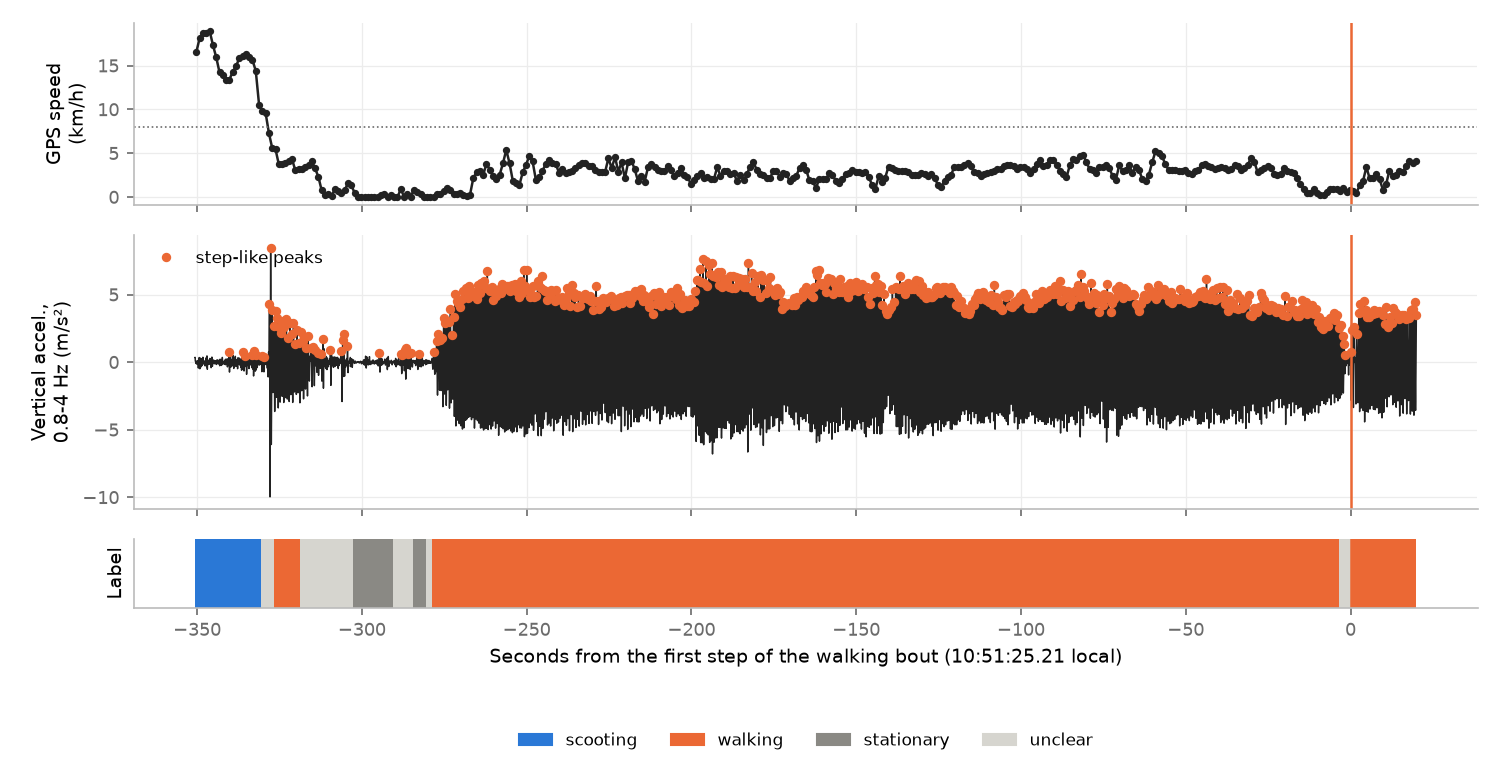
\includegraphics[width=\linewidth]{appendix/2026-10-07_1037_rec02_walk_onset_2.png}
\caption{Start of the second walking bout in ride 2 (first step 10:51:25.21), drawn as
Figure~\ref{fig:1}: GPS speed, band-passed vertical acceleration with step-like peaks, and
window labels.}\label{fig:Bonset2}
\end{figure}

\begin{figure}[htbp]
\centering
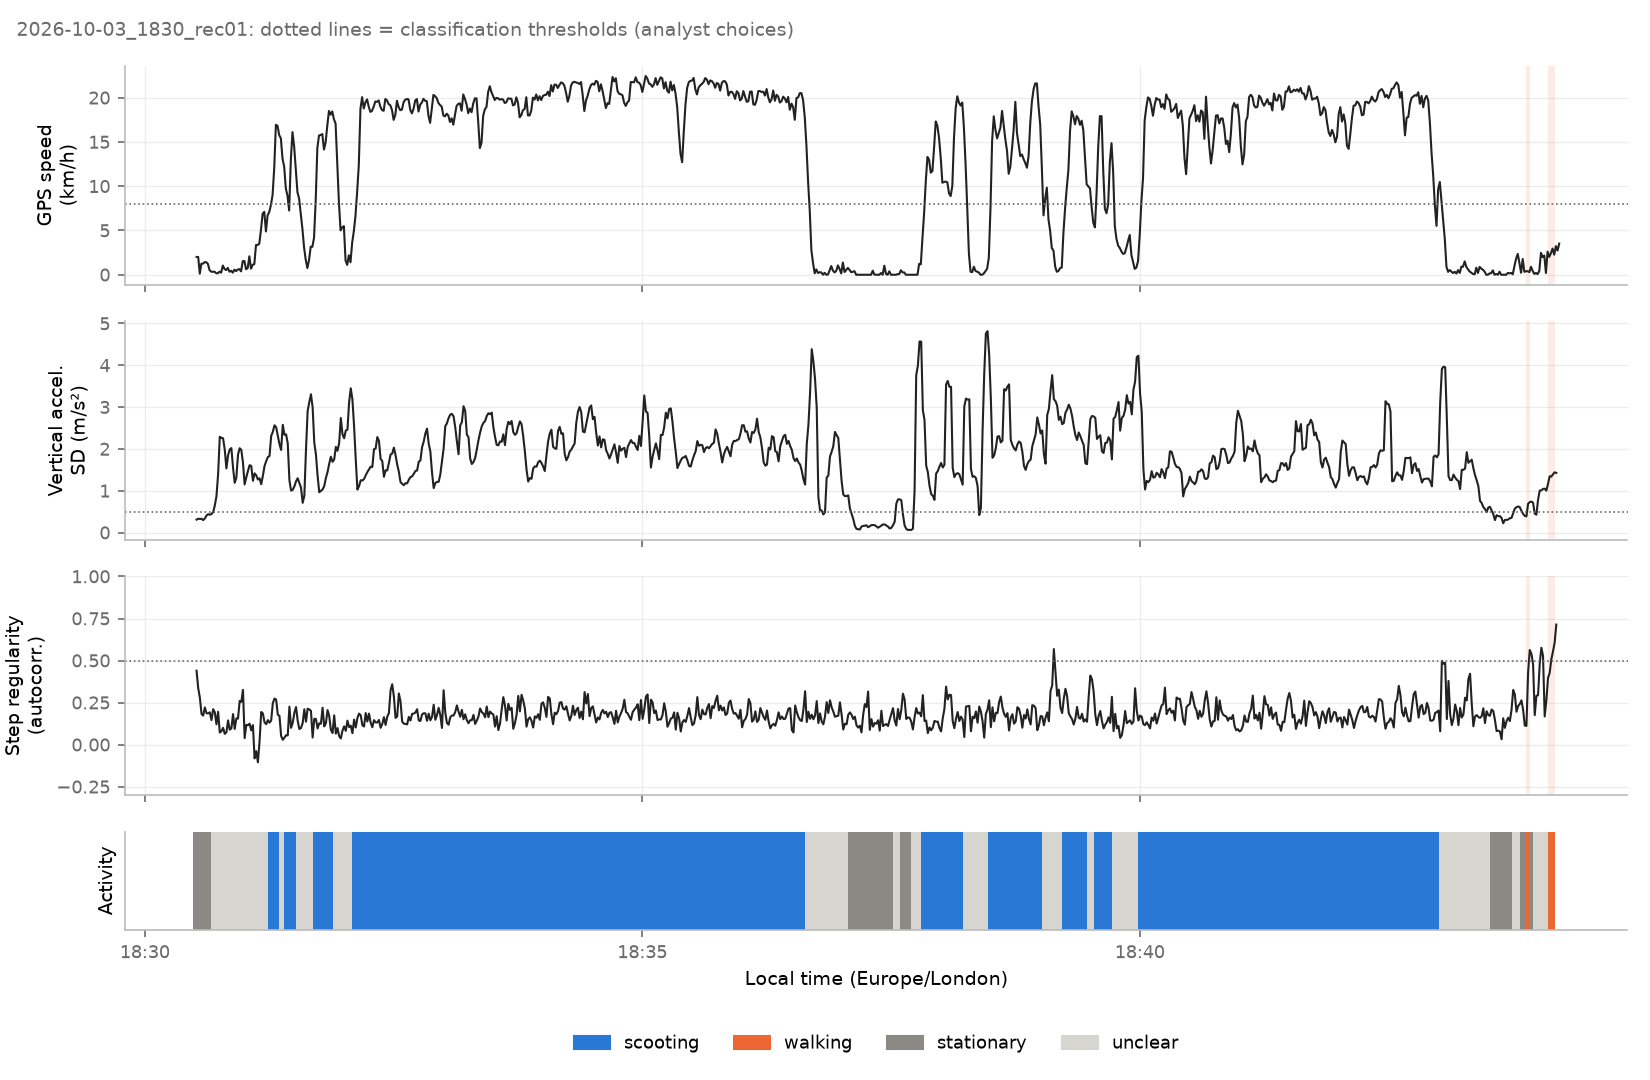
\includegraphics[width=\linewidth]{appendix/2026-10-03_1830_rec01_activity_timeline.png}
\caption{Ride 1: GPS speed, vertical acceleration SD, step regularity and activity
labels. Dotted lines: thresholds.}\label{fig:B1}
\end{figure}

\begin{figure}[htbp]
\centering
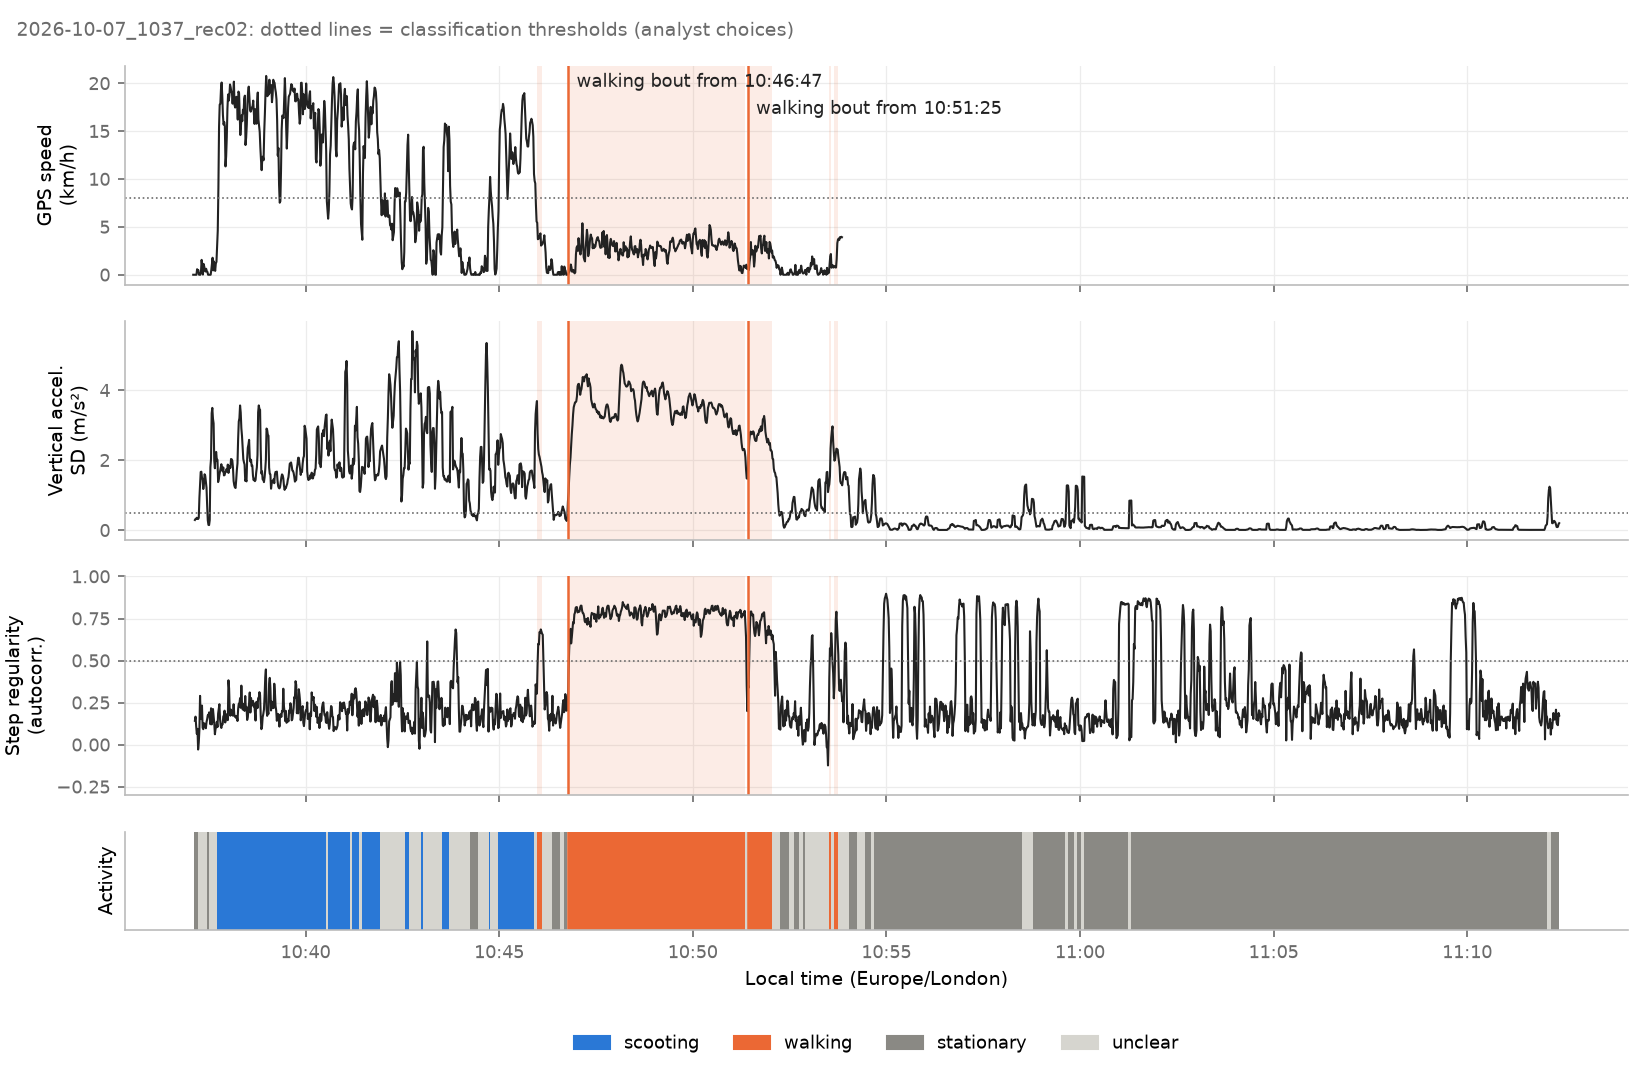
\includegraphics[width=\linewidth]{appendix/2026-10-07_1037_rec02_activity_timeline.png}
\caption{Ride 2: the ride, the walk from 10:46:47 and the phone at rest afterwards.
The repeated high step-regularity values after the walk come with almost no power in the
step band: a small periodic vibration, which the step-band rule correctly rejects.}\label{fig:B2}
\end{figure}

\begin{figure}[htbp]
\centering
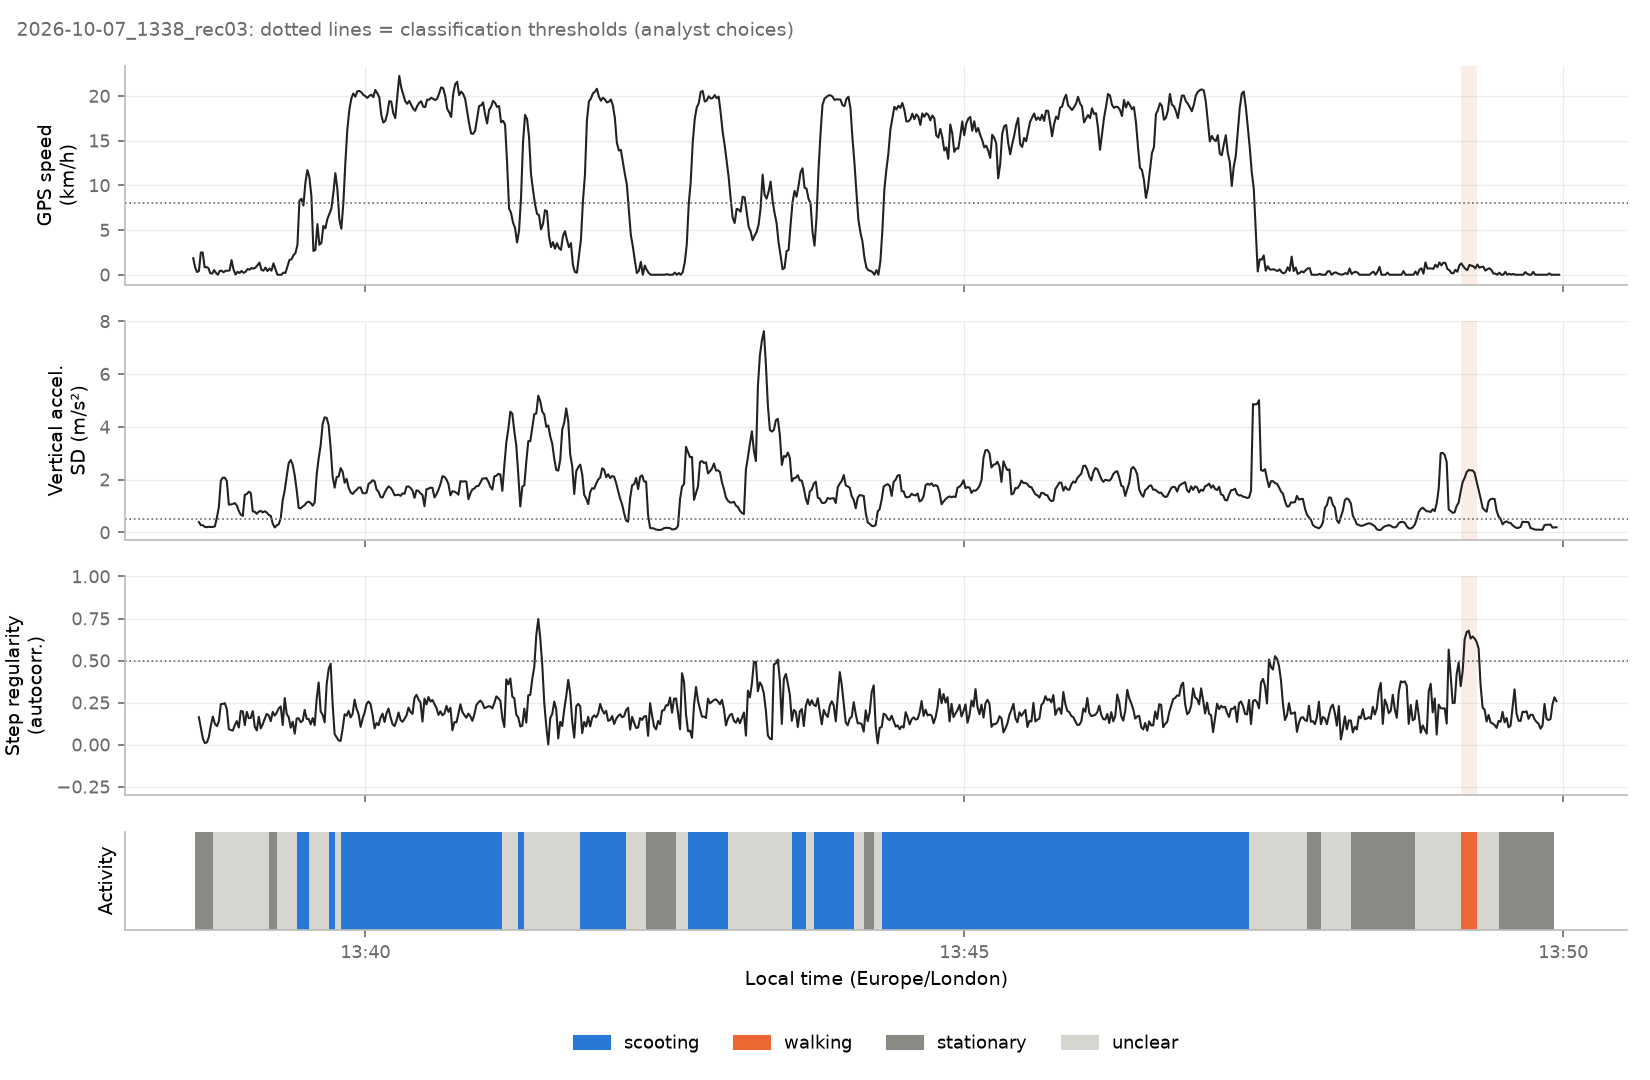
\includegraphics[width=\linewidth]{appendix/2026-10-07_1338_rec03_activity_timeline.png}
\caption{Ride 3.}\label{fig:B3}
\end{figure}


\section{Visual check of spots in street-level imagery}\label{visual-check-of-spots-in-street-level-imagery}

% SPOT_CHECK.md; outputs/combined/spot_links.csv

Table~\ref{tab:C1} lists the spots with links that open Google Street View at the spot,
facing the direction of travel and tilted 25° towards the road, a Google Maps pin, and
Mapillary imagery (the full list of all 33 spots, with the same links, is in the
supplementary file \texttt{spot\_links.csv}). The links use Google's documented Maps URLs,
which need no API key \autocite{googlemapsurls}; no imagery is downloaded, and no Street
View images are reproduced here, as Google does not permit their use in print. Open imagery was checked first:
Panoramax \autocite{panoramax} had no photos in the study area, and KartaView \autocite{kartaview} had
five photos near spot P1, from 2017 and 2021, too old to show the current surface.

Rules fixed before checking: record the imagery date shown in the viewer; record what is
visible within about 15 m of the spot (the phone's median GPS accuracy was 11--14 m) as
one or more of \emph{pothole}, \emph{crack or broken surface}, \emph{patched or repaired surface},
\emph{drain or manhole cover}, \emph{kerb or dropped kerb}, \emph{speed hump or raised table},
\emph{nothing visible}, \emph{no imagery}; do not change the categories once started. Imagery
dates differ from the ride dates, so a visible feature supports an impact but a clean
image does not rule a defect out.

\textbf{Results:} pending.

% Generated by scripts/paper_part_a.py (spot_table_tex) from outputs/combined/spot_links.csv;
% do not edit by hand. Styled after outputs/combined/spot_links.html.
\begin{landscape}
\footnotesize\arrayrulecolor{rulegray}
\setlength{\LTpre}{3pt}\setlength{\LTpost}{8pt}
\captionof{table}{Impact spots, most important first, as in the project's spot list. Links open Google Street View at the spot facing the direction of travel (tilted towards the road), a Google Maps pin, and Mapillary imagery. On paper, scan the QR code to open the same Street View, or enter the coordinates in any map. FixMyStreet: nearest road-surface report made in the 365 days before the ride (within 25 m, or the nearest). Spots P9, P16, P30, P31 lie in the hidden first or last 200 m of a route and are not listed, for privacy; they are included in all counts and in the tier totals.}\label{tab:C1}
\vspace{6pt}

\noindent{\normalsize\bfseries Tier 1: Hit on 2+ separate rides (10)}\par\nopagebreak
\begin{longtable}{@{}p{9mm} >{\raggedleft\arraybackslash}p{11mm} >{\raggedleft\arraybackslash}p{8mm} >{\raggedleft\arraybackslash}p{9mm} p{20mm} p{38mm} p{36mm} >{\raggedright\arraybackslash}p{31mm} >{\raggedright\arraybackslash}p{33mm} >{\centering\arraybackslash}p{14mm}@{}}
\toprule
Spot & Impacts & Rides & Max g & Road & Open & FixMyStreet (recent) & Location & Events (recording\#impact) & Scan \\
\midrule
\endfirsthead
\toprule
Spot & Impacts & Rides & Max g & Road & Open & FixMyStreet (recent) & Location & Events (recording\#impact) & Scan \\
\midrule
\endhead
\textbf{P1} & 6 & 3 & 2.24 & Marston Road & \href{https://www.google.com/maps/@?api=1\&map_action=pano\&viewpoint=51.754270,-1.235883\&heading=10\&pitch=-25\&fov=80}{Street View}\,\textperiodcentered\, \href{https://www.google.com/maps/search/?api=1\&query=51.754270,-1.235883}{Map}\,\textperiodcentered\, \href{https://www.mapillary.com/app/?lat=51.754270\&lng=-1.235883\&z=19}{Mapillary} & \textcolor{gray}{none $\leq$ 25 m (nearest \href{https://www.fixmystreet.com/report/9608286}{60 m})} & \textcolor{gray}{51.75427, −1.23588 \textperiodcentered{} \mbox{facing 10°}} & \textcolor{gray}{rec01\#31; rec02\#8; rec03\#17; rec03\#18; rec03\#19; rec03\#20} & \raisebox{-0.92\height}{\qrcode[height=13mm,level=L,nolink]{https://www.google.com/maps/@?api=1\&map_action=pano\&viewpoint=51.754270,-1.235883\&heading=10\&pitch=-25\&fov=80}} \\ \specialrule{0.2pt}{1pt}{1pt}
\textbf{P2} & 6 & 3 & 1.47 & Marston Road & \href{https://www.google.com/maps/@?api=1\&map_action=pano\&viewpoint=51.752684,-1.236654\&heading=27\&pitch=-25\&fov=80}{Street View}\,\textperiodcentered\, \href{https://www.google.com/maps/search/?api=1\&query=51.752684,-1.236654}{Map}\,\textperiodcentered\, \href{https://www.mapillary.com/app/?lat=51.752684\&lng=-1.236654\&z=19}{Mapillary} & \textcolor{gray}{none $\leq$ 25 m (nearest \href{https://www.fixmystreet.com/report/8694180}{44 m})} & \textcolor{gray}{51.75268, −1.23665 \textperiodcentered{} \mbox{facing 27°}} & \textcolor{gray}{rec01\#30; rec02\#9; rec02\#10; rec02\#11; rec02\#12; rec03\#16} & \raisebox{-0.92\height}{\qrcode[height=13mm,level=L,nolink]{https://www.google.com/maps/@?api=1\&map_action=pano\&viewpoint=51.752684,-1.236654\&heading=27\&pitch=-25\&fov=80}} \\ \specialrule{0.2pt}{1pt}{1pt}
\textbf{P3} & 19 & 2 & 2.25 & Other roads & \href{https://www.google.com/maps/@?api=1\&map_action=pano\&viewpoint=51.750235,-1.242534\&heading=261\&pitch=-25\&fov=80}{Street View}\,\textperiodcentered\, \href{https://www.google.com/maps/search/?api=1\&query=51.750235,-1.242534}{Map}\,\textperiodcentered\, \href{https://www.mapillary.com/app/?lat=51.750235\&lng=-1.242534\&z=19}{Mapillary} & report \href{https://www.fixmystreet.com/report/9029624}{5 m} (closed) & \textcolor{gray}{51.75024, −1.24253 \textperiodcentered{} \mbox{facing 261°}} & \textcolor{gray}{rec02\#25; rec02\#26; rec02\#27; rec02\#28; rec02\#29; rec02\#30; rec02\#31; rec02\#32; rec02\#33; rec02\#34; rec02\#35; rec02\#36; rec02\#37; rec02\#38; rec03\#1; rec03\#2; rec03\#3; rec03\#4; rec03\#5} & \raisebox{-0.92\height}{\qrcode[height=13mm,level=L,nolink]{https://www.google.com/maps/@?api=1\&map_action=pano\&viewpoint=51.750235,-1.242534\&heading=261\&pitch=-25\&fov=80}} \\ \specialrule{0.2pt}{1pt}{1pt}
\textbf{P4} & 10 & 2 & 6.28 & Other roads & \href{https://www.google.com/maps/@?api=1\&map_action=pano\&viewpoint=51.750849,-1.238775\&heading=218\&pitch=-25\&fov=80}{Street View}\,\textperiodcentered\, \href{https://www.google.com/maps/search/?api=1\&query=51.750849,-1.238775}{Map}\,\textperiodcentered\, \href{https://www.mapillary.com/app/?lat=51.750849\&lng=-1.238775\&z=19}{Mapillary} & report \href{https://www.fixmystreet.com/report/9436309}{8 m} (fixed) & \textcolor{gray}{51.75085, −1.23877 \textperiodcentered{} \mbox{facing 218°}} & \textcolor{gray}{rec02\#18; rec02\#19; rec02\#20; rec02\#21; rec02\#22; rec03\#9; rec03\#10; rec03\#11; rec03\#12; rec03\#13} & \raisebox{-0.92\height}{\qrcode[height=13mm,level=L,nolink]{https://www.google.com/maps/@?api=1\&map_action=pano\&viewpoint=51.750849,-1.238775\&heading=218\&pitch=-25\&fov=80}} \\ \specialrule{0.2pt}{1pt}{1pt}
\textbf{P5} & 9 & 2 & 1.79 & Marston Road & \href{https://www.google.com/maps/@?api=1\&map_action=pano\&viewpoint=51.756868,-1.235505\&heading=355\&pitch=-25\&fov=80}{Street View}\,\textperiodcentered\, \href{https://www.google.com/maps/search/?api=1\&query=51.756868,-1.235505}{Map}\,\textperiodcentered\, \href{https://www.mapillary.com/app/?lat=51.756868\&lng=-1.235505\&z=19}{Mapillary} & \textcolor{gray}{none $\leq$ 25 m (nearest \href{https://www.fixmystreet.com/report/9608286}{121 m})} & \textcolor{gray}{51.75687, −1.23551 \textperiodcentered{} \mbox{facing 355°}} & \textcolor{gray}{rec01\#33; rec01\#34; rec01\#35; rec01\#36; rec01\#37; rec02\#4; rec02\#5; rec02\#6; rec02\#7} & \raisebox{-0.92\height}{\qrcode[height=13mm,level=L,nolink]{https://www.google.com/maps/@?api=1\&map_action=pano\&viewpoint=51.756868,-1.235505\&heading=355\&pitch=-25\&fov=80}} \\ \specialrule{0.2pt}{1pt}{1pt}
\textbf{P6} & 4 & 2 & 1.85 & Other roads & \href{https://www.google.com/maps/@?api=1\&map_action=pano\&viewpoint=51.750594,-1.239934\&heading=249\&pitch=-25\&fov=80}{Street View}\,\textperiodcentered\, \href{https://www.google.com/maps/search/?api=1\&query=51.750594,-1.239934}{Map}\,\textperiodcentered\, \href{https://www.mapillary.com/app/?lat=51.750594\&lng=-1.239934\&z=19}{Mapillary} & report \href{https://www.fixmystreet.com/report/9850727}{8 m} (closed) & \textcolor{gray}{51.75059, −1.23993 \textperiodcentered{} \mbox{facing 249°}} & \textcolor{gray}{rec02\#23; rec02\#24; rec03\#7; rec03\#8} & \raisebox{-0.92\height}{\qrcode[height=13mm,level=L,nolink]{https://www.google.com/maps/@?api=1\&map_action=pano\&viewpoint=51.750594,-1.239934\&heading=249\&pitch=-25\&fov=80}} \\ \specialrule{0.2pt}{1pt}{1pt}
\textbf{P7} & 3 & 2 & 1.17 & Marston Road & \href{https://www.google.com/maps/@?api=1\&map_action=pano\&viewpoint=51.752081,-1.236996\&heading=180\&pitch=-25\&fov=80}{Street View}\,\textperiodcentered\, \href{https://www.google.com/maps/search/?api=1\&query=51.752081,-1.236996}{Map}\,\textperiodcentered\, \href{https://www.mapillary.com/app/?lat=51.752081\&lng=-1.236996\&z=19}{Mapillary} & report \href{https://www.fixmystreet.com/report/8512828}{8 m} (closed) & \textcolor{gray}{51.75208, −1.23700 \textperiodcentered{} \mbox{facing 180°}} & \textcolor{gray}{rec02\#13; rec02\#14; rec03\#15} & \raisebox{-0.92\height}{\qrcode[height=13mm,level=L,nolink]{https://www.google.com/maps/@?api=1\&map_action=pano\&viewpoint=51.752081,-1.236996\&heading=180\&pitch=-25\&fov=80}} \\ \specialrule{0.2pt}{1pt}{1pt}
\textbf{P8} & 2 & 2 & 2.80 & Other roads & \href{https://www.google.com/maps/@?api=1\&map_action=pano\&viewpoint=51.751550,-1.237717\&heading=52\&pitch=-25\&fov=80}{Street View}\,\textperiodcentered\, \href{https://www.google.com/maps/search/?api=1\&query=51.751550,-1.237717}{Map}\,\textperiodcentered\, \href{https://www.mapillary.com/app/?lat=51.751550\&lng=-1.237717\&z=19}{Mapillary} & \textcolor{gray}{none $\leq$ 25 m (nearest \href{https://www.fixmystreet.com/report/8336423}{38 m})} & \textcolor{gray}{51.75155, −1.23772 \textperiodcentered{} \mbox{facing 52°}} & \textcolor{gray}{rec01\#23; rec03\#14} & \raisebox{-0.92\height}{\qrcode[height=13mm,level=L,nolink]{https://www.google.com/maps/@?api=1\&map_action=pano\&viewpoint=51.751550,-1.237717\&heading=52\&pitch=-25\&fov=80}} \\ \specialrule{0.2pt}{1pt}{1pt}
\textbf{P10} & 2 & 2 & 1.34 & Marston Road & \href{https://www.google.com/maps/@?api=1\&map_action=pano\&viewpoint=51.757768,-1.235487\&heading=13\&pitch=-25\&fov=80}{Street View}\,\textperiodcentered\, \href{https://www.google.com/maps/search/?api=1\&query=51.757768,-1.235487}{Map}\,\textperiodcentered\, \href{https://www.mapillary.com/app/?lat=51.757768\&lng=-1.235487\&z=19}{Mapillary} & \textcolor{gray}{none $\leq$ 25 m (nearest \href{https://www.fixmystreet.com/report/8787376}{87 m})} & \textcolor{gray}{51.75777, −1.23549 \textperiodcentered{} \mbox{facing 13°}} & \textcolor{gray}{rec01\#38; rec03\#21} & \raisebox{-0.92\height}{\qrcode[height=13mm,level=L,nolink]{https://www.google.com/maps/@?api=1\&map_action=pano\&viewpoint=51.757768,-1.235487\&heading=13\&pitch=-25\&fov=80}} \\ \specialrule{0.2pt}{1pt}{1pt}
\end{longtable}

\needspace{9\baselineskip}
\noindent{\normalsize\bfseries Tier 2: 2+ impacts on one ride (10)}\par\nopagebreak
\begin{longtable}{@{}p{9mm} >{\raggedleft\arraybackslash}p{11mm} >{\raggedleft\arraybackslash}p{8mm} >{\raggedleft\arraybackslash}p{9mm} p{20mm} p{38mm} p{36mm} >{\raggedright\arraybackslash}p{31mm} >{\raggedright\arraybackslash}p{33mm} >{\centering\arraybackslash}p{14mm}@{}}
\toprule
Spot & Impacts & Rides & Max g & Road & Open & FixMyStreet (recent) & Location & Events (recording\#impact) & Scan \\
\midrule
\endfirsthead
\toprule
Spot & Impacts & Rides & Max g & Road & Open & FixMyStreet (recent) & Location & Events (recording\#impact) & Scan \\
\midrule
\endhead
\textbf{P11} & 3 & 1 & 2.87 & Morrell Avenue & \href{https://www.google.com/maps/@?api=1\&map_action=pano\&viewpoint=51.751237,-1.237962\&heading=224\&pitch=-25\&fov=80}{Street View}\,\textperiodcentered\, \href{https://www.google.com/maps/search/?api=1\&query=51.751237,-1.237962}{Map}\,\textperiodcentered\, \href{https://www.mapillary.com/app/?lat=51.751237\&lng=-1.237962\&z=19}{Mapillary} & report \href{https://www.fixmystreet.com/report/9495439}{12 m} (closed) & \textcolor{gray}{51.75124, −1.23796 \textperiodcentered{} \mbox{facing 224°}} & \textcolor{gray}{rec02\#15; rec02\#16; rec02\#17} & \raisebox{-0.92\height}{\qrcode[height=13mm,level=L,nolink]{https://www.google.com/maps/@?api=1\&map_action=pano\&viewpoint=51.751237,-1.237962\&heading=224\&pitch=-25\&fov=80}} \\ \specialrule{0.2pt}{1pt}{1pt}
\textbf{P12} & 3 & 1 & 2.68 & Other roads & \href{https://www.google.com/maps/@?api=1\&map_action=pano\&viewpoint=51.752220,-1.237662\&heading=286\&pitch=-25\&fov=80}{Street View}\,\textperiodcentered\, \href{https://www.google.com/maps/search/?api=1\&query=51.752220,-1.237662}{Map}\,\textperiodcentered\, \href{https://www.mapillary.com/app/?lat=51.752220\&lng=-1.237662\&z=19}{Mapillary} & report \href{https://www.fixmystreet.com/report/8666347}{6 m} (fixed) & \textcolor{gray}{51.75222, −1.23766 \textperiodcentered{} \mbox{facing 286°}} & \textcolor{gray}{rec01\#24; rec01\#28; rec01\#29} & \raisebox{-0.92\height}{\qrcode[height=13mm,level=L,nolink]{https://www.google.com/maps/@?api=1\&map_action=pano\&viewpoint=51.752220,-1.237662\&heading=286\&pitch=-25\&fov=80}} \\ \specialrule{0.2pt}{1pt}{1pt}
\textbf{P13} & 3 & 1 & 1.48 & Morrell Avenue & \href{https://www.google.com/maps/@?api=1\&map_action=pano\&viewpoint=51.749809,-1.230171\&heading=267\&pitch=-25\&fov=80}{Street View}\,\textperiodcentered\, \href{https://www.google.com/maps/search/?api=1\&query=51.749809,-1.230171}{Map}\,\textperiodcentered\, \href{https://www.mapillary.com/app/?lat=51.749809\&lng=-1.230171\&z=19}{Mapillary} & \textcolor{gray}{none $\leq$ 25 m (nearest \href{https://www.fixmystreet.com/report/9012527}{113 m})} & \textcolor{gray}{51.74981, −1.23017 \textperiodcentered{} \mbox{facing 267°}} & \textcolor{gray}{rec01\#13; rec01\#14; rec01\#15} & \raisebox{-0.92\height}{\qrcode[height=13mm,level=L,nolink]{https://www.google.com/maps/@?api=1\&map_action=pano\&viewpoint=51.749809,-1.230171\&heading=267\&pitch=-25\&fov=80}} \\ \specialrule{0.2pt}{1pt}{1pt}
\textbf{P14} & 3 & 1 & 1.17 & Other roads & \href{https://www.google.com/maps/@?api=1\&map_action=pano\&viewpoint=51.751621,-1.222891\&heading=226\&pitch=-25\&fov=80}{Street View}\,\textperiodcentered\, \href{https://www.google.com/maps/search/?api=1\&query=51.751621,-1.222891}{Map}\,\textperiodcentered\, \href{https://www.mapillary.com/app/?lat=51.751621\&lng=-1.222891\&z=19}{Mapillary} & \textcolor{gray}{none $\leq$ 25 m (nearest \href{https://www.fixmystreet.com/report/8744515}{118 m})} & \textcolor{gray}{51.75162, −1.22289 \textperiodcentered{} \mbox{facing 226°}} & \textcolor{gray}{rec01\#6; rec01\#7; rec01\#8} & \raisebox{-0.92\height}{\qrcode[height=13mm,level=L,nolink]{https://www.google.com/maps/@?api=1\&map_action=pano\&viewpoint=51.751621,-1.222891\&heading=226\&pitch=-25\&fov=80}} \\ \specialrule{0.2pt}{1pt}{1pt}
\textbf{P15} & 2 & 1 & 1.37 & Other roads & \href{https://www.google.com/maps/@?api=1\&map_action=pano\&viewpoint=51.752562,-1.238892\&heading=293\&pitch=-25\&fov=80}{Street View}\,\textperiodcentered\, \href{https://www.google.com/maps/search/?api=1\&query=51.752562,-1.238892}{Map}\,\textperiodcentered\, \href{https://www.mapillary.com/app/?lat=51.752562\&lng=-1.238892\&z=19}{Mapillary} & \textcolor{gray}{none $\leq$ 25 m (nearest \href{https://www.fixmystreet.com/report/8666347}{73 m})} & \textcolor{gray}{51.75256, −1.23889 \textperiodcentered{} \mbox{facing 293°}} & \textcolor{gray}{rec01\#25; rec01\#26} & \raisebox{-0.92\height}{\qrcode[height=13mm,level=L,nolink]{https://www.google.com/maps/@?api=1\&map_action=pano\&viewpoint=51.752562,-1.238892\&heading=293\&pitch=-25\&fov=80}} \\ \specialrule{0.2pt}{1pt}{1pt}
\textbf{P17} & 2 & 1 & 1.31 & Morrell Avenue & \href{https://www.google.com/maps/@?api=1\&map_action=pano\&viewpoint=51.749740,-1.231359\&heading=265\&pitch=-25\&fov=80}{Street View}\,\textperiodcentered\, \href{https://www.google.com/maps/search/?api=1\&query=51.749740,-1.231359}{Map}\,\textperiodcentered\, \href{https://www.mapillary.com/app/?lat=51.749740\&lng=-1.231359\&z=19}{Mapillary} & \textcolor{gray}{none $\leq$ 25 m (nearest \href{https://www.fixmystreet.com/report/9012527}{178 m})} & \textcolor{gray}{51.74974, −1.23136 \textperiodcentered{} \mbox{facing 265°}} & \textcolor{gray}{rec01\#16; rec01\#17} & \raisebox{-0.92\height}{\qrcode[height=13mm,level=L,nolink]{https://www.google.com/maps/@?api=1\&map_action=pano\&viewpoint=51.749740,-1.231359\&heading=265\&pitch=-25\&fov=80}} \\ \specialrule{0.2pt}{1pt}{1pt}
\textbf{P18} & 2 & 1 & 1.24 & Other roads & \href{https://www.google.com/maps/@?api=1\&map_action=pano\&viewpoint=51.751195,-1.223560\&heading=224\&pitch=-25\&fov=80}{Street View}\,\textperiodcentered\, \href{https://www.google.com/maps/search/?api=1\&query=51.751195,-1.223560}{Map}\,\textperiodcentered\, \href{https://www.mapillary.com/app/?lat=51.751195\&lng=-1.223560\&z=19}{Mapillary} & \textcolor{gray}{none $\leq$ 25 m (nearest \href{https://www.fixmystreet.com/report/9236232}{115 m})} & \textcolor{gray}{51.75120, −1.22356 \textperiodcentered{} \mbox{facing 224°}} & \textcolor{gray}{rec01\#9; rec01\#10} & \raisebox{-0.92\height}{\qrcode[height=13mm,level=L,nolink]{https://www.google.com/maps/@?api=1\&map_action=pano\&viewpoint=51.751195,-1.223560\&heading=224\&pitch=-25\&fov=80}} \\ \specialrule{0.2pt}{1pt}{1pt}
\textbf{P19} & 2 & 1 & 1.18 & Morrell Avenue & \href{https://www.google.com/maps/@?api=1\&map_action=pano\&viewpoint=51.749830,-1.233869\&heading=285\&pitch=-25\&fov=80}{Street View}\,\textperiodcentered\, \href{https://www.google.com/maps/search/?api=1\&query=51.749830,-1.233869}{Map}\,\textperiodcentered\, \href{https://www.mapillary.com/app/?lat=51.749830\&lng=-1.233869\&z=19}{Mapillary} & \textcolor{gray}{none $\leq$ 25 m (nearest \href{https://www.fixmystreet.com/report/9415948}{75 m})} & \textcolor{gray}{51.74983, −1.23387 \textperiodcentered{} \mbox{facing 285°}} & \textcolor{gray}{rec01\#18; rec01\#19} & \raisebox{-0.92\height}{\qrcode[height=13mm,level=L,nolink]{https://www.google.com/maps/@?api=1\&map_action=pano\&viewpoint=51.749830,-1.233869\&heading=285\&pitch=-25\&fov=80}} \\ \specialrule{0.2pt}{1pt}{1pt}
\textbf{P20} & 2 & 1 & 1.13 & Old Road & \href{https://www.google.com/maps/@?api=1\&map_action=pano\&viewpoint=51.753330,-1.218484\&heading=248\&pitch=-25\&fov=80}{Street View}\,\textperiodcentered\, \href{https://www.google.com/maps/search/?api=1\&query=51.753330,-1.218484}{Map}\,\textperiodcentered\, \href{https://www.mapillary.com/app/?lat=51.753330\&lng=-1.218484\&z=19}{Mapillary} & \textcolor{gray}{none $\leq$ 25 m (nearest \href{https://www.fixmystreet.com/report/8852037}{58 m})} & \textcolor{gray}{51.75333, −1.21848 \textperiodcentered{} \mbox{facing 248°}} & \textcolor{gray}{rec01\#3; rec01\#4} & \raisebox{-0.92\height}{\qrcode[height=13mm,level=L,nolink]{https://www.google.com/maps/@?api=1\&map_action=pano\&viewpoint=51.753330,-1.218484\&heading=248\&pitch=-25\&fov=80}} \\ \specialrule{0.2pt}{1pt}{1pt}
\end{longtable}

\needspace{9\baselineskip}
\noindent{\normalsize\bfseries Tier 3: Single impact (13)}\par\nopagebreak
\begin{longtable}{@{}p{9mm} >{\raggedleft\arraybackslash}p{11mm} >{\raggedleft\arraybackslash}p{8mm} >{\raggedleft\arraybackslash}p{9mm} p{20mm} p{38mm} p{36mm} >{\raggedright\arraybackslash}p{31mm} >{\raggedright\arraybackslash}p{33mm} >{\centering\arraybackslash}p{14mm}@{}}
\toprule
Spot & Impacts & Rides & Max g & Road & Open & FixMyStreet (recent) & Location & Events (recording\#impact) & Scan \\
\midrule
\endfirsthead
\toprule
Spot & Impacts & Rides & Max g & Road & Open & FixMyStreet (recent) & Location & Events (recording\#impact) & Scan \\
\midrule
\endhead
\textbf{P21} & 1 & 1 & 2.64 & Other roads & \href{https://www.google.com/maps/@?api=1\&map_action=pano\&viewpoint=51.749873,-1.244328\&heading=219\&pitch=-25\&fov=80}{Street View}\,\textperiodcentered\, \href{https://www.google.com/maps/search/?api=1\&query=51.749873,-1.244328}{Map}\,\textperiodcentered\, \href{https://www.mapillary.com/app/?lat=51.749873\&lng=-1.244328\&z=19}{Mapillary} & report \href{https://www.fixmystreet.com/report/8891248}{23 m} (fixed) & \textcolor{gray}{51.74987, −1.24433 \textperiodcentered{} \mbox{facing 219°}} & \textcolor{gray}{rec02\#39} & \raisebox{-0.92\height}{\qrcode[height=13mm,level=L,nolink]{https://www.google.com/maps/@?api=1\&map_action=pano\&viewpoint=51.749873,-1.244328\&heading=219\&pitch=-25\&fov=80}} \\ \specialrule{0.2pt}{1pt}{1pt}
\textbf{P22} & 1 & 1 & 1.73 & Other roads & \href{https://www.google.com/maps/@?api=1\&map_action=pano\&viewpoint=51.752107,-1.222087\&heading=225\&pitch=-25\&fov=80}{Street View}\,\textperiodcentered\, \href{https://www.google.com/maps/search/?api=1\&query=51.752107,-1.222087}{Map}\,\textperiodcentered\, \href{https://www.mapillary.com/app/?lat=51.752107\&lng=-1.222087\&z=19}{Mapillary} & \textcolor{gray}{none $\leq$ 25 m (nearest \href{https://www.fixmystreet.com/report/8744515}{52 m})} & \textcolor{gray}{51.75211, −1.22209 \textperiodcentered{} \mbox{facing 225°}} & \textcolor{gray}{rec01\#5} & \raisebox{-0.92\height}{\qrcode[height=13mm,level=L,nolink]{https://www.google.com/maps/@?api=1\&map_action=pano\&viewpoint=51.752107,-1.222087\&heading=225\&pitch=-25\&fov=80}} \\ \specialrule{0.2pt}{1pt}{1pt}
\textbf{P23} & 1 & 1 & 1.39 & Marston Road & \href{https://www.google.com/maps/@?api=1\&map_action=pano\&viewpoint=51.755210,-1.235670\&heading=8\&pitch=-25\&fov=80}{Street View}\,\textperiodcentered\, \href{https://www.google.com/maps/search/?api=1\&query=51.755210,-1.235670}{Map}\,\textperiodcentered\, \href{https://www.mapillary.com/app/?lat=51.755210\&lng=-1.235670\&z=19}{Mapillary} & report \href{https://www.fixmystreet.com/report/9608286}{5 m} (closed) & \textcolor{gray}{51.75521, −1.23567 \textperiodcentered{} \mbox{facing 8°}} & \textcolor{gray}{rec01\#32} & \raisebox{-0.92\height}{\qrcode[height=13mm,level=L,nolink]{https://www.google.com/maps/@?api=1\&map_action=pano\&viewpoint=51.755210,-1.235670\&heading=8\&pitch=-25\&fov=80}} \\ \specialrule{0.2pt}{1pt}{1pt}
\textbf{P24} & 1 & 1 & 1.23 & Morrell Avenue & \href{https://www.google.com/maps/@?api=1\&map_action=pano\&viewpoint=51.750129,-1.235206\&heading=308\&pitch=-25\&fov=80}{Street View}\,\textperiodcentered\, \href{https://www.google.com/maps/search/?api=1\&query=51.750129,-1.235206}{Map}\,\textperiodcentered\, \href{https://www.mapillary.com/app/?lat=51.750129\&lng=-1.235206\&z=19}{Mapillary} & \textcolor{gray}{none $\leq$ 25 m (nearest \href{https://www.fixmystreet.com/report/9415948}{73 m})} & \textcolor{gray}{51.75013, −1.23521 \textperiodcentered{} \mbox{facing 308°}} & \textcolor{gray}{rec01\#20} & \raisebox{-0.92\height}{\qrcode[height=13mm,level=L,nolink]{https://www.google.com/maps/@?api=1\&map_action=pano\&viewpoint=51.750129,-1.235206\&heading=308\&pitch=-25\&fov=80}} \\ \specialrule{0.2pt}{1pt}{1pt}
\textbf{P25} & 1 & 1 & 1.19 & Morrell Avenue & \href{https://www.google.com/maps/@?api=1\&map_action=pano\&viewpoint=51.750147,-1.226823\&heading=251\&pitch=-25\&fov=80}{Street View}\,\textperiodcentered\, \href{https://www.google.com/maps/search/?api=1\&query=51.750147,-1.226823}{Map}\,\textperiodcentered\, \href{https://www.mapillary.com/app/?lat=51.750147\&lng=-1.226823\&z=19}{Mapillary} & \textcolor{gray}{none $\leq$ 25 m (nearest \href{https://www.fixmystreet.com/report/8659259}{115 m})} & \textcolor{gray}{51.75015, −1.22682 \textperiodcentered{} \mbox{facing 251°}} & \textcolor{gray}{rec01\#11} & \raisebox{-0.92\height}{\qrcode[height=13mm,level=L,nolink]{https://www.google.com/maps/@?api=1\&map_action=pano\&viewpoint=51.750147,-1.226823\&heading=251\&pitch=-25\&fov=80}} \\ \specialrule{0.2pt}{1pt}{1pt}
\textbf{P26} & 1 & 1 & 1.17 & Other roads & \href{https://www.google.com/maps/@?api=1\&map_action=pano\&viewpoint=51.752416,-1.238294\&heading=111\&pitch=-25\&fov=80}{Street View}\,\textperiodcentered\, \href{https://www.google.com/maps/search/?api=1\&query=51.752416,-1.238294}{Map}\,\textperiodcentered\, \href{https://www.mapillary.com/app/?lat=51.752416\&lng=-1.238294\&z=19}{Mapillary} & \textcolor{gray}{none $\leq$ 25 m (nearest \href{https://www.fixmystreet.com/report/8666347}{31 m})} & \textcolor{gray}{51.75242, −1.23829 \textperiodcentered{} \mbox{facing 111°}} & \textcolor{gray}{rec01\#27} & \raisebox{-0.92\height}{\qrcode[height=13mm,level=L,nolink]{https://www.google.com/maps/@?api=1\&map_action=pano\&viewpoint=51.752416,-1.238294\&heading=111\&pitch=-25\&fov=80}} \\ \specialrule{0.2pt}{1pt}{1pt}
\textbf{P27} & 1 & 1 & 1.15 & Marston Road & \href{https://www.google.com/maps/@?api=1\&map_action=pano\&viewpoint=51.758061,-1.235642\&heading=176\&pitch=-25\&fov=80}{Street View}\,\textperiodcentered\, \href{https://www.google.com/maps/search/?api=1\&query=51.758061,-1.235642}{Map}\,\textperiodcentered\, \href{https://www.mapillary.com/app/?lat=51.758061\&lng=-1.235642\&z=19}{Mapillary} & \textcolor{gray}{none $\leq$ 25 m (nearest \href{https://www.fixmystreet.com/report/9020598}{249 m})} & \textcolor{gray}{51.75806, −1.23564 \textperiodcentered{} \mbox{facing 176°}} & \textcolor{gray}{rec02\#3} & \raisebox{-0.92\height}{\qrcode[height=13mm,level=L,nolink]{https://www.google.com/maps/@?api=1\&map_action=pano\&viewpoint=51.758061,-1.235642\&heading=176\&pitch=-25\&fov=80}} \\ \specialrule{0.2pt}{1pt}{1pt}
\textbf{P28} & 1 & 1 & 1.13 & Morrell Avenue & \href{https://www.google.com/maps/@?api=1\&map_action=pano\&viewpoint=51.750307,-1.235572\&heading=304\&pitch=-25\&fov=80}{Street View}\,\textperiodcentered\, \href{https://www.google.com/maps/search/?api=1\&query=51.750307,-1.235572}{Map}\,\textperiodcentered\, \href{https://www.mapillary.com/app/?lat=51.750307\&lng=-1.235572\&z=19}{Mapillary} & \textcolor{gray}{none $\leq$ 25 m (nearest \href{https://www.fixmystreet.com/report/8668106}{68 m})} & \textcolor{gray}{51.75031, −1.23557 \textperiodcentered{} \mbox{facing 304°}} & \textcolor{gray}{rec01\#21} & \raisebox{-0.92\height}{\qrcode[height=13mm,level=L,nolink]{https://www.google.com/maps/@?api=1\&map_action=pano\&viewpoint=51.750307,-1.235572\&heading=304\&pitch=-25\&fov=80}} \\ \specialrule{0.2pt}{1pt}{1pt}
\textbf{P29} & 1 & 1 & 1.12 & Morrell Avenue & \href{https://www.google.com/maps/@?api=1\&map_action=pano\&viewpoint=51.750943,-1.236971\&heading=297\&pitch=-25\&fov=80}{Street View}\,\textperiodcentered\, \href{https://www.google.com/maps/search/?api=1\&query=51.750943,-1.236971}{Map}\,\textperiodcentered\, \href{https://www.mapillary.com/app/?lat=51.750943\&lng=-1.236971\&z=19}{Mapillary} & \textcolor{gray}{none $\leq$ 25 m (nearest \href{https://www.fixmystreet.com/report/9052222}{65 m})} & \textcolor{gray}{51.75094, −1.23697 \textperiodcentered{} \mbox{facing 297°}} & \textcolor{gray}{rec01\#22} & \raisebox{-0.92\height}{\qrcode[height=13mm,level=L,nolink]{https://www.google.com/maps/@?api=1\&map_action=pano\&viewpoint=51.750943,-1.236971\&heading=297\&pitch=-25\&fov=80}} \\ \specialrule{0.2pt}{1pt}{1pt}
\textbf{P32} & 1 & 1 & 1.05 & Other roads & \href{https://www.google.com/maps/@?api=1\&map_action=pano\&viewpoint=51.750375,-1.241276\&heading=80\&pitch=-25\&fov=80}{Street View}\,\textperiodcentered\, \href{https://www.google.com/maps/search/?api=1\&query=51.750375,-1.241276}{Map}\,\textperiodcentered\, \href{https://www.mapillary.com/app/?lat=51.750375\&lng=-1.241276\&z=19}{Mapillary} & \textcolor{gray}{none $\leq$ 25 m (nearest \href{https://www.fixmystreet.com/report/10069088}{68 m})} & \textcolor{gray}{51.75037, −1.24128 \textperiodcentered{} \mbox{facing 80°}} & \textcolor{gray}{rec03\#6} & \raisebox{-0.92\height}{\qrcode[height=13mm,level=L,nolink]{https://www.google.com/maps/@?api=1\&map_action=pano\&viewpoint=51.750375,-1.241276\&heading=80\&pitch=-25\&fov=80}} \\ \specialrule{0.2pt}{1pt}{1pt}
\textbf{P33} & 1 & 1 & 1.04 & Morrell Avenue & \href{https://www.google.com/maps/@?api=1\&map_action=pano\&viewpoint=51.750045,-1.227441\&heading=260\&pitch=-25\&fov=80}{Street View}\,\textperiodcentered\, \href{https://www.google.com/maps/search/?api=1\&query=51.750045,-1.227441}{Map}\,\textperiodcentered\, \href{https://www.mapillary.com/app/?lat=51.750045\&lng=-1.227441\&z=19}{Mapillary} & \textcolor{gray}{none $\leq$ 25 m (nearest \href{https://www.fixmystreet.com/report/9012527}{131 m})} & \textcolor{gray}{51.75005, −1.22744 \textperiodcentered{} \mbox{facing 260°}} & \textcolor{gray}{rec01\#12} & \raisebox{-0.92\height}{\qrcode[height=13mm,level=L,nolink]{https://www.google.com/maps/@?api=1\&map_action=pano\&viewpoint=51.750045,-1.227441\&heading=260\&pitch=-25\&fov=80}} \\ \specialrule{0.2pt}{1pt}{1pt}
\end{longtable}

\arrayrulecolor{black}
\end{landscape}


% TODO: summarise outputs/combined/spot_links.csv by tier once checked

% Appendix D: road bumps (exploratory). Decided 2026-10-08: in the paper as an exploratory
% appendix only (revising the earlier "not in the paper"). Source: DOCUMENTATION.md 6.8,
% SIMULATION_METHODS.md 3.15 and 4.9; numbers from outputs/scooter_sim/[suspension/]bumps/
% (bump_fall_counts.csv, bump_rear_check_thresholds.csv) and keyframes/keyframes_runs.csv.

\section{Road bumps: an exploratory extension of the model}\label{app:bumps}

\textbf{Status.} These are exploratory model results, not findings about real scooters.
No bump was measured or identified on the rides, and the model's behaviour on bumps has
not been validated. Everything below describes what the simulation produced under its
assumed parameters (Table~\ref{tab:4}) and the analyst-chosen fall criteria
(section~\ref{dynamics-model}).

\textbf{Why bumps.} Raised obstacles, such as a utility cover or patch standing proud of
the surface, a lifted slab, a tree-root ridge or a traffic-calming hump, are a second
kind of road irregularity a rider may meet. Whether they matter for e-scooter riders in
practice is not tested here.

\textbf{What was simulated.} The dynamics model of section~\ref{dynamics-model}, unchanged
except for the road:
\begin{itemize}
\item \emph{Sharp-edged rectangular bumps}, 20--100 mm high, 300, 600 and 1000 mm long (the
  pothole lengths), with MuJoCo's contact. This idealised shape stands for defects: legal
  UK road humps may not have a vertical face above 6 mm \autocite{roadhumps1999}.
\item \emph{Round-top (circular-arc) humps}, 20--100 mm high, 3.7 m long, the round-top
  length reported as standard \autocite{tal2_96}, and 600 mm long (shorter than the 900 mm
  legal minimum, as might be found off the highway), with the profile contact.
\item The same sharp bumps with the profile contact, as a cross-check of the contact model.
\item Speeds of 15, 20 and 25 km/h, configurations 10/10, 12/10, 12/12 and 14/10, without
  and with the modelled front spring; and a rear-size check on the 300 mm sharp bump
  (heights 50--100 mm in 5 mm steps, seven configurations including larger rear wheels).
\end{itemize}
In the fall attribution, a fall is credited to the rear wheel if the rear wheel had
reached the bump's leading face before the fall criterion was met.

\begin{table}[htbp]
\centering\small
\caption{Number of runs meeting the fall criteria, per configuration (sharp bumps and
potholes: of 81 runs; round-top humps: of 54).}\label{tab:D1}
\begin{tabular}{@{}llrrrr@{}}
\toprule
Obstacle & Fork & 10/10 & 12/10 & 12/12 & 14/10 \\
\midrule
Pothole (sharp) & none & 15 & 14 & 14 & 11 \\
Sharp bump & none & 22 & 13 & 14 & 4 \\
Round-top hump & none & 0 & 0 & 0 & 0 \\
\addlinespace
Pothole (sharp) & front spring & 9 & 6 & 6 & 1 \\
Sharp bump & front spring & 1 & 2 & 1 & 2 \\
Round-top hump & front spring & 0 & 0 & 0 & 0 \\
\bottomrule
\end{tabular}
\end{table}

\begin{table}[htbp]
\centering\small
\caption{Rear-size check, 300 mm sharp bump: lowest bump height (mm, 5 mm steps) at which
the model met the fall criteria; -- = not met up to 100 mm.}\label{tab:D2}
\begin{tabular}{@{}llrrrrrrr@{}}
\toprule
Fork & Speed & 10/10 & 12/10 & 14/10 & 10/12 & 12/12 & 10/14 & 14/14 \\
\midrule
none & 15 km/h & 85 & 95 & -- & 85 & 95 & 85 & -- \\
none & 20 km/h & 80 & 90 & 100 & 80 & 90 & 80 & 100 \\
none & 25 km/h & 80 & 85 & 100 & 80 & 85 & 80 & 95 \\
\addlinespace
front spring & 15 km/h & 85 & 85 & 85 & 90 & 95 & -- & 100 \\
front spring & 20, 25 km/h & -- & -- & -- & -- & -- & -- & -- \\
\bottomrule
\end{tabular}
\end{table}

\textbf{Observations (model only).}
\begin{enumerate}
\item \emph{Without the front spring}, the current configuration met the fall criteria in
  more sharp-bump runs than pothole runs of the same dimensions (22 against 15 of 81;
  Table~\ref{tab:D1}). A plausible geometric explanation, not tested separately, is that a
  wheel meets the full height of a step but drops only part way into a short pothole.
  Fewer falls occurred with larger front wheels (22, 13 and 4 for 10, 12 and 14 in fronts);
  changing the rear size alone did not change the falling heights (Table~\ref{tab:D2}).
  Figure~\ref{fig:D1} shows one case.
\item \emph{With the front spring}, bump falls were rare: one or two runs per configuration,
  all on the 300 mm bump at 15 km/h. In each, the fall criteria were met after the rear
  wheel struck the bump's leading edge (Figure~\ref{fig:D2}). In the rear-size check, a
  larger rear wheel raised the falling height or prevented the fall (10/12: 90 mm; 12/12:
  95 mm; 14/14: 100 mm; 10/14: none up to 100 mm), while a larger front wheel alone did
  not (85 mm for 10/10, 12/10 and 14/10). This rests on very few runs (one bump length, one
  speed, differences of 5--15 mm, close to the 5 mm step) and on a model not validated
  for bumps. It is reported as an open question, whether rear-wheel size or rear
  suspension matters on scooters with a sprung front, not as evidence that larger rear
  wheels are more stable. It does indicate that the working hypothesis of this paper (the
  front wheel alone) may not hold for every type of obstacle.
\item No round-top hump run met the fall criteria in any configuration, consistent with,
  but not evidence for, guidance that humps can be ridden safely by cyclists and
  motorcyclists \autocite{tal7_96}; that guidance was not written for e-scooters. The
  short 600 mm hump gave large modelled speed losses at 15 km/h (up to 47\% with the
  fork).
\item The front spring changed the bump results much more than the pothole results (10/10:
  22 to 1 falls on bumps, 15 to 9 on potholes), so the bump results depend strongly on
  the assumed fork stiffness, damping and travel, which were not varied for bumps.
\end{enumerate}

\begin{figure}[htbp]
\centering
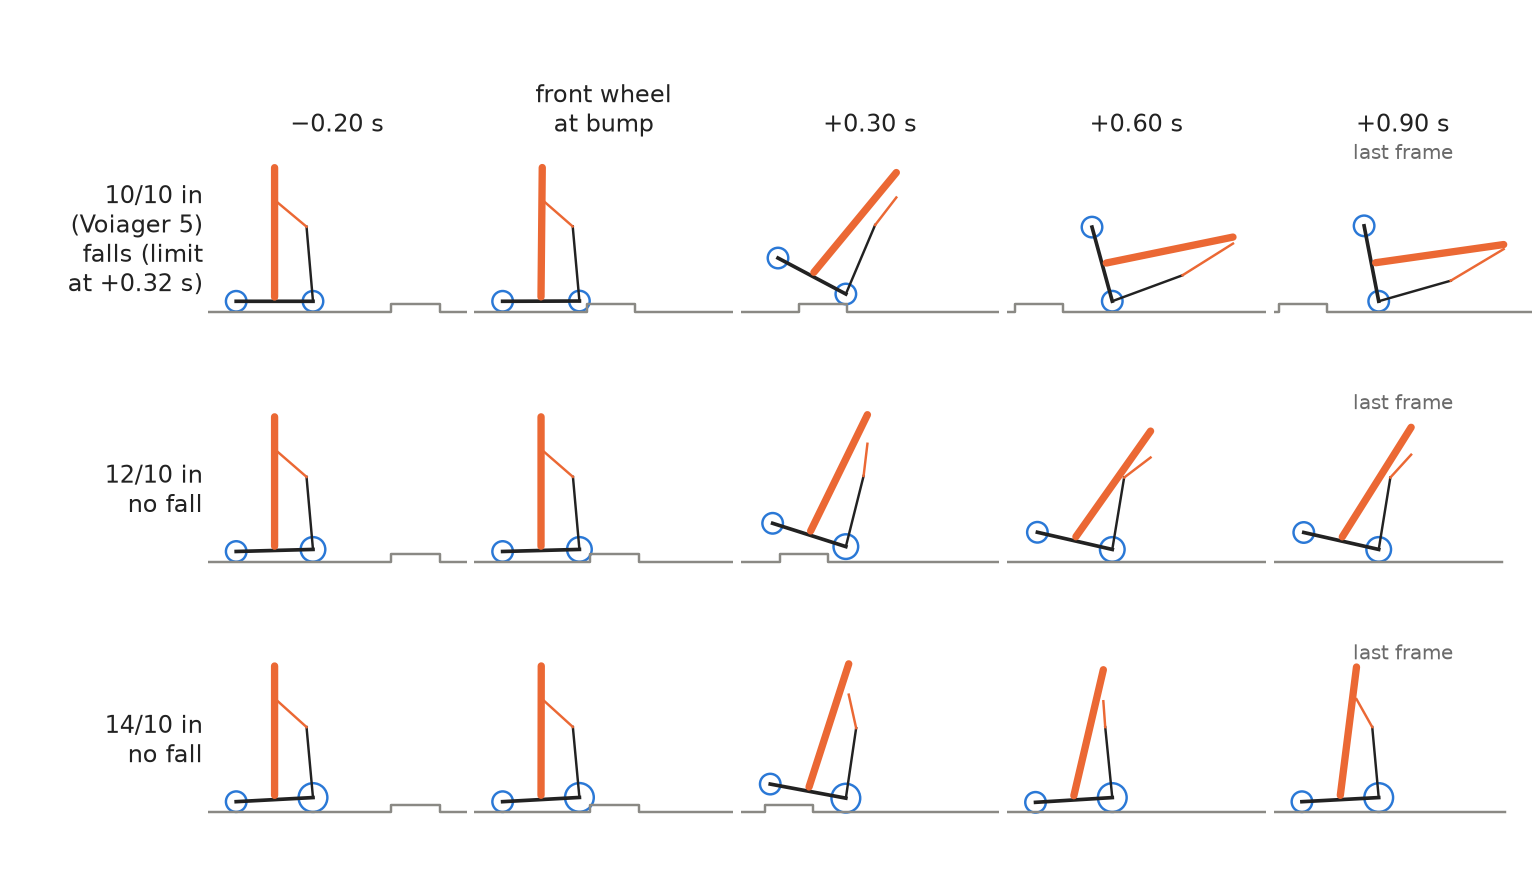
\includegraphics[width=\linewidth]{fig_d1_bump_keyframes.png}
\caption{Key frames, sharp-edged bump 90 mm high and 600 mm long at 20 km/h, model
without front suspension. Columns: the same moments in each row, relative to the front
wheel reaching the bump. The current configuration pitches forward after the front-wheel
strike; with 12 in and 14 in front wheels the model rolls over the bump. Drawn as in
Figure~\ref{fig:5}.}\label{fig:D1}
\end{figure}

\begin{figure}[htbp]
\centering
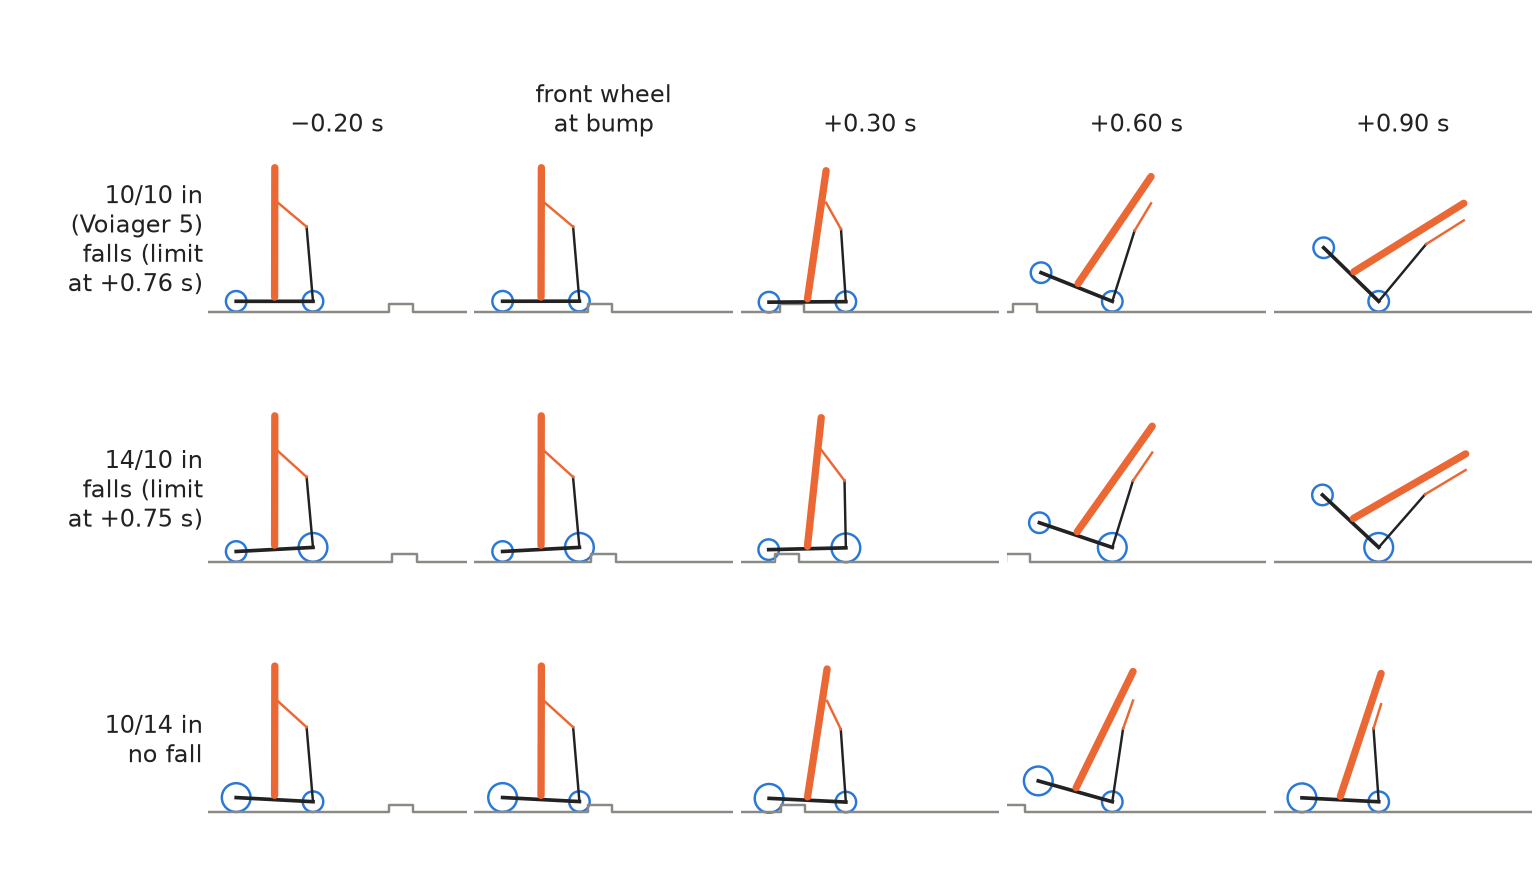
\includegraphics[width=\linewidth]{fig_d2_bump_rear_strike.png}
\caption{Key frames, short sharp-edged bump 90 mm high and 300 mm long at 15 km/h, model
with the front spring. The front wheels cross; about 0.3 s later the rigid rear wheel
strikes the edge and, with 10 in rear wheels, the scooter pitches forward. With a 14 in
rear wheel (10/14) the model does not fall. One run per configuration; an open question,
not a result about rear-wheel size (text).}\label{fig:D2}
\end{figure}

Figures~\ref{fig:Dfallsa}--\ref{fig:Dgb} give the full bump results behind Table~\ref{tab:D1}.

\FloatBarrier

\begin{figure}[htbp]
\centering
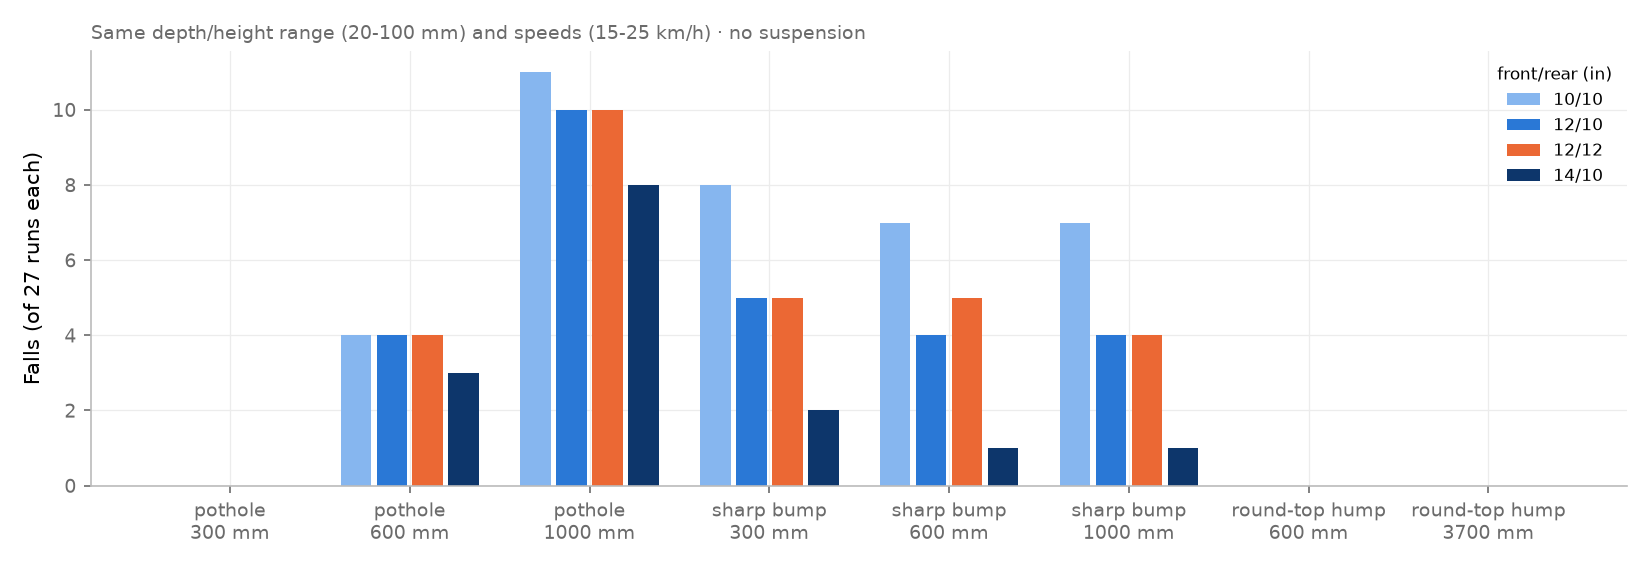
\includegraphics[width=\linewidth]{sim/bump_falls_nofork.png}
\caption{Falls by obstacle type and length, model without front suspension, per wheel configuration (same depth or height range, 20--100 mm, and speeds, 15--25 km/h). Exploratory; bump results are not validated against measurements.}\label{fig:Dfallsa}
\end{figure}

\begin{figure}[htbp]
\centering
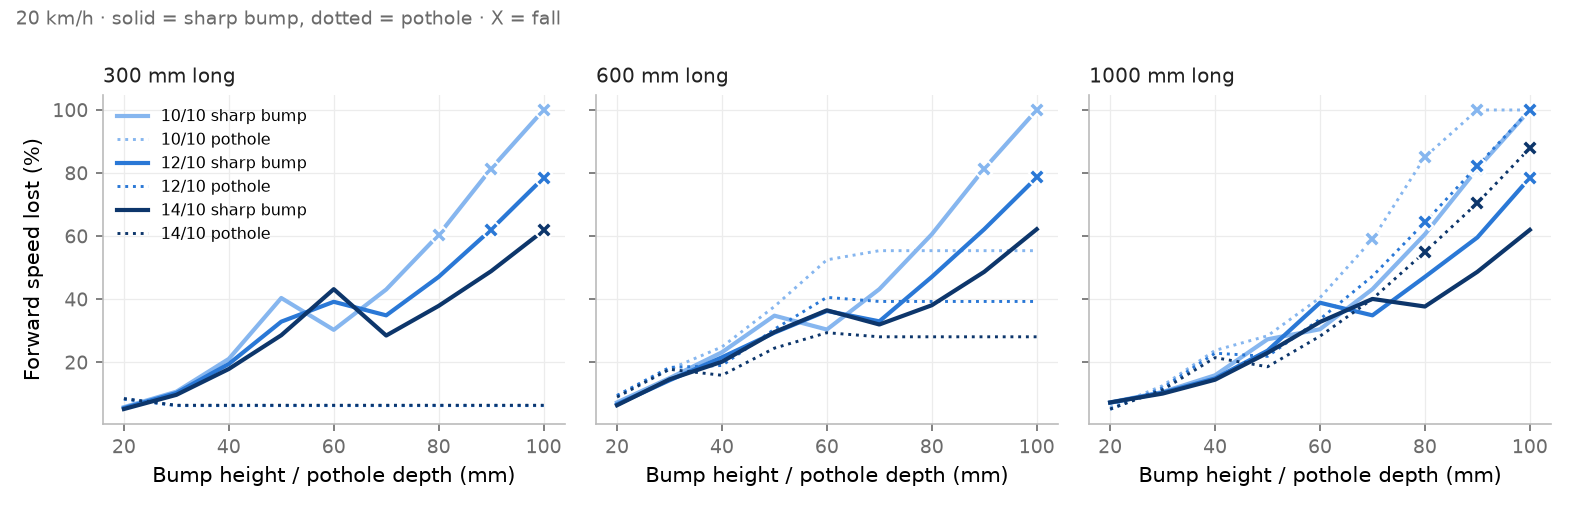
\includegraphics[width=\linewidth]{sim/bump_vs_pothole_nofork.png}
\caption{Forward speed lost on sharp-edged bumps (solid) and potholes of the same size (dotted), 20 km/h, model without front suspension; X marks a fall. Exploratory; bump results are not validated against measurements.}\label{fig:Dvsa}
\end{figure}

\begin{figure}[htbp]
\centering
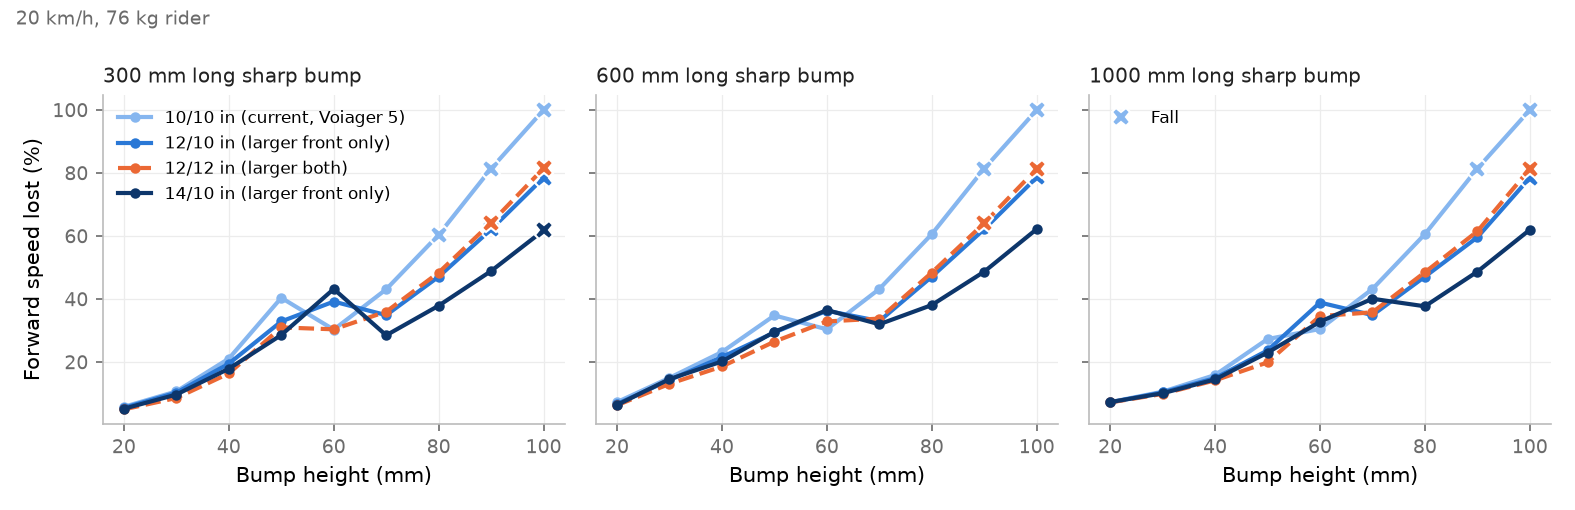
\includegraphics[width=\linewidth]{sim/bump_speedloss_nofork.png}
\caption{Forward speed lost on bumps by height, length and wheel configuration, model without front suspension. Exploratory; bump results are not validated against measurements.}\label{fig:Dspeeda}
\end{figure}

\begin{figure}[htbp]
\centering
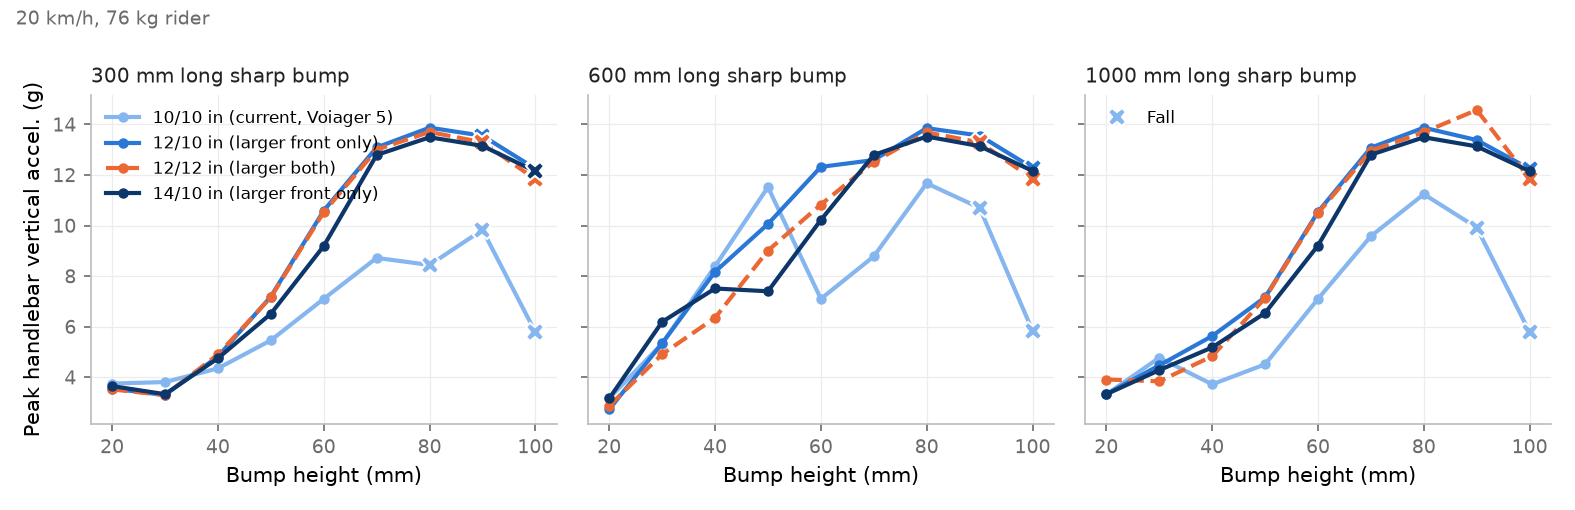
\includegraphics[width=\linewidth]{sim/bump_handlebar_nofork.png}
\caption{Simulated handlebar peak on bumps, model without front suspension. Values above the measured 1.0--2.97 g range are not supported by any measurement. Exploratory; bump results are not validated against measurements.}\label{fig:Dga}
\end{figure}

\begin{figure}[htbp]
\centering
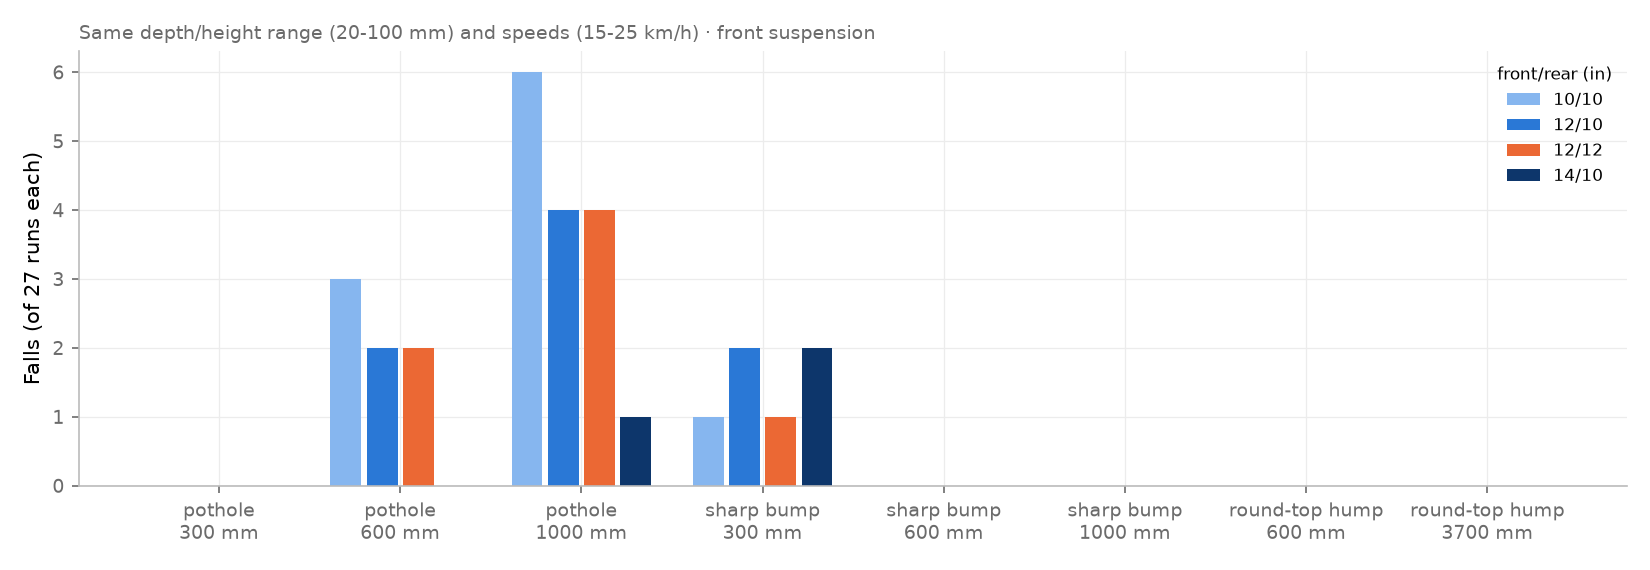
\includegraphics[width=\linewidth]{sim/bump_falls_fork.png}
\caption{Falls by obstacle type and length, model with the front spring, per wheel configuration (same depth or height range, 20--100 mm, and speeds, 15--25 km/h). Exploratory; bump results are not validated against measurements.}\label{fig:Dfallsb}
\end{figure}

\begin{figure}[htbp]
\centering
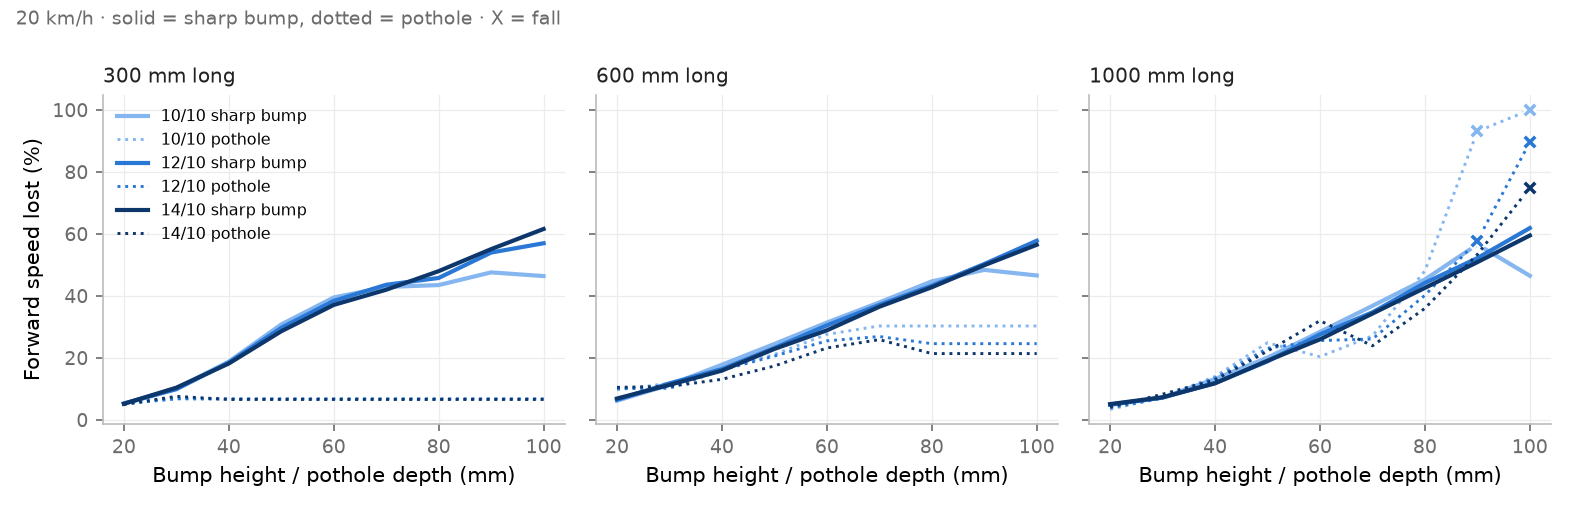
\includegraphics[width=\linewidth]{sim/bump_vs_pothole_fork.png}
\caption{Forward speed lost on sharp-edged bumps (solid) and potholes of the same size (dotted), 20 km/h, model with the front spring; X marks a fall. Exploratory; bump results are not validated against measurements.}\label{fig:Dvsb}
\end{figure}

\begin{figure}[htbp]
\centering
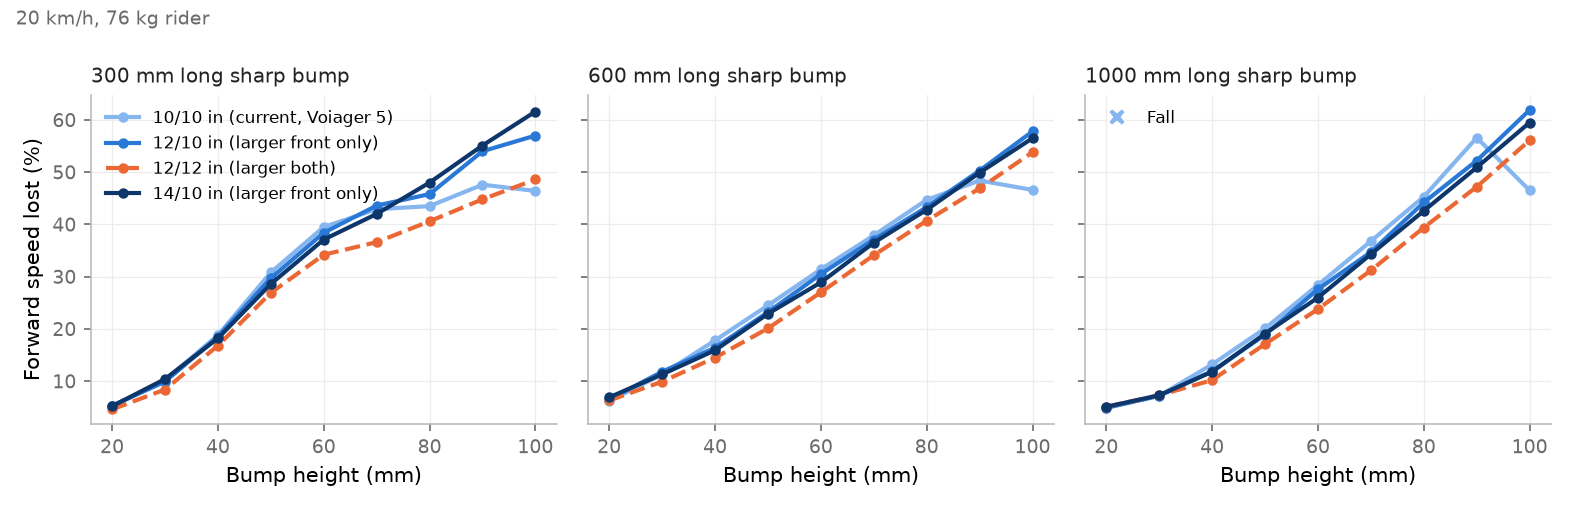
\includegraphics[width=\linewidth]{sim/bump_speedloss_fork.png}
\caption{Forward speed lost on bumps by height, length and wheel configuration, model with the front spring. Exploratory; bump results are not validated against measurements.}\label{fig:Dspeedb}
\end{figure}

\begin{figure}[htbp]
\centering
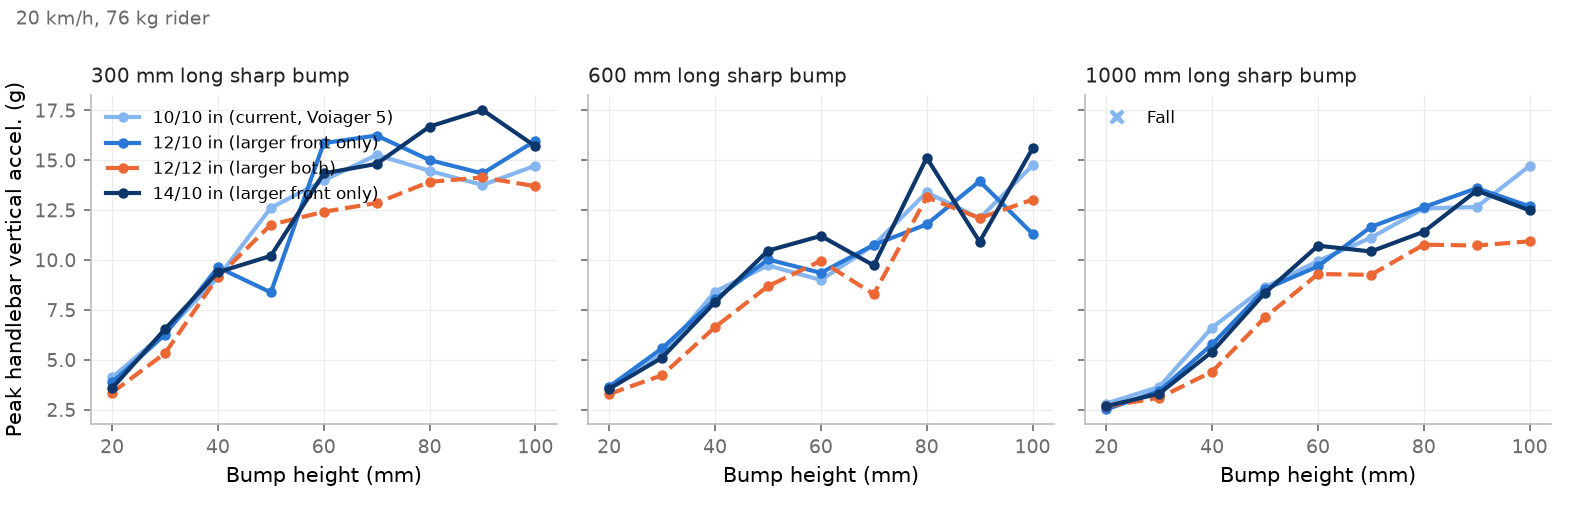
\includegraphics[width=\linewidth]{sim/bump_handlebar_fork.png}
\caption{Simulated handlebar peak on bumps, model with the front spring. Values above the measured 1.0--2.97 g range are not supported by any measurement. Exploratory; bump results are not validated against measurements.}\label{fig:Dgb}
\end{figure}

\textbf{Uncertainties and what these results cannot show.}
\begin{itemize}
\item \emph{Contact model.} On sharp bumps the two contact models agreed on the fall outcome
  in 295 of 324 runs without the fork and 307 of 324 with it (potholes: 30 of 30), with
  disagreements in both directions; the cause is not established.
\item \emph{No validation.} Modelled jolts on sharp bumps (for example 3.6--8.4 g at
  20--40 mm, 600 mm long, 20 km/h, with the fork) exceed the 1.0--2.97 g measured for 99
  of the 100 impacts in Part A, and no bumps were identified on the rides to compare with.
\item \emph{No sensitivity analysis} for bumps (tyre, rider bracing, fork parameters), and
  rear sizes were varied only on the 300 mm bump.
\item \emph{Simplifications} as for potholes: planar model, no steering, coasting, rigid rider
  pinned at the feet, idealised shapes, assumed rear wheel size.
\item \emph{Not shown:} that real bumps cause falls, that bumps are more or less dangerous than
  potholes on the road, any injury risk, or that any wheel size is safe.
\end{itemize}

\section{Further model results}\label{app:model}

These figures give the full results behind the tables and text of the model sections. All come from the same planar model or geometry model with assumed parameters (Table~\ref{tab:4}); they compare wheel configurations and are not real-world thresholds. ``With fork'' is the main model of the Voiager 5; ``no fork'' is the rigid version kept for comparison.

\subsection{Geometry model}

\begin{figure}[htbp]
\centering
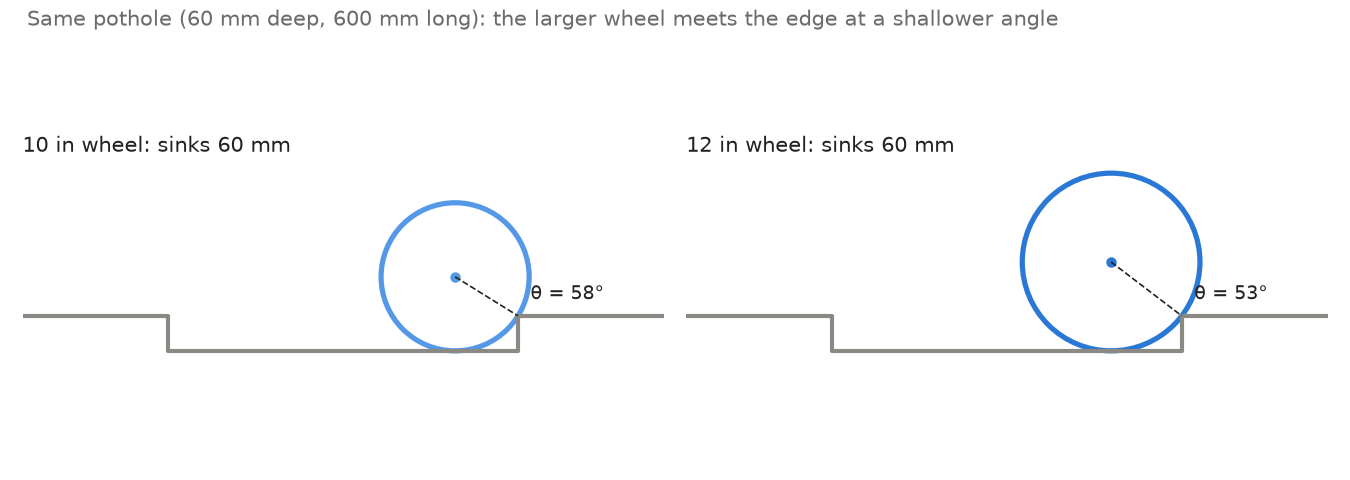
\includegraphics[width=\linewidth]{sim/geom_schematic.png}
\caption{Geometry model schematic: a 10 in and a 12 in rigid wheel at the far edge of the same 60 mm deep, 600 mm long pothole, drawn sunk to full depth for illustration. The larger wheel meets the edge at a shallower angle $\theta$.}\label{fig:E1}
\end{figure}

\begin{figure}[htbp]
\centering
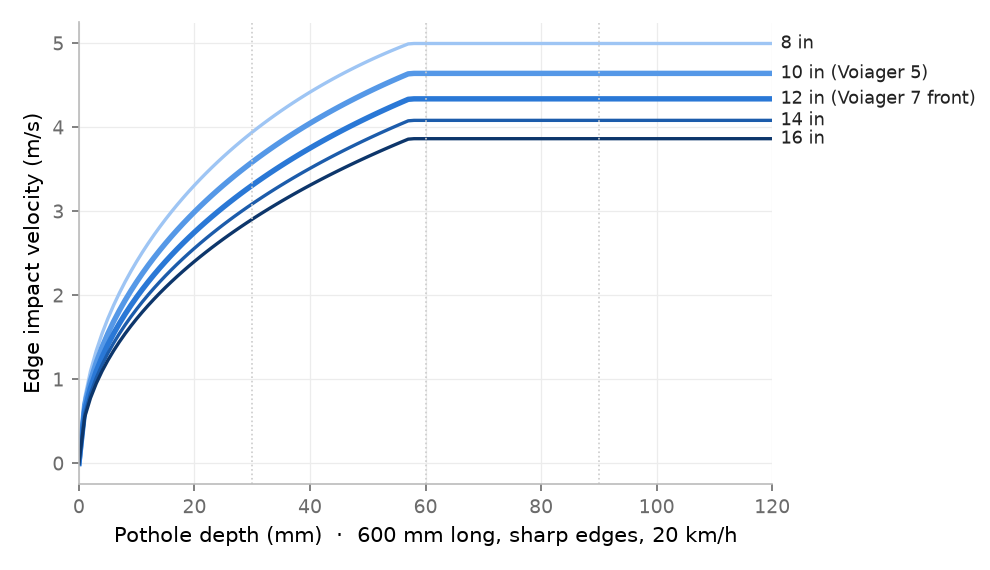
\includegraphics[width=\linewidth]{sim/geom_impact_velocity.png}
\caption{Geometry model: front-wheel edge impact velocity against pothole depth by wheel diameter (600 mm long, 20 km/h).}\label{fig:E2}
\end{figure}

\begin{figure}[htbp]
\centering
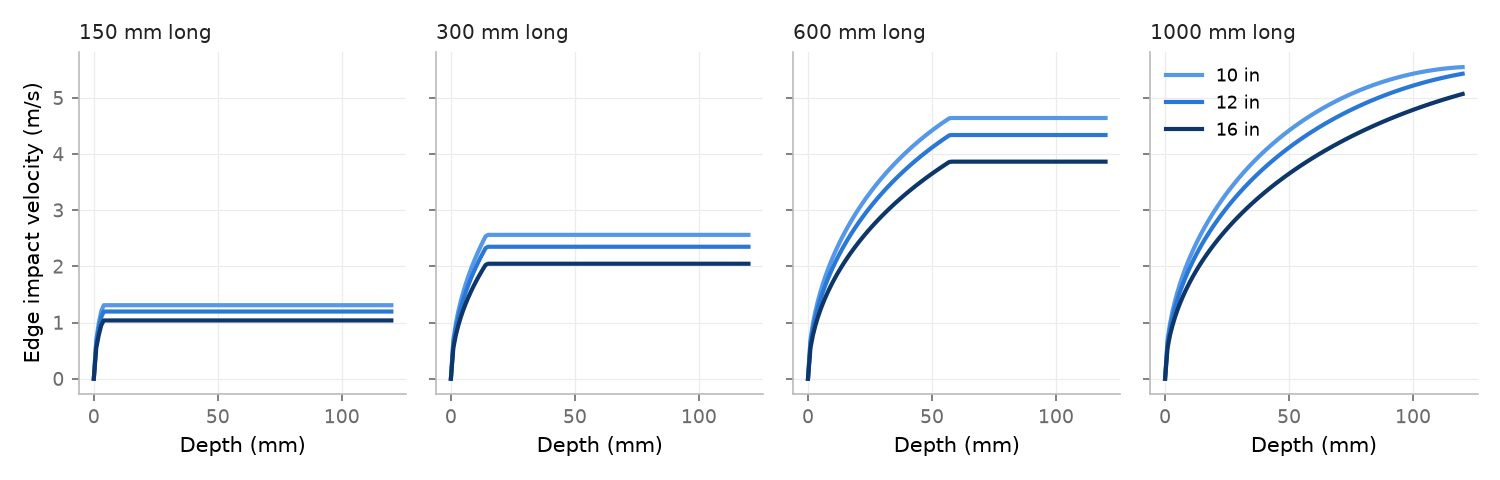
\includegraphics[width=\linewidth]{sim/geom_by_length.png}
\caption{Geometry model: edge impact velocity by pothole depth and length, 20 km/h. Short potholes limit how far the wheel can drop at speed.}\label{fig:E3}
\end{figure}

\FloatBarrier
\subsection{Main sweep}

\begin{figure}[htbp]
\centering
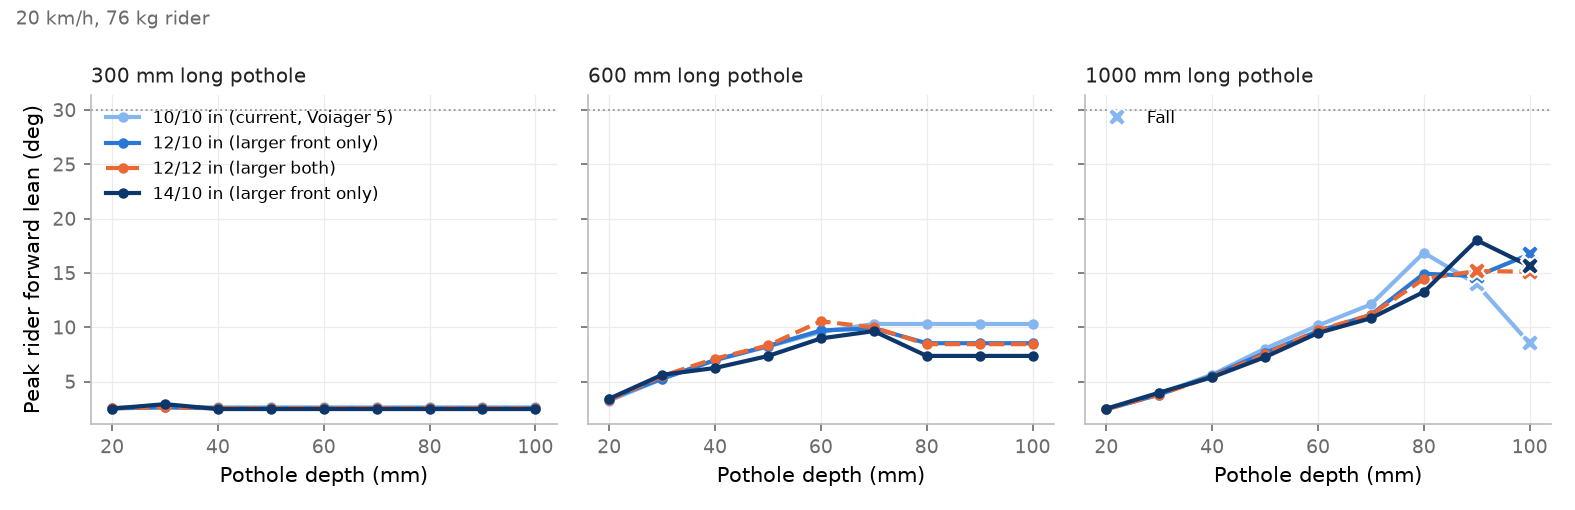
\includegraphics[width=\linewidth]{sim/sweep_lean_fork.png}
\caption{Main sweep, with front suspension (main model): peak forward lean of the rider by pothole depth and length at 20 km/h; X marks a fall. Planar model with assumed parameters (Table~\ref{tab:4}); relative comparison of wheel configurations only, not real-world thresholds.}\label{fig:Eleanfork}
\end{figure}

\begin{figure}[htbp]
\centering
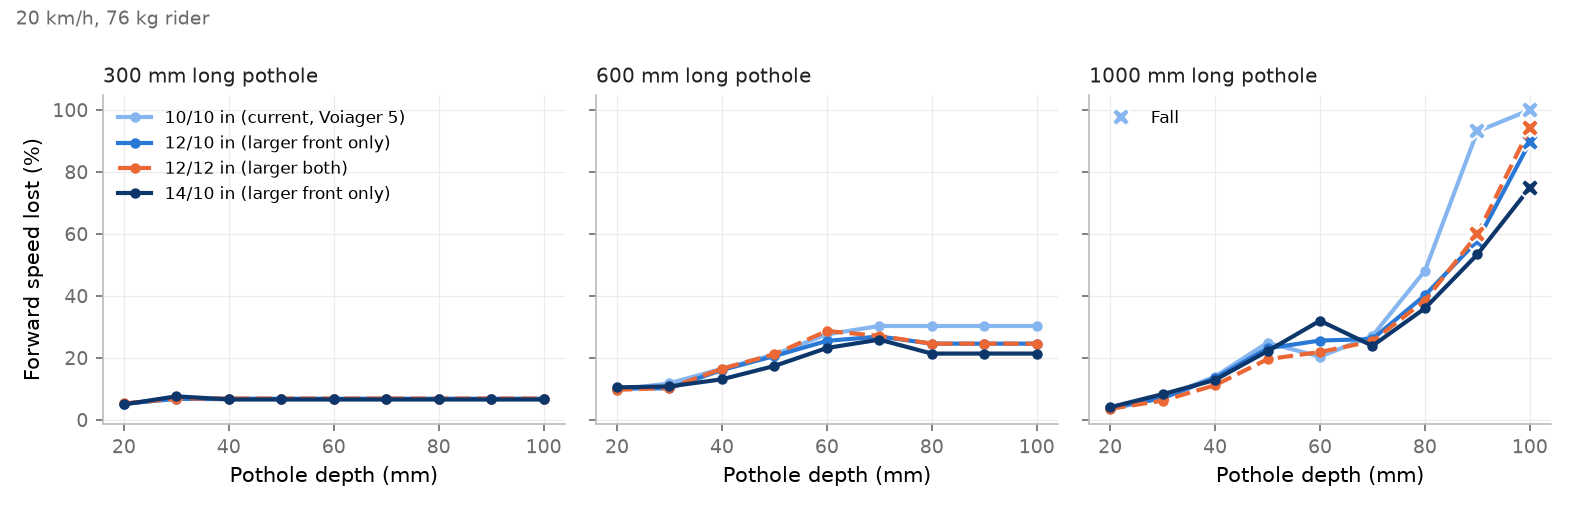
\includegraphics[width=\linewidth]{sim/sweep_speedloss_fork.png}
\caption{Main sweep, with front suspension (main model): forward speed lost crossing the pothole. Planar model with assumed parameters (Table~\ref{tab:4}); relative comparison of wheel configurations only, not real-world thresholds.}\label{fig:Espeedfork}
\end{figure}

\begin{figure}[htbp]
\centering
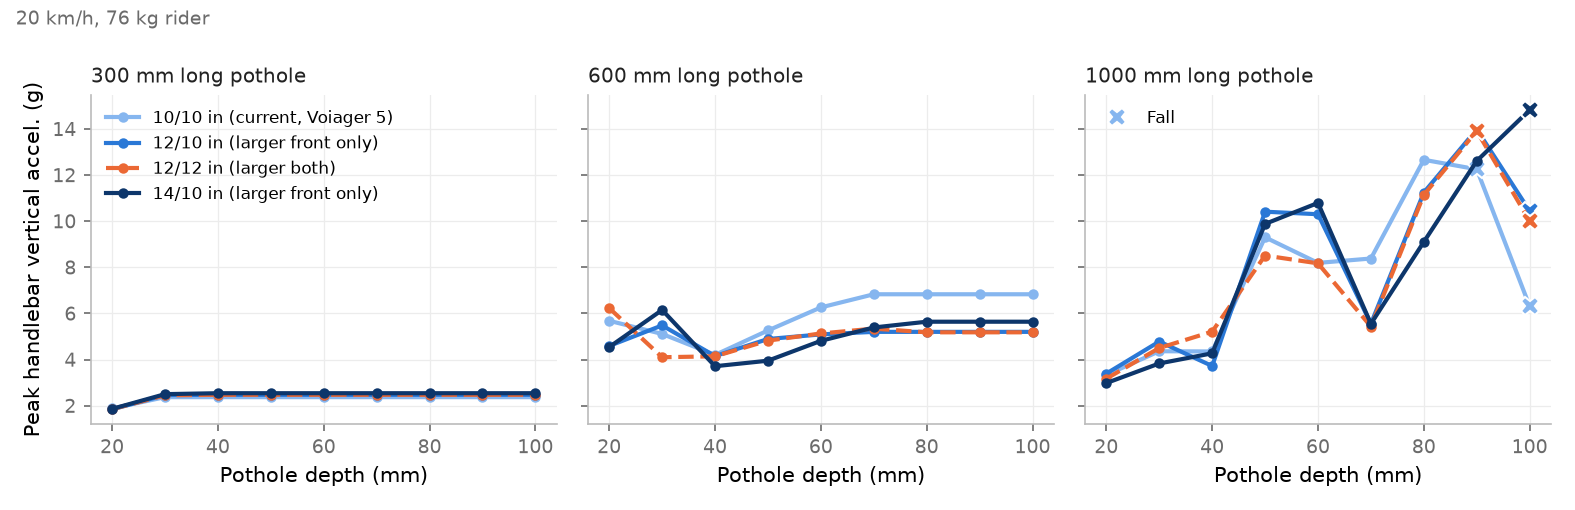
\includegraphics[width=\linewidth]{sim/sweep_handlebar_fork.png}
\caption{Main sweep, with front suspension (main model): simulated handlebar peak acceleration. Absolute values are consistent with the rides only for short potholes with the fork (Figure~\ref{fig:consistency}). Planar model with assumed parameters (Table~\ref{tab:4}); relative comparison of wheel configurations only, not real-world thresholds.}\label{fig:Egfork}
\end{figure}

\begin{figure}[htbp]
\centering
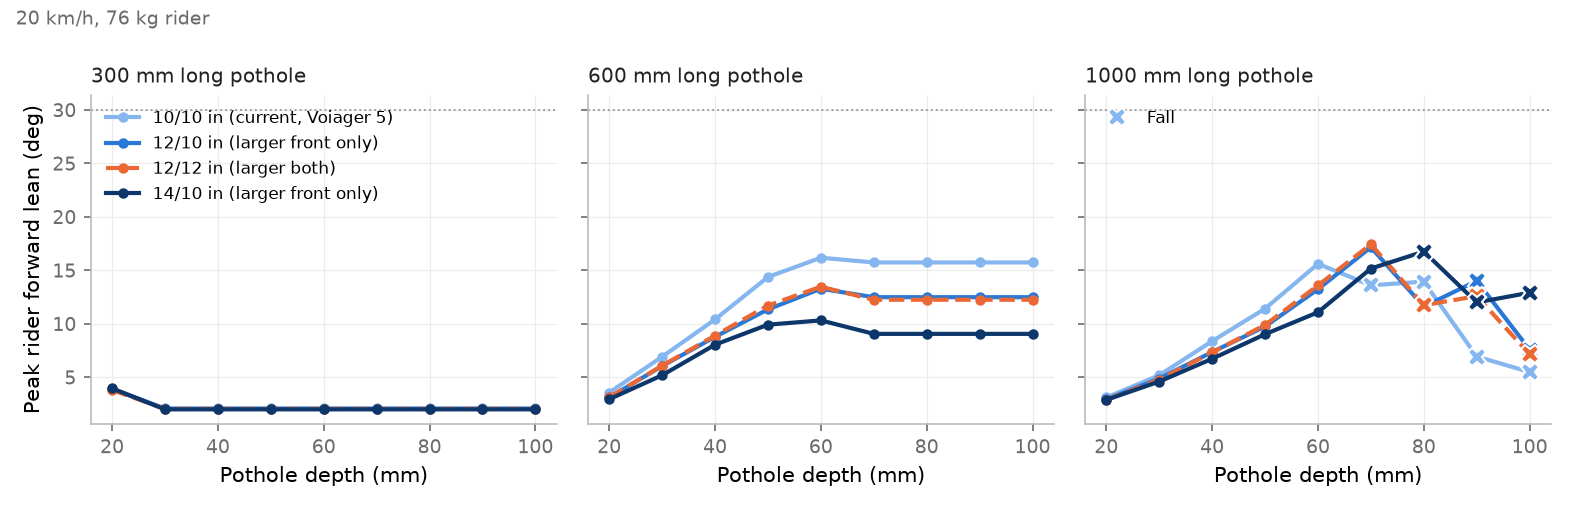
\includegraphics[width=\linewidth]{sim/sweep_lean_nofork.png}
\caption{Main sweep, without suspension: peak forward lean of the rider by pothole depth and length at 20 km/h; X marks a fall. Planar model with assumed parameters (Table~\ref{tab:4}); relative comparison of wheel configurations only, not real-world thresholds.}\label{fig:Eleannofork}
\end{figure}

\begin{figure}[htbp]
\centering
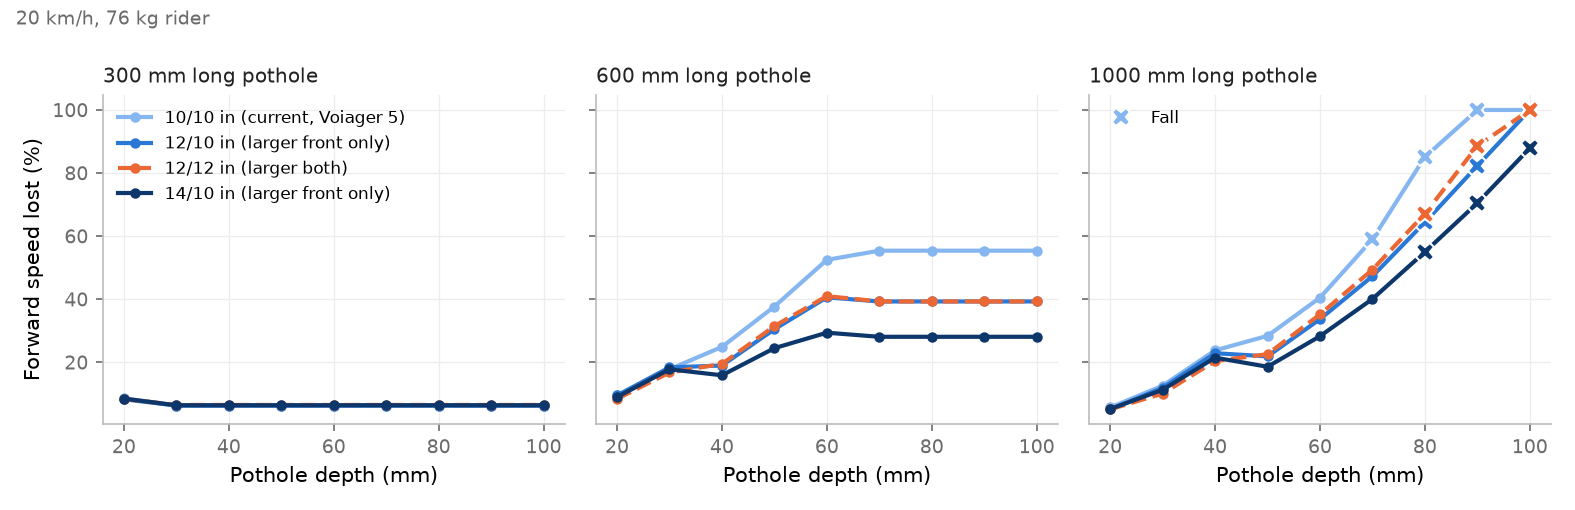
\includegraphics[width=\linewidth]{sim/sweep_speedloss_nofork.png}
\caption{Main sweep, without suspension: forward speed lost crossing the pothole. Planar model with assumed parameters (Table~\ref{tab:4}); relative comparison of wheel configurations only, not real-world thresholds.}\label{fig:Espeednofork}
\end{figure}

\begin{figure}[htbp]
\centering
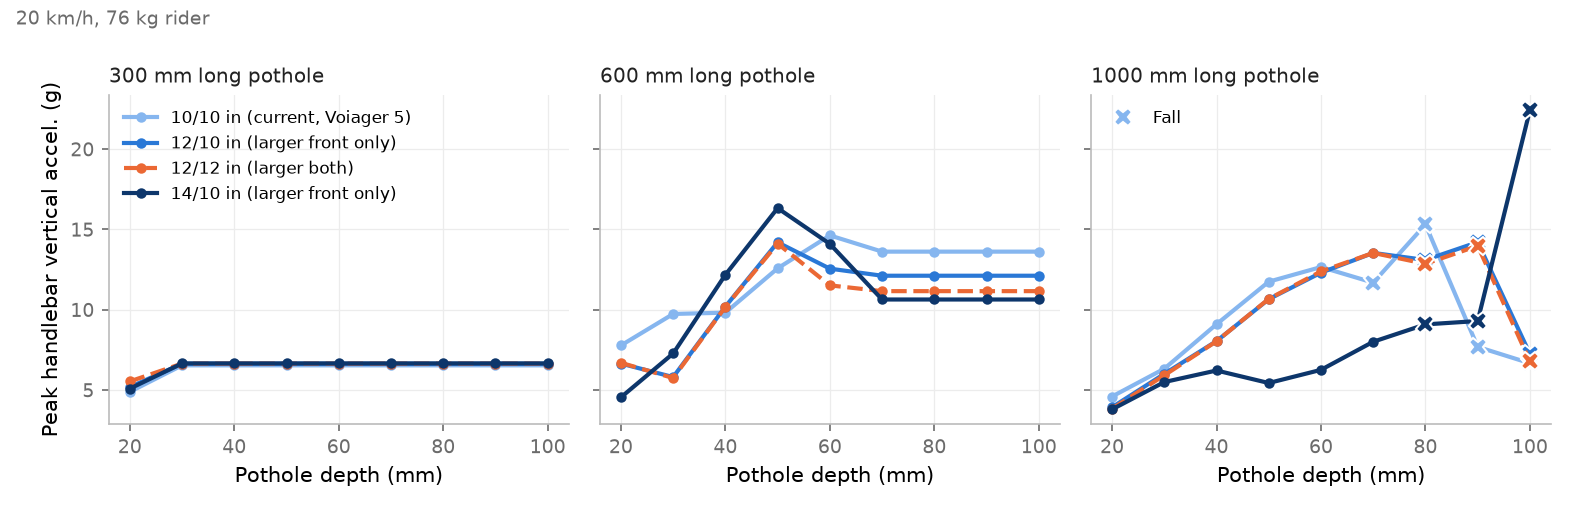
\includegraphics[width=\linewidth]{sim/sweep_handlebar_nofork.png}
\caption{Main sweep, without suspension: simulated handlebar peak acceleration. Absolute values are consistent with the rides only for short potholes with the fork (Figure~\ref{fig:consistency}). Planar model with assumed parameters (Table~\ref{tab:4}); relative comparison of wheel configurations only, not real-world thresholds.}\label{fig:Egnofork}
\end{figure}

\FloatBarrier
\subsection{Front/rear ratio study}

\begin{figure}[htbp]
\centering
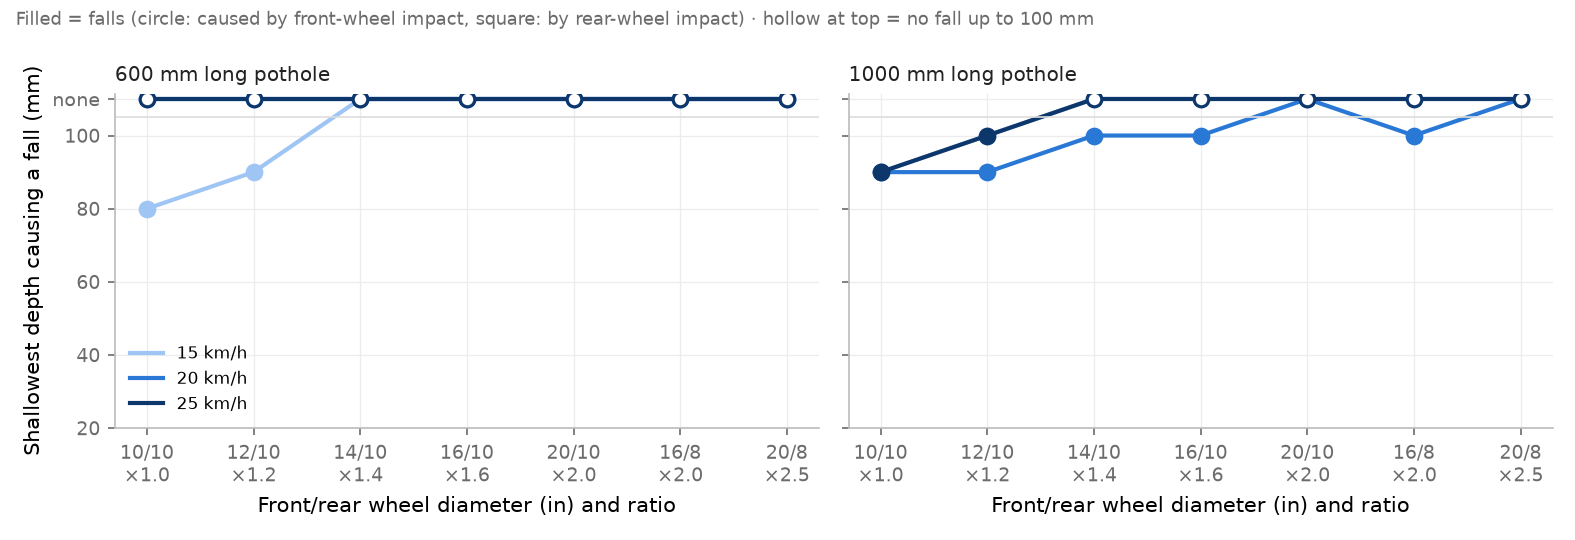
\includegraphics[width=\linewidth]{sim/ratio_first_fall_fork.png}
\caption{Ratio study, with front suspension: shallowest pothole depth (10 mm steps) at which the model fell, by front/rear diameter and speed; ``none'' = no fall up to 100 mm. No ``too large'' front wheel appeared in this planar model, which omits steering, frame geometry and cost. Planar model with assumed parameters (Table~\ref{tab:4}); relative comparison of wheel configurations only, not real-world thresholds.}\label{fig:Eratiofork}
\end{figure}

\begin{figure}[htbp]
\centering
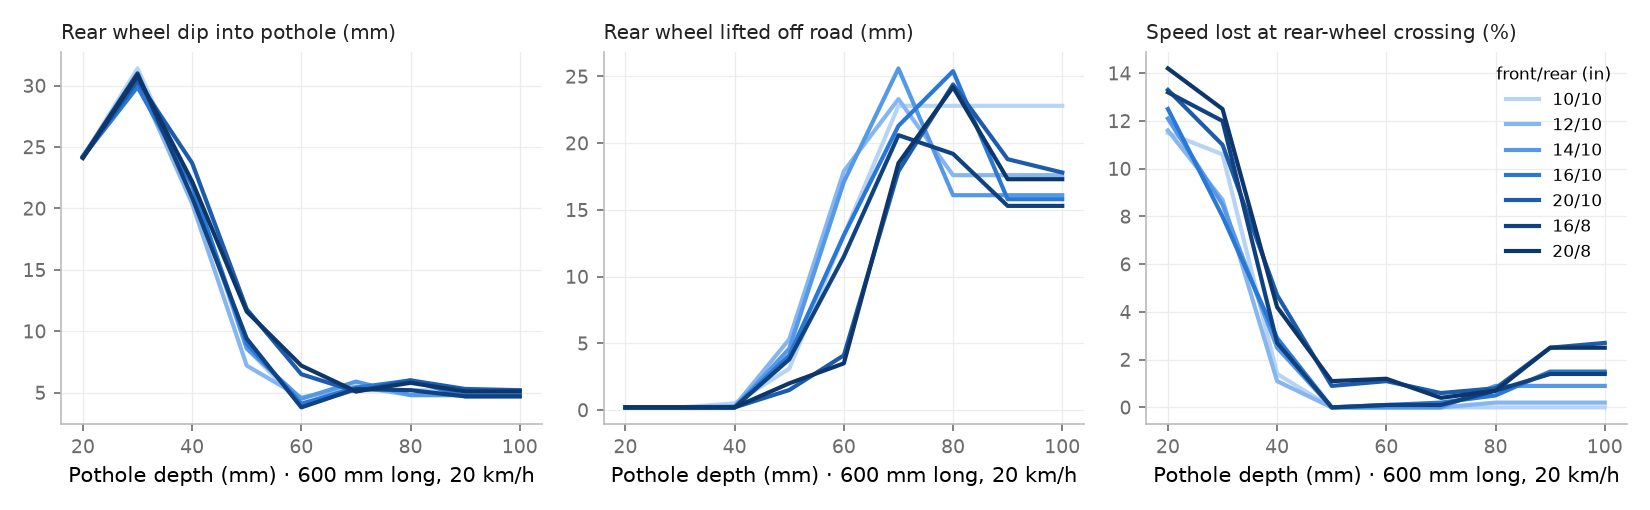
\includegraphics[width=\linewidth]{sim/ratio_rear_wheel_fork.png}
\caption{Ratio study, with front suspension: rear-wheel behaviour on a 600 mm pothole at 20 km/h (dip into the pothole, lift off the road, speed lost at the rear crossing). With the fork the configurations differ little, and the rear wheel is lifted by at most about 25 mm. Planar model with assumed parameters (Table~\ref{tab:4}); relative comparison of wheel configurations only, not real-world thresholds.}\label{fig:Erearfork}
\end{figure}

\begin{figure}[htbp]
\centering
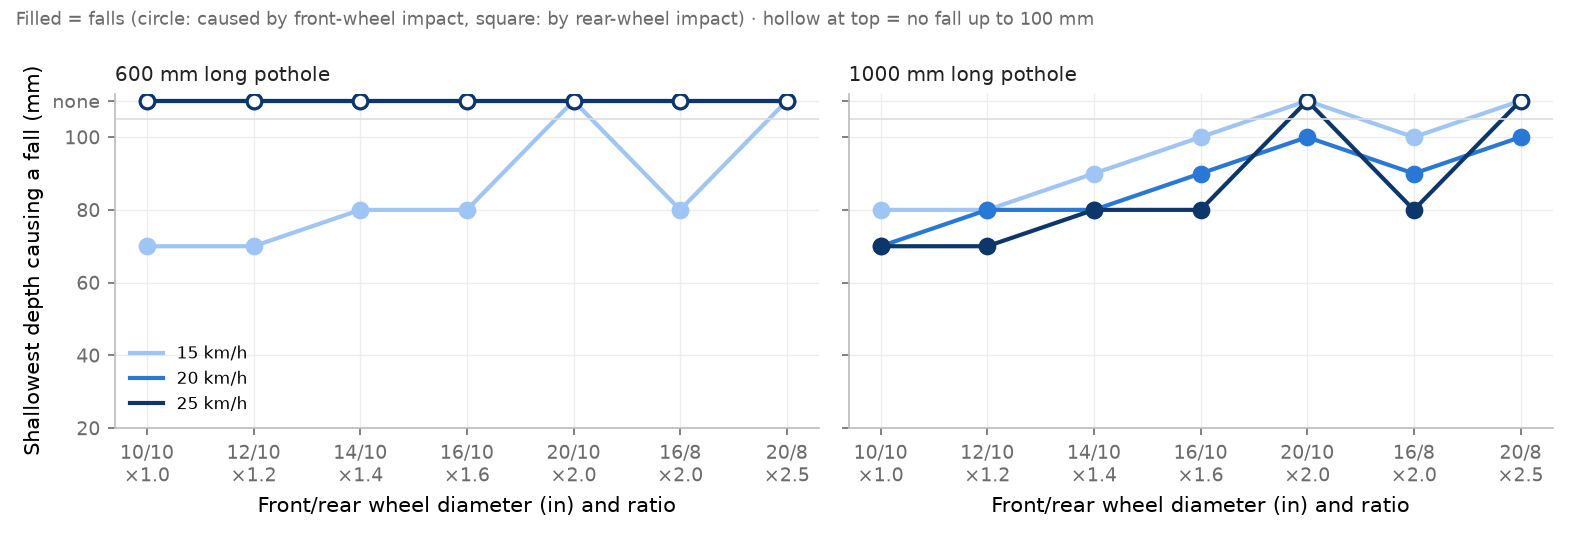
\includegraphics[width=\linewidth]{sim/ratio_first_fall_nofork.png}
\caption{Ratio study, without suspension: shallowest pothole depth (10 mm steps) at which the model fell, by front/rear diameter and speed; ``none'' = no fall up to 100 mm. No ``too large'' front wheel appeared in this planar model, which omits steering, frame geometry and cost. Planar model with assumed parameters (Table~\ref{tab:4}); relative comparison of wheel configurations only, not real-world thresholds.}\label{fig:Erationofork}
\end{figure}

\begin{figure}[htbp]
\centering
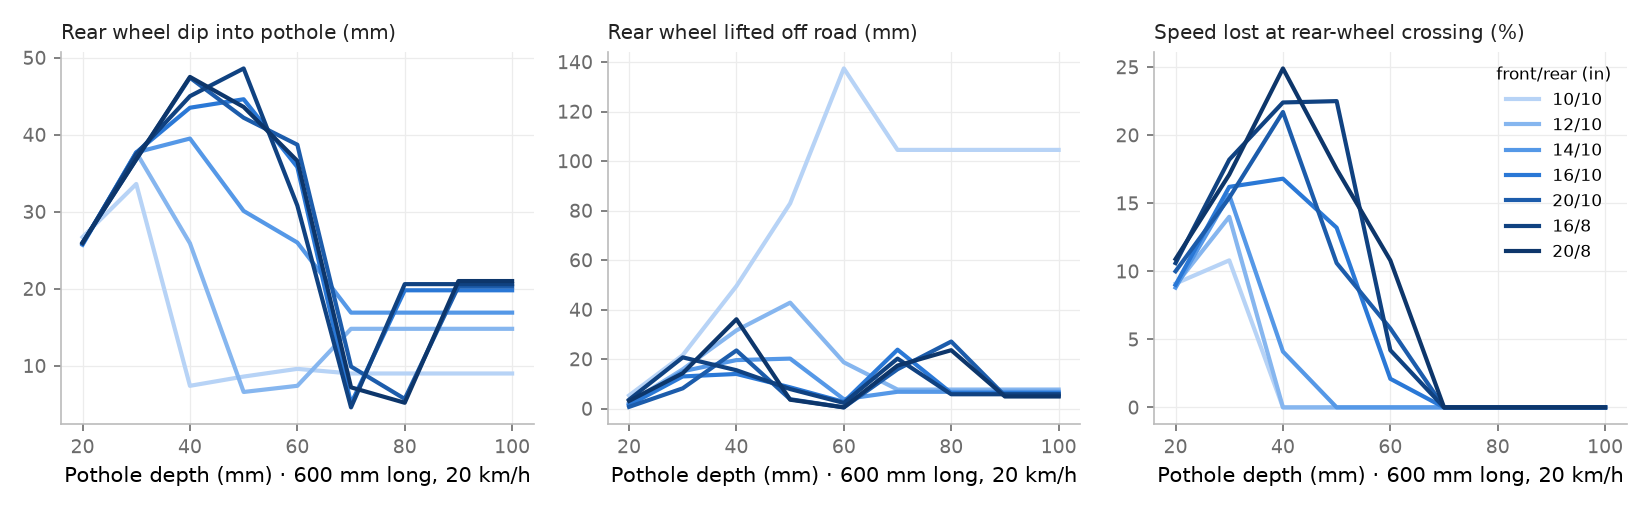
\includegraphics[width=\linewidth]{sim/ratio_rear_wheel_nofork.png}
\caption{Ratio study, without suspension: rear-wheel behaviour on a 600 mm pothole at 20 km/h (dip into the pothole, lift off the road, speed lost at the rear crossing). With small front wheels the rear is lifted clear; with large ones it drops in and gives a second jolt, which caused no falls here. Planar model with assumed parameters (Table~\ref{tab:4}); relative comparison of wheel configurations only, not real-world thresholds.}\label{fig:Erearnofork}
\end{figure}

\FloatBarrier
\subsection{Soft pothole edges}

\begin{figure}[htbp]
\centering
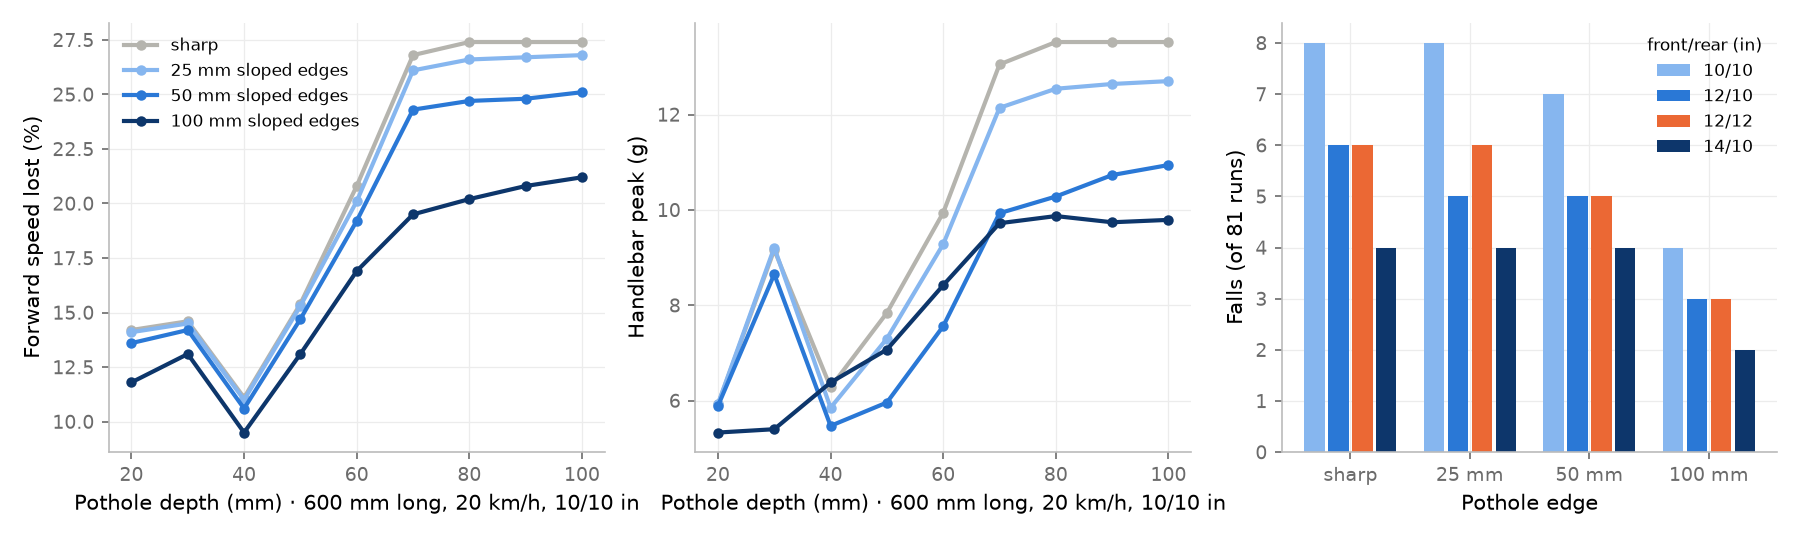
\includegraphics[width=\linewidth]{sim/soft_edges_fork.png}
\caption{Sloped (raised-cosine) pothole edges, with front suspension, profile contact model: speed lost and handlebar peak for 10/10 (600 mm, 20 km/h), and falls of 81 runs per configuration by edge width. The profile contact's absolute accelerations are too high (no tyre enveloping) and are used only for comparison between edge widths. Planar model with assumed parameters (Table~\ref{tab:4}); relative comparison of wheel configurations only, not real-world thresholds.}\label{fig:Eedges}
\end{figure}
\FloatBarrier
\subsection{Summary tables}

The tables below give the fall thresholds without suspension and the sensitivity analysis behind the statements in the model sections. Depths are on a 10 mm grid: ``80'' means a first fall between 70 and 80 mm. -- = no fall up to the deepest case simulated (100 mm). Rows in which no configuration fell are left out. All values come from the planar model with assumed parameters (Table~\ref{tab:4}) and compare configurations; they are not real-world thresholds.

% outputs/scooter_sim/fall_thresholds.csv, sim_results.csv
\begin{table}[htbp]
\centering\small
\caption{Shallowest pothole depth (mm) causing a fall, model without suspension (counterpart of Table~\ref{tab:7}). 11/10 (V5) = the Voi Voiager 5 that was ridden; 10/10 (ref.) = smaller reference wheels.}\label{tab:Enofork}
\begin{tabular}{@{}lrrrrr@{}}
\toprule
Length, speed & 10/10 (ref.) & 11/10 (V5) & 12/10 & 12/12 & 14/10 \\
\midrule
600 mm, 15 km/h & 70 & 70 & 70 & 70 & 80 \\
1000 mm, 15 km/h & 80 & 80 & 80 & 80 & 90 \\
1000 mm, 20 km/h & 70 & 70 & 80 & 80 & 80 \\
1000 mm, 25 km/h & 70 & 70 & 70 & 70 & 80 \\
\textbf{Falls (of 81 runs)} & \textbf{15} & \textbf{15} & \textbf{14} & \textbf{14} & \textbf{11} \\
\bottomrule
\end{tabular}
\end{table}

% outputs/scooter_sim/suspension/sensitivity.csv
\begin{table}[htbp]
\centering\small
\caption{Sensitivity analysis, with front suspension (main model): first fall depth (mm) on a 1000 mm pothole at 20 km/h / forward speed lost on a 60 mm deep, 600 mm pothole at 20 km/h. One parameter changed at a time from the baseline. 11/10 (V5) = the Voi Voiager 5 that was ridden; 10/10 (ref.) = smaller reference wheels.}\label{tab:Esensfork}
\begin{tabular}{@{}p{40mm}rrrrr@{}}
\toprule
Setting & 10/10 (ref.) & 11/10 (V5) & 12/10 & 12/12 & 14/10 \\
\midrule
baseline & 90 / 27.6\% & 90 / 26.8\% & 90 / 25.5\% & 90 / 28.7\% & 100 / 23.2\% \\
stiffer tyre ($\tau$ 0.015 s) & 90 / 30.2\% & 90 / 26.8\% & 90 / 25.1\% & 90 / 25.7\% & 90 / 26.3\% \\
softer tyre ($\tau$ 0.035 s) & 80 / 27.4\% & 90 / 26.7\% & 90 / 23.5\% & 90 / 23.7\% & 90 / 20.6\% \\
weaker bracing (1000 N m/rad) & 90 / 27.8\% & 90 / 29.9\% & 90 / 26.4\% & 90 / 24.7\% & 90 / 21.3\% \\
stronger bracing (3000 N m/rad) & 90 / 28.1\% & 90 / 28.3\% & 90 / 25.4\% & 90 / 25.5\% & 100 / 22.2\% \\
softer fork (15 kN/m) & 80 / 26.5\% & 80 / 24.1\% & 90 / 25.8\% & 90 / 24.6\% & 90 / 22.1\% \\
stiffer fork (40 kN/m) & 90 / 32.7\% & 90 / 25.8\% & 90 / 26.1\% & 90 / 26.9\% & 100 / 21.3\% \\
less fork damping (ratio 0.15) & 80 / 24.8\% & 80 / 24.9\% & 80 / 24.0\% & 80 / 25.4\% & 80 / 22.4\% \\
more fork damping (ratio 0.5) & 90 / 31.1\% & 90 / 29.0\% & 90 / 25.5\% & 100 / 25.4\% & 100 / 22.4\% \\
\bottomrule
\end{tabular}
\end{table}

% outputs/scooter_sim/sensitivity.csv
\begin{table}[htbp]
\centering\small
\caption{Sensitivity analysis, without suspension: first fall depth (mm) on a 1000 mm pothole at 20 km/h / forward speed lost on a 60 mm deep, 600 mm pothole at 20 km/h. One parameter changed at a time from the baseline. 11/10 (V5) = the Voi Voiager 5 that was ridden; 10/10 (ref.) = smaller reference wheels.}\label{tab:Esensnofork}
\begin{tabular}{@{}p{40mm}rrrrr@{}}
\toprule
Setting & 10/10 (ref.) & 11/10 (V5) & 12/10 & 12/12 & 14/10 \\
\midrule
baseline & 70 / 52.5\% & 70 / 47.4\% & 80 / 40.6\% & 80 / 41.0\% & 80 / 29.4\% \\
stiffer tyre ($\tau$ 0.015 s) & 60 / 69.9\% & 70 / 60.4\% & 70 / 52.4\% & 70 / 52.9\% & 80 / 36.2\% \\
softer tyre ($\tau$ 0.035 s) & 70 / 42.2\% & 80 / 38.1\% & 80 / 33.7\% & 80 / 33.4\% & 90 / 26.0\% \\
weaker bracing (1000 N m/rad) & 70 / 52.7\% & 80 / 47.9\% & 80 / 41.0\% & 80 / 42.9\% & 90 / 29.9\% \\
stronger bracing (3000 N m/rad) & 70 / 51.5\% & 70 / 45.7\% & 80 / 38.7\% & 80 / 40.0\% & 80 / 26.2\% \\
\bottomrule
\end{tabular}
\end{table}



\end{document}
